\documentclass[a5paper, 12pt]{article}

\usepackage[cm]{fullpage}
\usepackage{ulem}

\usepackage{standalone}
\usepackage{hyperref}
\hypersetup{
    colorlinks,
    citecolor=black,
    filecolor=black,
    linkcolor=black,
    urlcolor=black
}

\usepackage[utf8]{inputenc}
\usepackage[russian]{babel}

\usepackage{amssymb}
\usepackage{amsmath}
\usepackage{amscd}
\usepackage{amsthm}
\usepackage{xcolor}

\usepackage{indentfirst}

%\usepackage{marginnote} % this is used for notes on the right margin --- \marginnote{\footnotesize txt}

\usepackage{mathtools} % for mathclap command

%\usepackage[normalem]{ulem} % for crossing text out - \sout

% Redefining \def is impossible. I tried, but it is impossible.
%\let\def_prev\def

%%%%%%%%%%%%%%%%%%%%%%%%%%%%%%%%%%%%%%%%%%%%%%%
%           MATH OPERATORS SPACING            %
%%%%%%%%%%%%%%%%%%%%%%%%%%%%%%%%%%%%%%%%%%%%%%%

\let\existstemp\exists
\let\foralltemp\forall
\renewcommand{\exists}{\: \existstemp \:}
\newcommand{\existsonly}{\: \existstemp ! \:}
\renewcommand{\forall}{\: \foralltemp \:}

%%%%%%%%%%%%%%%%%%%%%%%%%%%%%%%%%%%%%%%%%%%%%%%
%            COMMAND SHORTHANDS               %
%%%%%%%%%%%%%%%%%%%%%%%%%%%%%%%%%%%%%%%%%%%%%%%

\newcommand{\example}{{\itshape Пример. }}
\newcommand{\equals}{\Leftrightarrow}
\newcommand{\exc}{{\bfseries Упражнение. }}
\newcommand{\norm}[1]{\left\| #1 \right\|}
\newcommand{\scal}[2]{\left\langle #1, #2 \right\rangle}
\newcommand{\angular}[1]{\langle #1 \rangle}

\newcommand{\Sum}[2]{\underset{#1}{\overset{#2}{\sum}}}
\newcommand{\Int}[2]{\underset{#1}{\overset{#2}{\int}}}
\newcommand{\Ker}{\text{Ker}}

% Physicists' variant of dot product
\newcommand{\pscal}[2]{\, \langle #1 | #2 \rangle \,}
\newcommand{\bra}[1]{\, \langle #1 |}
\newcommand{\ket}[1]{| #1 \rangle \,}

\renewcommand{\leq}{\leqslant}
\renewcommand{\geq}{\geqslant}

%%%%%%%%%%%%%%%%%%%%%%%%%%%%%%%%%%%%%%%%%%%%%%%
%         THEOREM DEFINITION LINES            %
%%%%%%%%%%%%%%%%%%%%%%%%%%%%%%%%%%%%%%%%%%%%%%%

\newtheorem{lem}{Лемма}[section]
\newtheorem{note}{Замечание}[section]
\newtheorem{defi}{Определение}[section]
\newtheorem{theorem}{Теорема}[section]
\newtheorem{state}{Утверждение}[section] % statement

%%%%%%%%%%%%%%%%%%%%%%%%%%%%%%%%%%%%%%%%%%%%%%%
%             GRAPHICS INCLUSION              %
%%%%%%%%%%%%%%%%%%%%%%%%%%%%%%%%%%%%%%%%%%%%%%%

\usepackage{graphicx}

\graphicspath{{./Graphics/}}

%%%%%%%%%%%%%%%%%%%%%%%%%%%%%%%%%%%%%%%%%%%%%%%
%               DRAFT TEMPLATES               %
%%%%%%%%%%%%%%%%%%%%%%%%%%%%%%%%%%%%%%%%%%%%%%%

%\usepackage{marginnotes}
\newcommand{\todo}[1]{\marginpar{\color{red} \tiny #1}}

\begin{document}
	\title{Основы функционального анализа и теории функций, четвёртый семестр.}
    \author
    {
		Лектор --- Тресков Сергей Андреевич\\
		Лекции записаны Ремневым Михаилом
    }
    \date{2013 год}
    \maketitle
    
    \tableofcontents % Вроде ок.

	\pagebreak
	
    \documentclass[12pt]{article}

\usepackage[utf8]{inputenc}
\usepackage[russian]{babel}

\usepackage{amssymb}
\usepackage{amsmath}
\usepackage{amscd}
\usepackage{amsthm}
\usepackage{xcolor}

\usepackage{indentfirst}

%\usepackage{marginnote} % this is used for notes on the right margin --- \marginnote{\footnotesize txt}

\usepackage{mathtools} % for mathclap command

%\usepackage[normalem]{ulem} % for crossing text out - \sout

% Redefining \def is impossible. I tried, but it is impossible.
%\let\def_prev\def

%%%%%%%%%%%%%%%%%%%%%%%%%%%%%%%%%%%%%%%%%%%%%%%
%           MATH OPERATORS SPACING            %
%%%%%%%%%%%%%%%%%%%%%%%%%%%%%%%%%%%%%%%%%%%%%%%

\let\existstemp\exists
\let\foralltemp\forall
\renewcommand{\exists}{\: \existstemp \:}
\newcommand{\existsonly}{\: \existstemp ! \:}
\renewcommand{\forall}{\: \foralltemp \:}

%%%%%%%%%%%%%%%%%%%%%%%%%%%%%%%%%%%%%%%%%%%%%%%
%            COMMAND SHORTHANDS               %
%%%%%%%%%%%%%%%%%%%%%%%%%%%%%%%%%%%%%%%%%%%%%%%

\newcommand{\example}{{\itshape Пример. }}
\newcommand{\equals}{\Leftrightarrow}
\newcommand{\exc}{{\bfseries Упражнение. }}
\newcommand{\norm}[1]{\left\| #1 \right\|}
\newcommand{\scal}[2]{\left\langle #1, #2 \right\rangle}
\newcommand{\angular}[1]{\langle #1 \rangle}

\newcommand{\Sum}[2]{\underset{#1}{\overset{#2}{\sum}}}
\newcommand{\Int}[2]{\underset{#1}{\overset{#2}{\int}}}
\newcommand{\Ker}{\text{Ker}}

% Physicists' variant of dot product
\newcommand{\pscal}[2]{\, \langle #1 | #2 \rangle \,}
\newcommand{\bra}[1]{\, \langle #1 |}
\newcommand{\ket}[1]{| #1 \rangle \,}

\renewcommand{\leq}{\leqslant}
\renewcommand{\geq}{\geqslant}

%%%%%%%%%%%%%%%%%%%%%%%%%%%%%%%%%%%%%%%%%%%%%%%
%         THEOREM DEFINITION LINES            %
%%%%%%%%%%%%%%%%%%%%%%%%%%%%%%%%%%%%%%%%%%%%%%%

\newtheorem{lem}{Лемма}[section]
\newtheorem{note}{Замечание}[section]
\newtheorem{defi}{Определение}[section]
\newtheorem{theorem}{Теорема}[section]
\newtheorem{state}{Утверждение}[section] % statement

%%%%%%%%%%%%%%%%%%%%%%%%%%%%%%%%%%%%%%%%%%%%%%%
%             GRAPHICS INCLUSION              %
%%%%%%%%%%%%%%%%%%%%%%%%%%%%%%%%%%%%%%%%%%%%%%%

\usepackage{graphicx}

\graphicspath{{./Graphics/}}

%%%%%%%%%%%%%%%%%%%%%%%%%%%%%%%%%%%%%%%%%%%%%%%
%               DRAFT TEMPLATES               %
%%%%%%%%%%%%%%%%%%%%%%%%%%%%%%%%%%%%%%%%%%%%%%%

%\usepackage{marginnotes}
\newcommand{\todo}[1]{\marginpar{\color{red} \tiny #1}}

\begin{document}

\section{Геометрия пространств со скалярным произведением}

	\lecture{1}

	\begin{defi} 
		\textbf{Векторное пространство} -- это математическая структура, которая формируется набором элементов, называемых векторами, для 
		которых определены операции сложения друг с другом и умножения на число -- скаляр.
	\end{defi}

	Некоторые примеры векторных пространств:
		\begin{itemize}
			\item Пространства вещественных и комплексных числе $\mathbb{R}^n$ и $\mathbb{C}^n$.
			\item Пространство непрерывных функций $C[a,b]$.
			\item Пространство интегрируемых функций $\mathbb{L}_1$, а так же $\mathbb{L}_p$ -- пространство измеримых 
			функций $f$ таких, что $p$-я их степень $|f|^p$ интегрируема.
			\item Пространства функций медленного роста ($\mathbb{S}$) и финитных ($\mathbb{D}$), а также построенные по ним пространства 
			обобщённых функций $\mathbb{S}'$ и $\mathbb{D}'$.
			\item Пространство последовательностей $l_2 : x = (x_1, x_2, ...)$ таких, что $\sum_{i=1} |x_i|^2 < \infty$, а так же 
			пространство ограниченных последовательностей $m = l_\infty : x = (x_1, x_2, ...)$
		\end{itemize}

	В данном курсе преимущественно рассматриваются векторные пространства $\mathbb{L}_2$ и $l_2$. Сразу стоит заметить, что 
	среди перечисленных пространств только $\mathbb{R}^n$ и $\mathbb{C}^n$ имеют конечную размерность, остальные -- бесконечномерны.
	
	\begin{defi}
		Произвольное множество векторов из векторного пространства E называется \textbf{линейно независимым}, если каждое конечное
		подмножество векторов, лежащее в E, тоже линейно независимо.
	\end{defi}
	
	\begin{defi}
		\textbf{Метрическим пространством} называется непустое множество $M$,
		в котором определено расстояние $\rho$ между любой парой элементов. 
	\end{defi}
	
	Обозначается -- (M, $\rho$), $\rho : M^2 \rightarrow 
	\mathbb{R}$, причём для $\rho$ выполняются следующие условия:
	\begin{enumerate}
		\item $\rho(x,y) \geq 0$~$\&$~$(\rho = 0 \equals x=y)$
		\item $\rho(x,y) = \rho(y,x)$
		\item $\rho(x,z) \leq \rho(x,y) + \rho(y,z)$ (неравенство треугольника)
	\end{enumerate}
	
	Так же, как и в курсе математического анализа, введём определение открытой элементарной окрестности:
	$$B(x, \varepsilon) = \{y \in M | \rho(x,y) < \varepsilon\}$$
	
	Таким образом, возможно определение предела как в терминах расстояний, так и в терминах окрестностей. Здесь приводится первое 
	определение, а второе остаётся в качестве упражнения:
	
	\begin{defi}
		\textbf{Пределом} функции $f : M_1 \rightarrow M_2$ называется $y~\in~M_2$, такой что 
		$$\forall \varepsilon > 0 ~\exists 
		\delta(\varepsilon) > 0, \forall x \in M_1 ~\&~ x  \neq x_0 : $$
		$$\rho_1(x, x_0) < \delta \Rightarrow \rho_2(f(x), y) < \varepsilon$$
	\end{defi}
	
	Обозначение: $lim_{x \rightarrow x_0} f(x) = y$
	
	\begin{defi}
		Назовём подмножество $U \subset M$ \textbf{открытым}, если любая точка в нём содержится вместе с некоторой окрестностью.
	\end{defi}
	
	\example Рассмотрим дискретное метрическое пространство:
	$$
		\rho = 
		\begin{cases}
			1, x \neq y \\
			0, x = y
		\end{cases}
	$$
	Любое подмножество, содержащееся в пространстве с такой метрикой является открытым: каждая точка содержит окрестность радиуса 
	$\frac{1}{2}$.
	
	\begin{defi}
		Множество M называется \textbf{замкнутым}, если оно содержит все свои предельные точки.
	\end{defi}
	
	\begin{defi}
		\textbf{Замыкание} множества -- это объединение множества и всех его предельных точек. Обозначают $\overline{M}$ или $cl ~ M$.
	\end{defi}
	
	\exc Доказать, что замыкание множества является замкнутым.
	
	\exc Доказать, что дополнение к открытому множеству замкнуто, а к замкнутому открыто.
	
	\begin{defi}
		$M_1 \subset M$, $M_2 \subset M$. Подмножество $M_1$ \textbf{плотно} в $M_2 \equals M_2 \subset \overline{M}_1$
	\end{defi}
	
	\example Множество рациональных чисел плотно в множестве иррациональных.
	
	\begin{defi}
		Пусть $M_1 \subset M$. $M_1$ \textbf{всюду плотно} $\equals$ $\
		\overline{M}_1 = M$. (То есть для любой точки из M существует 
		последовательность из $M_1$, которая сходится к этой точке.)
	\end{defi}
	
	\begin{defi}
		Множество M называется \textbf{сепарабельным}, если у него найдётся счётное, всюду плотное подмножество.
	\end{defi}
	
	\begin{defi}
		\textbf{Счётное множество} -- множество, все элементы которого можно пронумеровать.
	\end{defi}

	{\color{gray} Немного о счётности. Самым простым примером счётного множества является множество натуральных чисел $\mathbb{N}$, поскольку нумерация элементов множества как раз и производится натуральными числами. Множество рациональных чисел $\mathbb{Q}$ так же счётно (поскольку его можно представить в виде прямого произведения $\mathbb{N}$ на само себя, а произведение счётных множеств -- счётно), множества $\mathbb{R}$ и $\mathbb{C}$ несчётны.}
	
	\begin{defi}
		Последовательность $\{x_n\}$ называется \textbf{фундаментальной} (или \textbf{последовательностью Коши}), если она 
		удовлетворяет \textbf{условию Коши}:
		$$\forall \varepsilon > 0 ~\exists N = N(\varepsilon),~ \forall n_1, n_2 > N,~ \rho(x_{n_1}, x_{n_2}) < \varepsilon$$
	\end{defi}

	\begin{defi}
		Метрическое пространство называется \textbf{полным}, если любая содержащаяся в нем фундаментальная последовательность имеет 
		предел.
	\end{defi}
	
	\begin{defi}
		Назовём \textbf{нормой вектора} $x$ отображение $\|.\| : x \rightarrow \mathbb{R_+}$, для которого выполнены следующие условия:
		\begin{enumerate}
			\item $\|x\| \geq 0 ~(\|x\| = 0 \equals x = 0)$
			\item $\|\alpha x\| = |\alpha| \|x\|$
			\item $\|x + y\| \leq \|x\| + \|y\|$
		\end{enumerate}
	\end{defi}
	
	\example $\|.\|_{L_1} = \int {|f|}$, $\|.\|_{L_2} ~=~ \sqrt{\int {|f|^2}}$,  $\|.\|_{m} ~= \sup {|m_i|}$
	
	Для нормированного пространства можно легко определить метрику, вводя $\rho(x,y) = \|x-y\|$. При этом будут выполняться все аксиомы,
	определённые для метрики ранее.
	
	Можно рассмотреть два идентичных определения эквивалентности норм:
	
	\begin{defi}
		Две нормы называются \textbf{эквивалентными}, если они порождают один и тот же запас открытых множеств.
	\end{defi}
	
	\begin{defi}
		Две нормы $\rho_1$ и $\rho_2$ на пространстве V называются \textbf{эквивалентными}, если существуют две положительные константы 
		$C_1$ и $C_2$, такие, что для любого $x \in V$ выполняется 
		$$C_1 \rho_1(x) \leq \rho_2(x) \leq C_2 \rho_1(x)$$
	\end{defi}
	Эквивалентные нормы задают на пространстве одинаковую топологию. В конечномерном пространстве все нормы эквивалентны.
	
	\begin{defi}
		\textbf{Банахово пространство} -- полное нормированное пространство.
	\end{defi}
	
	\subsection{Скалярное произведение}

	Значительное внимание в курсе уделено пространствами со скалярным произведением.

	\begin{defi}
		Cкалярное произведение -- это отображение $\scal{.}{.} : E^2 \rightarrow C$, удовлетворяющее следующим свойствам:
		\begin{enumerate} 
			\item $\scal{x}{y} = \overline{\scal{y}{x}}$
			\item $\scal{\alpha x_1 + \beta x_2}{y} ~= ~\alpha \scal{x_1}{y} + \beta \scal{x_2}{y}$
			\item $\scal{x}{x} ~\geq ~0 ~(\scal{x}{x} = 0 \equals x = 0)$
		\end{enumerate}
	\end{defi}

	\begin{defi}
		$\|x\| = \sqrt{\scal{x}{x}}$ {\color{gray} Пока это <<контрабандное>> утверждение, докажем его позже.}
	\end{defi}
	
	\exc Доказать тождество параллелограмма: 
	$$\norm{x+y}^2 + \norm{x-y}^2 = 2 \norm{x}^2 + 2 \norm{y}^2$$
	Докажем неравенство Шварца (оно же неравенство Коши-Буняковского):
	\opt{В курсе линейной алгебры подобное неравенство уже доказывалось, но то доказательство было для конечномерного случая.}
	$$|\scal{x}{y}| \leq \norm{x} \cdot \norm{y}$$
	Пусть $\scal{x}{y} \neq 0$, положим 
	$$\theta = \frac{\scal{x}{y}}{|\scal{x}{y}|},\qquad t \in \mathbb{R}$$
	
	\begin{align*}
	0 \leq \norm{
	{\theta} x + t y}^2 ~&=~ \scal{\bar{\theta} x + t y}{\bar{\theta} x + t y} ~= \\
	\bar{\theta} \scal{x}{\bar{\theta} x + t y} ~&+~ t \scal{y}{\bar{\theta} x + t y} ~= \\
	|\theta|^2 \norm{x}^2 ~+~ t \bar{\theta} \scal{x}{y} ~&+~ t \theta \scal{y}{x} ~+~ t^2 \norm{y}^2 ~= \\
	t^2 \norm{y}^2 + 2t &\mod{\scal{x}{y}} + \norm{x}^2
	\end{align*}
	Дискриминант должен быть не положительным. Таким образом, получаем:
	$$|\scal{x}{y}|^2 \leq \|x\|^2 \|y\|^2$$
	Взяв квадратный корень от обеих частей выражения, получим искомое неравенство.
	
	\begin{defi}
		\textbf{Гильбертовым пространством} называется пространство со скалярным произведением, которое полно относительно нормы, 
		порождённой \off{этим} скалярным произведением.
	\end{defi}
	
	\example $\mathbb{R}^n$ -- гильбертово пространство.
	
	\begin{defi}
		$x \in l_2$, $\norm{x} = (\sum{|x_i|^2})^{1/2}$ 
	\end{defi}

	\lecture{2}

        Пора доказать <<контрабанду>>, введённую в прошлом разделе. Докажем, что норма, введённая на основе скалярного произведения, 
    $$\norm{x} = \sqrt{\scal{x}{x}}$$
    соответствует всем ранее указанным аксиомам.

    \begin{enumerate}
    \item Очевидно из первого свойства скалярного произведения.
    \item $\norm{\lambda x}^2 = \lambda \bar{\lambda} \scal{x}{x} = | \lambda |^2 \cdot \norm{x}^2$
    \item $\norm{x+y} \overset{?}{\leq} \norm{x} + \norm{y}$
	      $$\norm{x + y}^2 = \norm{x}^2 + \scal{x}{y} + \scal{y}{x} + \norm{y}^2 \leq \norm{x}^2 + 2 \norm{x} \norm{y} + \norm{y}^2
			= (\norm{x} + \norm{y})^2
	      $$
    \end{enumerate}
	Таким образом, пространство со скалярным произведением является нормированным пространством и определяет норму на нем.
	
	\begin{defi}
		Подмножество векторного пространства называется \textbf{выпуклым}, если оно содержит вместе с любыми двумя 
		точками соединяющий их отрезок.
	\end{defi}

	В доказательстве последующей теоремы потребуется данное утверждение:
	% Что-то было написано в исправлении, а что --- не разобрал.
	\begin{state}
		Скалярное произведение непрерывно по первому и второму аргументам.
		$$\scal{x}{y} - \scal{x'}{y'} = \scal{x}{y} - \scal{x'}{y} + \scal{x'}{y} - \scal{x'}{y'} \leq$$
		$$\leq \norm{x - x'}\cdot \norm{y} + \norm{x'} \cdot \norm{y - y'}$$
	\end{state}
	
	\begin{theorem}
		Пусть $G$ --- замкнутое выпуклое подмножество гильбертового пространства $H$. Тогда
		$$\forall h \in H \quad \existsonly g \in G \quad \norm{h-g} = \underset{g' \in G}{\inf} \norm{h-g'} = \alpha$$
	\end{theorem}
	\begin{proof}
		Рассмотрим последовательность $g_1, g_2, ..., g_n$ $\norm{h - g_n}~\rightarrow~\alpha$
		$$\forall \varepsilon \exists N(\varepsilon), n > N(\varepsilon) \norm{h - g_n} < \alpha + \varepsilon$$
		Примем $n, m > N(\varepsilon)$. Рассмотрим вектора $h - g_n$, $h - g_m$, запишем для них тождество параллелограмма.
		% Не понимаю, что это за выражение и зачем оно было нужно.
		% $$\norm{g_n - g_m} = 2 \cdot \norm{h - g_n} + 2 \cdot \norm{h - g_m}$$
		$$\norm{g_n - g_m}^2 = 2 \cdot \norm{h - g_n}^2 + 2 \cdot \norm{h - g_m}^2 - \norm{2h - (g_n + g_m)}^2$$
		$$\norm{g_n - g_m}^2 = 2 \cdot \norm{h - g_n}^2 + 2 \cdot \norm{h - g_m}^2 - 4 \cdot \norm{h - \frac{g_n + g_m}{2}}^2 \leq$$
		В силу выпуклости подмножества, $\frac{g_n + g_m}{2} \in G$, что означает $\norm{h - \frac{g_n + g_m}{2}} \geq \alpha$, так
		как $\alpha$ - точная нижняя грань.
		$$\leq 2 (\alpha + \varepsilon)^2 + 2 (\alpha + \varepsilon)^2 - 4 \alpha^2 = 8 \alpha \varepsilon + 4 \varepsilon^2$$
		Из этого выражения получаем, что последовательность $\norm{h - g_n}$ --- фундаментальная, следовательно найдётся $g_0$, такое,
		что $\norm{h - g_0} = \alpha$.
		
		Также докажем единственность. Пусть таких векторов найдётся два: $g'$ и $g''$. Тогда
		$$\norm{h - g'} - \norm{h - g''} = \alpha$$
		$$\norm{g' - g''}^2 = 2 \norm{h - g'}^2 + 2 \norm{h - g''}^2 - 4 \norm{h - \frac{g' + g''}{2}} \leq$$
		$$\leq 4 \alpha^2 - 4 \alpha^2 = 0$$
		$\Rightarrow g' = g'' \Rightarrow$ такой вектор найдётся только один.
	\end{proof}
	
	\begin{theorem}
		$G$ - замкнутое подпространство $H$. $h \in H, g \in G$, $g$ --- ближайший. Тогда $f = (h - g) \perp G$
	\end{theorem}
	Мы можем выделить ближайший вектор, так как подпространство обязательно является выпуклым. {\color{gray} Деваться больше некуда.}
	\begin{proof}
		Предположим, что это не так:
		$$\scal{f}{g_1} = \alpha \neq 0$$
		Рассмотрим вектор:
		$$g^* = g + \frac{\scal{f}{g_1}}{\norm{g1}^2} \cdot g_1 = $$
		$$ = g + \frac{\alpha}{\norm{g_1}^2} \cdot g_1$$
		Используя этот вспомогательный вектор, докажем ортогональность:
		$$\norm{h - g^*}^2 = \scal{h - g - \frac{\alpha}{\norm{g_1}^2} \cdot g_1}{\underset{То же самое}{...}} = $$
		$$ = \norm{h - g}^2 - \scal{h - g}{\frac{\alpha}{\norm{g_1}^2} g_1} - \scal{\frac{\alpha}{\norm{g_1}^2} g_1}{h - g} + 
		\frac{|\alpha|^2}{\norm{g_1}^2} g_1 = $$
		$$ = \norm{h - g}^2 - \frac{|\alpha|^2}{\norm{g_1}^2} - \frac{|\alpha|^2}{\norm{g_1}^2} + \frac{|\alpha|^2}{\norm{g_1}^2} = $$
		$$ = \norm{h - g}^2 - \frac{|\alpha|^2}{\norm{g_1}^2}$$
		То есть получается, что $g^*$ ближе к $h$, чем $g$, что противоречит условию теоремы. Следовательно $\alpha = 0$.
	\end{proof}
	
	Таким образом, любой вектор гильбертова пространства единственным
	способом представляется в виде суммы двух векторов:
	$g \in G$ ($G$ --- замкнутое подпространство $H$) и $g_2 \in G^\perp$ ($G^\perp$ --- ортогональное дополнение к $G$).
	А это значит, что $H = H_1 \oplus H_1^\perp$
	
	Пусть существует ортонормированная последовательность $e_1, e_2, ..., e_n, ...$. Рассмотрим линейную 
	оболочку первых $n$ элементов $E_n = \{ \sum_1^n \alpha_i e_i \}$.

	Для $h \in H$ найдётся такое $g_n \in E_n$, что $f_n = h - g_n \perp E_n$, причём 
	$g_n = \sum_1^n \alpha_i e_i$. Коэффициенты $\alpha_i$ находятся из условия ортогональности $f_n$ и $E_n$:

    $$
        \left.
        \begin{aligned}
            \scal{f_n}{e_i} = \scal{h}{e_i} - \scal{g_n}{e_i} \\
            \scal{f_n}{e_i} = 0
        \end{aligned}
        \right\} \Rightarrow \alpha_i = \scal{g_n}{e_i} = \scal{h}{e_i}
    $$

	Для $h = g + f$, (так как $\scal{g}{f} = 0$)
	$$ \norm{h}^2 = \norm{g_n}^2 + \norm{f_n}^2 = \sum_1^n |\alpha_i|^2 + \norm{f_n}^2$$
	Имеет смысл рассмотреть такую величину в гильбертовом пространстве: 
	$h = \sum_1^{\infty} \alpha_i e_i,\, \alpha_i = \scal{h}{e_i}$ -
	\textbf{ряд Фурье} вектора h.
	$$ \norm{h}^2 \geq \sum_1^n |\alpha_i|^2 = \norm{g_n}^2 $$

	%%	Точно ли в выражении выше стоит \geq? Это стоит проверить.
	
	Таким образом, мы вывели \textbf{неравенство Бесселя}:
	$$ \norm{h}^2 \geq \sum_{i=1}^{\infty} \mod{\alpha_i}^2 $$

	Это неравенство гарантирует сходимость ряда $\sum_1^{\infty} |\alpha_i|^2$, что обеспечивает фундаментальность 
	последовательности векторов $g_n$.
	
	\begin{defi}
		Ортонормированную систему будем называть \textbf{полной}, если её нальзя пополнить 
		(то есть добавить единичный вектор $e_{n+1}$, перпендикулярный предыдущим).
	\end{defi}
	\begin{defi}
		Ортонормированную систему будем называть \textbf{замкнутой}, если для любого вектора из 
		гильбертова пространства неравенство Бесселя становится равенством.
	\end{defi}
	
	\begin{state}
		Пусть система векторов $\{ e_\alpha \}$ полна, тогда $\overline{ \nu \{ e_\alpha \} } = H$.
	\end{state}
	\begin{proof}
		Предположим, что это не так. Пусть $h_0 \notin \overline{ \nu \{ e_\alpha \} }$, тогда найдётся ближайший вектор $\Rightarrow 
		\exists f_0 	= (h_0 - g_0)^\perp	\Rightarrow$ систему $\{ e_{\alpha} \}$ можно пополнить.
	\end{proof}
	
	%{\huge НЯ!}

	\lecture{3}

	Перейдём к основному содержанию нашего курса --- гильбертовым пространствам. Пространствами, рассматриваемыми 
	в дальнейших лекциях будут:
	\begin{itemize}
		\item $\mathbb{L}_2(\mathbb{X})$ \\
		$\scal{f}{g} \overset{df}{=} \int_{\mathbb{X}} f\overline{g}$ \\
		$\norm{f}_2 = \sqrt{\int_{\mathbb{X}} |f|^2}$ \\
		% Вот я нехороший человек, такого упражнения же не задавали :)
		%\exc Доказать полноту $\mathbb{L}_2$.
		
		\item $l_2$ \\
		В первой и второй лекциях свойства этого пространства уже были подробным образом рассмотрены. \\
		\exc Доказать полноту $l_2$.
	\end{itemize}
	Пространства $l_2$ и $\mathbb{L}_2$ ---полные, сепарабельные и бесконечномерные пространства.
	
	В прошлой лекции было рассмотрено неравенство Бесселя: \\
	$$\norm{h}^2 \geq \sum_{k=1}^{\infty}\scal{h}{e_k}$$
	Где $h = \sum_{n=1}^{\infty} \alpha_i e_i$ и, так как система векторов $\{ e_i \}$ ортонормированна, 
	$\alpha_k = \scal{h}{e_k}$. Вектор $h$ относительно некоторого подпространства может быть представлен в виде суммы
	ортогональной проекции $g$ и вектора $f$ из ортогонального дополнения к этому подпространству. 
	$$h = g + f$$
	Если $h$ лежит в замыкании линейной оболочки $\{ e_i \}$, то ортогональное дополнение $f = 0$, что будет означать 
	$\norm{h} = \norm{g}$, вследствие чего неравенство Бесселя обращатеся в равенство, которое зачастую наывают 
	\textbf{равенством Парсеваля} ($\norm{h}^2 = \sum_1^{\infty} |\alpha_i|^2$).\\
	Оно несколько отличается от одноимённого равенства из рядов Фурье. Рассматривая скалярное произведение, можно получить
	намного более похожее равенство:
	$$ \scal{x}{y} = \sum \alpha_i \overline{\beta_i} $$
	Введём $x_n = \sum_1^n \alpha_i e_i$, тогда:
	$$ \scal{x_n}{y} = \sum_1^n \alpha_i \cdot \! \scal{e_i}{y} = \sum_1^n \alpha_i \overline{\beta_i}$$
	При $n \rightarrow \infty$ данное выражение стремится к:
	$$ \scal{x}{y} = \sum_1^{\infty} \alpha_i \overline{\beta_i} $$
	
	Если бесконечномерное пространство $H$ --- сепарабельное, то в нём найдётся счётный, всюду плотный, набор векторов.
	
	Рассмотрим последовательность $\vec{h_i}$. Вычеркнем из неё те вектора, которые являются линейной комбинацией предыдущих.
	Получим линейно независимый набор векторов и применим процесс ортогонализации Грама-Шмидта. В итоге получим полную счётную 
	последовательность.
	
	Если у нас есть набор ортонормированных векторов $\{ e_u \}$ и $\alpha \in l_2$, то ряд $\sum \alpha_i e_i$ сходится по 
	критерию Коши, так как квадрат разности частичных сумм оценивается неравенством Бесселя.
	
	По сути, приведённые выше утверждения составляют \textbf{теорему Рисса --- Фишера}:
	\begin{theorem}
		Пусть $x_1, \dots ,x_n, \dots $-- произвольная ортонормированная система векторов в гильбертовом пространстве H, и пусть 
		числа \\
		$\lambda _1, \dots ,\lambda _n, \dots $ таковы, что ряд $\sum |\lambda_n|^2$ сходится. Тогда существует такой 
		вектор $x\in H$, что $\lambda _n=(x,x_n)$ и
		$$
			\norm{x} ^2=\sum_{n=1}^{\infty } \mod{\lambda_n}^2,
		$$
		т.е. такой $x$, для которого $\lambda_n$ являются коэффициентами Фурье, а норма вычисляется в 
		соответствии с равенством Парсеваля. 
	\end{theorem}
	%{\color{red} Теорема Рисса --- Фишера не была сказана на лекциях, так что, надеюсь, на экзамене её не будет.}
	
	В итоге, нами было получено, что любое сепарабельное гильбертово пространство изоморфно $l_2$. \\
	На всякий случай <<освежим в памяти>> определение измоморизма.
	\begin{defi}
		Два векторных пространства со скалярным произведением называются 
		\textbf{изоморфными}, если существет обратимое линейное отображение, 
		такое что скалярное произведение переходит в скалярное произведение.
	\end{defi}
	
	Перед тем как перейти к рассмотрению конкретных ортонормированных систем функций, введём понятие гильбертова базиса:
	\begin{defi}
		Ортонормированная система векторов $\{ e_i \}$ называется \textbf{гильбертовым базисом}, если любой вектор
		пространства может быть представлен в виде бесконечной линейной комбинации $ \{ e_i \} $.
	\end{defi}
	
	{\color{gray} Гильбертов базис отличается от обычного словом <<бесконечной>>.}
	
	\begin{state}
		В сепарабельном гильбертовом пространстве найдётся счётный гильбертов базис.
	\end{state}
	
	\example $\mathbb{L}_2 (0; 2\pi)$, $\{ \frac{1}{\sqrt{2\pi}} \cdot e^{int} \}$, $n \in \mathbb{Z}$ --- ортонормированная система.
	{\color{gray} В чём, разумеется, вы легко убедитесь.}\\
	Докажем, что эта система функций полна.\\
	\textbf{Идея доказательства}: в сущности, требуется доказать, что, если существует такая f, что $\perp \vec{e_n}$
	для любых n, то $f \equiv 0$, что доказывает полноту $\{ e_n \}$
	\begin{proof}
		Так как функция $f$ ортогональна всем векторам из нашего базиса, можем записать:
		$$ \forall n, \int_0^{2\pi} f(t) \cdot e^{-int} \,dt = 0 $$
		Введём $F(x) = \int_0^x f(t) \,dt$ Тогда $\int f(t) \,dt = F(x) + C$. Проинтегрируем равенство по частям:
		$$ 0 = F(x) \cdot e^{-int} \lims{0}{2\pi} 
		   + i n \cdot \int_0^{2\pi} \left(F(t) + C\right) \cdot e^{-int} \,dt $$
		Заметим, что $F(0) = 0$ и $F(2\pi) = 0$. Второе равенство имеет место, поскольку $F(2\pi)$ является 
        скалярным произведением $f(x)$ и $1$, а оно равно нулю по предположению. \\
		С учётом этих условий получаем, что $\int_0^{2\pi} (F(t) + C) \cdot e^{-int} dt = 0$, для $n \neq 0$. 
		Заметим, что это выражение верно для любых $C$. Поэтому, можем выбрать такое $C$, что оно будет
		выполняться и при $n = 0$.
		
		Рассмотрим функцию $\Phi(t) = F(t) + C$ --- определена на интервале $(0,\, 2\pi)$ и непрерывна.
		Отсюда, по теореме Фейера, можем найти тригонометрический полином, приближающий данную функцию:
		$$\forall \varepsilon > 0,\, \:\Exists\! \sum_{-n}^n \alpha_k e^{ikt}$$\
		такой, что:
		$$ \underset{t \in (0,2\pi)}{\sup} \mod{(\sum_{-n}^n (\alpha_k e^{ikt})) - \Phi(t)} < \varepsilon $$
		При этом, каждый такой моном $\alpha_k e^{ikt}$ ортогонален $\Phi$, такую уж функцию мы выбрали.
		
		$$ \norm{\Phi(t)}^2_{\mathbb{L}_2} = \int_0^{2\pi} \Phi(t) \cdot \overline{\Phi(t)} dt = $$
		$$ = \int_0^{2\pi}\Big(\Phi(t) - \sum_{-n}^n \alpha_k e^{ikt}\Big)\overline{\varphi}(t) \,dt \leq $$
		Равенство сохранилось, так как $\forall k,\: \int_0^{2\pi}e^{ikt}\overline{\Phi}(t) \,dt = 0$
		$$ \leq \varepsilon \int_0^{2\pi} | \Phi(y) | dt \leq \norm{\Phi} \cdot \varepsilon\sqrt{2\pi} $$
		Отсюда получается, что $\norm{\Phi} \leq \varepsilon \sqrt{2\pi}$, значит $\norm{\Phi} \rightarrow 0$ или, точнее сказать,
		равна нулю почти всюду.\\
	\end{proof}
	
	К сожалению, в доказательстве, которое мы привели, есть несколько <<узких мест>>:
	\begin{enumerate}
		\item Не доказано, что, если $\int_0^{2\pi} f(t) \equiv 0$, то $f(t) = 0$ почти всюду.
		\item Не сказано, что $f \in \mathbb{L}_1$, сказано лишь про $f \in \mathbb{L}_2$. \\
		В прошлом семестре было сказано, что если $f \in \mathbb{L}_2$ на множестве конечной меры, то $f \in \mathbb{L}$.
		\item Не доказана <<правомерность>> интегрирования по частям. \\
		Для доказательства этого используется утвержение о том, что $f$ может быть приближена гладкими функциями, а
		гладкие функции плотны в $\mathbb{L}_2$.
	\end{enumerate}
	
	Начиная с этого момент, мы будем рассматривать не унитарные, а только евклидовы (вещественные) гильбертовы пространства.
	
	\section{Классические многочлены}
	По теореме Вейерштрасса любая непрерывная функция на ограниченном промежутке может быть приближена полиномом. \\
	Так как гладкие функции плотны в $\mathbb{L}_2$, то многочлены тоже плотны в $\mathbb{L}_2$.
	
	Пусть существет промежуток (a,b) (не обязательно ограниченный). Рассмотрим на нём \textit{весовую функцию} 
	$h(t) > 0$, а также пространство
	$\mathbb{L}_2^h (a,b)$ --- функции, такие, что $\int_a^b |f(t)|^2 h(t) dt < \infty$.
	Это пространство является евклидовым, если определено такое скалярное произведение:
	
	$$ \scal{f}{g} = \int_a^b f(t) g(t) h(t) dt $$
	
	Если берём $\mathbb{L}_2^h (-1, 1)$ то можно взять $h \equiv 1$.
	
	Вводя скалярное произведение, система функций
	$1, x, x^2, \ldots$, испольуя процесс ортогонализации Грама-Шмидта, преобразуется в $q_1, q_2, q_3, \ldots$ --- ортонормированную 
	систему. При этом, $q_{n+1}$ восстанавливается из $ \{ q_n \} $ двумя способами --- ортогональное дополнение можно выбрать либо
	%Если берём $ \mathbb{L}_2^h (-1, 1)$ то можно взять $h \equiv 1$, так как тогда система функций 
	%$1, x, x^2, \ldots \underset{\text{Процесс ортогонализации Грама-Шмидта}}{\rightarrow} q_1, q_2, \ldots$ --- ортонормированная 
	%система. При этом, $q_{n+1}$ восстанавливается из $ \{ q_n \} $ двумя способами --- ортогональное дополнение можно выбрать либо
	со старшим коэффициентом $a_{n+1} > 0$, либо с $a_{n+1} < 0$. Условимся, что старший коэффициент при таком раскладе всегда будем 
	выбирать положительным.
	
	Тогда можно определить следующие свойства:
	\begin{itemize}
		\item Одноначность (при принятых выше условиях).
		\item Если $n > m$, тогда $q_n \perp \mathtt{P}_m$, где $\mathtt{P}_m$ --- линейная комбинация $q_0, \dots , q_m$.
		\item Имеет место рекуррентное соотношение: \\
		$$ x \cdot q_n(x) = 
		\alpha_{n+1,n} q_{n+1}(x) + \alpha_{n,n} q_n(x) + \alpha_{n-1, n} q_{n-1} (x) + \ldots + \alpha_{n-k, n} q_{n-k} (x) $$
		
		Где $\alpha_{k, n}$ --- некоторые коэффициенты, с $k$ --- степенью текущего слагаемого и $n$ --- степень многочлена, который 
		домножается	на $x$.
		
		Рассмотрим $\scal{x q_n(x)}{q_k(x)} = \int_a^b x q_n(x) q_k(x) \,dx
		            = \alpha_{k,n} \int_a^b q_k(x) q_k(x) \,dx = \alpha_{k,n}$.
		Отсюда следует, что $\alpha_{k,n} = \alpha_{n,k} \Rightarrow$ для $n > k+1,\alpha_{k,n} = 0$. 
		Это означает, что исходное соотношение может быть записано как:
		$$ x \cdot q_n(x) = 
		\alpha_{n+1,n} q_{n+1} + \alpha_{n,n} q_n(x) + \alpha_{n-1, n} q_{n-1} (x)$$
		Запишем $q_n = a_n x^n + b_n x^{n-1} + \ldots$
		Тогда $\alpha_{n+1, n} = \frac{a_n}{a_{n+1}}$ и, в силу равенства $\alpha_{k,n} = \alpha_{n,k}$, получаем $\alpha_{n-1, n} 
		= \frac{a_{n-1}}{a_n}$. В рассматриваемом рекуррентном соотношении, коэффициенты при $x_n$ должны быть равны с обеих
		сторон, что означает $b_n = \alpha_{n+1, n} b_{n+1} + \alpha_{n,n} a_n = \frac{a_n}{a_{n+1}} b_{n+1} + \alpha_{n,n} a_n$, 
		откуда следует $\alpha_{n,n} = \frac{b_n}{a_n} - \frac{b_{n+1}}{a_{n+1}}$. Теперь, все коэффициенты данного соотношения
		найдены:
		$$ x \cdot q_n(x) = 
		\frac{a_n}{a_{n+1}} q_{n+1} + (\frac{b_n}{a_n} - \frac{b_{n+1}}{a_{n+1}}) q_n(x) + \frac{a_{n-1}}{a_n} q_{n-1} (x)$$
	\end{itemize}
	
	\begin{state}
		Все ортогональные многочлены степени $n$ имеют ровно $n$ корней, причём эти корни:
		\begin{enumerate}
			\item $x_i \in \mathbb{R}$
			\item $x_i$ --- простые корни.
			\item $x_i \in (a,b)$
		\end{enumerate}
		\begin{proof}
			Используем метод <<от противного>>: \\
			Пусть существует только $k < n$ точек в $(a,b)$, где $q_n(x)$ меняет знак. Рассмотрим 
			$\mathtt{P}_k = (x - x_1) \cdots (x - x_k)$. Тогда $q_n(x) \mathtt{P}_k(x)$ сохраняет знак. 
			$$ \int_a^b \mathtt{P}_k (x) q_n(x) h(x) \neq 0$$
			что противоречит предположению $k < n$. \\
			Отсюда следует $k = n$, а это и означает, что все корни многочлена $q_n$ расположены на интервале $(a,b)$ 
			и различны.\\
		\end{proof}
	\end{state}

	\lecture{4}

	Ранее мы рассматривали пространства полиномов, определенные на интервале $(a, b)$ с весовой функцией $h(x) > 0$:
	
	$$\mathbb{L}_2^h (a, b): \int_a^b f^2(t) h(t) \,dt < \infty$$
	$$\scal{f}{g} \overset{df}{=} \int_a^b f(t) g(t) h(t) \,dt$$
	
	В прошлой лекции было введено обозначение $q_n(x)$ --- ортогональный полином $n$-ой степени. Озвучим ранее упомянутые
	свойства $q_n$ и дополним их новыми:
	
	\begin{itemize}
		\item При определении старшего коэффициента $a_i > 0$, $q_i$ одноначны.
		\item $\forall n > m, \mathtt{P}_m \perp q_n$, где $\mathtt{P}_m$ --- линейная комбинация $q_0, \dots , q_m$.
		\item Имеет место следующая рекуррентная формула.
		$$x \cdot q_n(x) = 
		\frac{a_n}{a_{n+1}} q_{n+1}(x) + (\frac{b_n}{a_n} - \frac{b_{n+1}}{a_{n+1}}) q_n(x) + \frac{a_{n-1}}{a_n} q_{n-1}(x)$$
		\item $\forall i$ Все нули $q_i(x)$ лежат на $(a, b)$.
		\item Соседние многочлены не имеют общих корней $\Leftrightarrow |q_n| + |q_{n+1}| > 0$
		\item В корне многочлена $n$-ой степени соседние полиномы имеют разные знаки.
	\end{itemize}
	
	Для доказательства этого факта воспользуемся выведенной рекуррентной формулой, учитывая, что $q(x_0) = 0$:
	$$ {\color{gray}x_0 \cdot 0} = 
	\frac{a_n}{a_{n+1}} q_{n+1}(x) + {\color{gray}\left(\frac{b_n}{a_n} - 
	\frac{b_{n+1}}{a_{n+1}}\right) \cdot 0} + \frac{a_{n-1}}{a_n} q_{n-1}(x)$$
		
	%Здесь также нужно дописать про корни полинома. Вероятно стоит взять из Александрова - я малость упустил.%
	
	\subsection{Классические ортогональные многочлены}

	В данном курсе рассматриваются следующие полиномы:

	\begin{table}[!th]
		\begin{tabular}{|l|l|l|l|}
			\hline
			Название & Обозначение & Интервал ортогональности & Весовая функция \\
			\hline
			Эрмитовы & $H_n(x)$ & $\mathbb{R}$ & $e^{-x^2}$ \\
			Лагерра  & $L_n(x)$ & $\mathbb{R}_+$ & $e^{-x}$ \\
			Лежандра & $P_n(x)$ & $(-1, 1)$ & $1$ \\
			Чебышёва & $T_n(x)$ & $(-1, 1)$ & $\frac{1}{\sqrt{1-x^2}}$ \\
			\hline
		\end{tabular}
	\end{table}
	
	%ортонормированы - это ведь краткое причастие и пишется с одной "н", правильно?
	Как ни печально, все рассматриваемые здесь многочлены ортогональны, но не ортонормированы.
	Стоит отметить, что в таблице указаны только многолены Чебышёва первого рода. Многочлены Чебышёва второго рода в курсе 
	не рассматриваются.
	
	\subsubsection{Эрмитовы многочлены}
	
	Перед тем, как приступить к рассмотрению формулы для получения эрмитова многочлена $n$-ой степени, называемой 
	\textbf{формулой Родрига}, рассмотрим функцию $\varphi(x) = e^{-x^2}$. Продифференцировав её, получаем 
	$\varphi'(x) = -2x \varphi(x)$. Таким образом, нетрудно убедиться, что
	$$H_n(x) \overset{df}{=} (-1)^n e^{x^2} \varphi^{(n)} (x)$$
	является полиномом $n$-ой степени. При этом коэффициент при старшей степени равняется $2^n$.
	
	Теперь докажем, что $H_n$ ортогональны. Для этого рассмотрим скалярное произведение $H_n$ и $H_m$, где $n > m$.
	$$\scal{H_n}{H_n} = \int_{-\infty}^{\infty} H_n(x) H_m(x) e^{-x^2} dx = (-1)^n \int_{-\infty}^{\infty} \varphi^{(n)}(x) H_m(x) dx$$
	<<Какое ваше первое желание, когда вы видите производную в интеграле?>> --- правильно, интегрировать по частям:
	\begin{gather*}
		(-1)^n \int_{-\infty}^{\infty} \varphi^{(n)}(x) H_m(x) dx = \\
		= (-1)^n \left( {\color{gray}(\varphi^{(n-1)}(x) H_m(x)) \lims{-\infty}{\infty}}
		- \left(\int_{-\infty}^{\infty} \varphi^{(n-1)}(x) (H_m)' dx \right) \right)
	\end{gather*}
	Первое слагаемое уходит, так как $\varphi(x) \underset{x \rightarrow \infty}{\rightarrow} 0$. Это означает, что мы можем без проблем
	проинтегрировать $m$ раз, так, что получится такое выражение:
	\begin{equation} \label{eq:HermiteScalProd}
		(-1)^{n-m} \int_{-\infty}^{\infty} \varphi^{(n-m)}(x) (H_m(x))^{(m)} dx
	\end{equation}
	В условиях $n > m$ $\varphi(x)^{(n-m)}$ интегрируема на $\mathbb{R}$ и $\int_{\mathbb{R}} \varphi(x)^{(n-m)} dx = 0$. С другой 
	стороны, так как функция $H_m$ является полиномом $m$-ой степени, то $(H_m)^{(m)}$ является константой. Значит окончательное выражение
	равно нулю и получаем, что
	$$n \neq m \qquad \scal{H_n}{H_m} = 0$$
	Если же предположить, что $n=m$, то, применяя такие же шаги, что и в прошлых вычислениях, прийдём к выражению вида 
	(\ref{eq:HermiteScalProd}) с $n=m$. 
	%получаем интеграл Пуассона, который 
	%равняется $\sqrt{\pi}$.
	\begin{align*}
		\scal{H_n}{H_n} = \int_{-\infty}^{\infty} H_n(x) H_n(x) dx = \dots = \\
		= \int_{-\infty}^{\infty} e^{-x^2} (H_n(x))^{(n)} dx = (H_n(x))^{(n)} \sqrt{\pi} = n! \cdot 2^n \sqrt{\pi}
	\end{align*}
	
	С учётом того, что $(H_n(x))^{(n)} = 2^n \cdot (x^n)^{(n)} = n! \cdot 2^n$. Таким образом, как 
	и было сказано выше, эрмитовы многочлены ортогональны, но не ортонормированы.
	
	Попробуем получить рекуррентную формулу для многочленов Эрмита, дифференцируя $\varphi^{(n)}$ и выражая ее через предыдущие
	производные.
	
	$$ \varphi^{(n+1)}(x) = -2x \cdot \varphi^{(n)}(x) - 2n \cdot \varphi^{(n-1)}(x) $$
	Домножив полученное уравнение на $(-1)^{n+1} e^{-x^2}$, получим искомое рекуррентное соотношение:
	$$H_{n+1} (x) = 2x \cdot H_n(x) - 2n \cdot H_{n-1} (x)$$
	
	Мы рассмотрели уже два способа задания эрмитовых ортогональных многочленов: через формулу Родрига и через рекуррентную формулу.
	Также очевидно получение полиномов через процесс ортогонализации Грама-Шмидта. Рассмотрим еще несколько способов.\\ \\
	
	Продифференцируем $H_n(x) = (-1)^n e^{x^2} \varphi^{(n)}(x)$. Получаем вот такое выражение:
	$$H_n'(x) = (-1)^n 2x e^{x^2} \varphi^{(n)}(x) + (-1)^n e^{x^2} \varphi^{n+1}(x) = 2x H_n(x) - H_{n+1}(x)$$
	Используя рекуррентную формулу для эрмитовых многочленов, данное равенство преобразуется в дифференциальное соотношение:
	$$H_n'(x) = 2n H_{n-1}(x)$$
	
	\begin{defi}
	Для числовой последовательности $a_0 \dots a_n$ можно ввести формальный степенной ряд $f(t) = \sum_{n=0}^{\infty} a_n t^n$ 
	--- \textbf{производящую функцию} этой последовательности.
	\end{defi}
	
	Для задания эрмитовых многочленов также можно ввести производящую функцию:
	$$\sum_0^{\infty} \frac{H_n(x)}{n!} t^n = \sum_0^{\infty} (-1)^n e^{x^2} (e^{-x^2})^{(n)} \frac{t^n}{n!}$$
	Чтобы продвинуться в вычислениях дальше, нужно рассмотреть производную $(e^{-x^2})^{(n)} =
	(-1)^n \frac{d^n}{dt^n} (e^{-(x-t)^2}) |_{t=0}$. Тогда сумма преобразуется как:
	$$e^{x^2} \cdot \sum_0^{\infty} \frac{d^n}{dt^n} (e^{-(x-t)^2}) |_{t=0} \cdot \frac{t^n}{n!}$$
	Этот выражение --- ряд Тейлора для экспоненты. В итоге, получилось
	$$\sum_0^{\infty} \frac{H_n(x)}{n!} t^n = e^{x^2} \cdot e^{-(x-t)^2} = \underline{e^{2xt - t^2}}$$
	Выделенная часть --- полученная производящая функция для эрмитовых многочленов.
	
	Есть и еще один способ задания $H_n$:
	$$H_{n+1} = 2x \cdot H_n(x) - H_n'(x)$$
	$$H_{n+1}' = 2x \cdot H_n'(x) + 2 \cdot H_n(x) - H_n''(x)$$
	$$2(n+1) \cdot H_n' = 2x \cdot H_n'(x) + 2 \cdot H_n(x) - H_n''(x)$$
	
	И, в результате, можем задать $H_n$ при помощи дифференциального уравнения:
	$$H_n''(x) + 2x \cdot H_n'(x) + 2n \cdot H_n(x) = 0$$
	
	\subsubsection{Многочлены Лагерра}
	
	Изучение данных многочленов начнем с производящей функции:
	$$ \omega(x,t) = \frac{e^{-\frac{xt}{1-t}}}{1 - t} = \sum_0^{\infty} \frac{L_n(x)}{n!} t^n$$
	
	Здесь процесс вычисления пойдет в обратную сторону: имея производящую функцию, получим из нее формулу Родрига для
	многочленов Лагерра. Для начала разложим экспоненту в ряд Тейлора:
	$$ \omega(x,t) = \sum_{k=0}^{\infty} \frac{(-1)^k x^k t^k}{(1-t)^{k+1} k!}$$
	Теперь разложим $\frac{1}{(1-t)^{k+1}}$ в ряд. Получаем
	$$ \omega(x,t) = \sum_{k=0}^{\infty} \frac{(-1)^k x^k t^k}{k!} \cdot \sum_{m=0}^{\infty} \frac{(k+m)!}{k! \cdot m!} t^m
	 = \sum_{k=0}^{\infty} \sum_{m=0}^{\infty} \frac{(-1)^k x^k t^{k+m} \cdot (k+m)!}{(k!)^2 \cdot m!} $$
	Далее введём обозначение $n := k+m$. Тогда
	$$ \omega(x,t) = \sum_{k=0}^{\infty} \sum_{n=k}^{\infty} \frac{(-1)^k x^k t^n \cdot n!}{(k!)^2 \cdot (n-k)!}
	 = \sum_{n=0}^{\infty} \frac{t^n}{n!} \cdot \sum_{k=0}^{n} \frac{(-1)^k x^k \cdot (n!)^2}{(k!)^2 \cdot (n-k)!}$$
	 
	Для получения формулы Родрига осталось сделать два действия. Во-первых, выполнить замену $\frac{n!}{k! \cdot (n-k)!} = C_n^k$.
	Во-вторых, требуется рассмотреть производную $e^x \cdot \frac{d^n}{dx^n}(x^n e^{-x}) 
	= \sum_{m=0}^n C_n^m \cdot \frac{n!}{(n-m)!} \cdot (-1)^{n-m} x^{n-m}$. \\
	Теперь, если во второй сумме ввести переменную $m_1 := n - k$, то, в силу свойств биномиальных коэффициентов, $C_n^k = C_n^{m_1}$ и
	$$\omega(x,t) = \sum_{n=0}^{\infty} \frac{t^n}{n!} \cdot \sum_{m_1=0}^{n} C_n^{m_1} \cdot \frac{n!}{(n-m_1)!}
	\cdot (-1)^{n-m_1} x^{n-m_1} = \sum_{n=0}^{\infty} \frac{t^n}{n!} \cdot \underline{e^x \frac{d^n}{dx^n}(x^n e^{-x})}$$
	
	Таким образом, из производящей функции была получена формула Родрига для многочленов Лагерра:
	$$L_n(x) = e^x \frac{d^n}{dx^n}(x^n e^{-x})$$
	
	\subsubsection{Полиномы Чебышёва}
	%\textit{Увы, ибо подходило к концу лекции время, нам довелось услышать лишь Родрига формулу:}
	$$T_n(x) = \cos(n \cdot \arccos(x))$$

	\lecture{5}

	Продолжим рассмотрение полиномов Чебышёва:
	
	$$ T_n(x) = \cos(n \cdot \arccos(x)) $$
	$$ T_n' = n \cdot \sin(n \cdot \arccos(x)) \frac{1}{\sqrt{1-x^2}} $$
	$$ T_n'' = -n^2 \cdot \cos(n \cdot \arccos(x)) \cdot \frac{1}{1-x^2} 
	   + n \cdot \sin(n \cdot \arccos(x)) \frac{x}{(1-x^2)^{\frac{3}{2}}} $$
	
	Попробуем получить дифференциальное уравнение для многочленов Чебышёва. Домножая $T_n''$, увидим, что
	$$ (1-x^2) T_n'' = -n^2 T_n + x T_n' $$
	Что лёгким движением слагаемых превращается в дифференциальное уравнение:
	\begin{equation} \label{eq:Tndiffeq}
		(1-x^2) T_n'' - x T_n' + n^2 T_n = 0
	\end{equation}
	
	При помощи данного уравнения представляется возможным проверить ортогональность полиномов Чебышёва. Запишем \eqref{eq:Tndiffeq}
	отдельно для $T_n$ и $T_m$, домножив эти уравнения на $T_m$ и $T_n$ соответственно.
	
	$$ T_m \cdot ( (1-x^2)T_n'' +  x T_n' + n^2 T_n) = 0 $$
	$$ T_n \cdot ( (1-x^2)T_m'' +  x T_m' + m^2 T_m) = 0 $$
	
	Вычитая первое из второго, получаем 
	$$ (1-x^2)(T_n'' T_m - T_m'' T_n) - x(T_n' T_m - T_m' T_n) + T_n T_m (n^2 - m^2) = 0 $$
	
	Наибольший интерес для нас представляет третье слагаемое: домножив его на весовую функцию для полиномов Чебышёва 
	$h(x) = \frac{1}{\sqrt{1-x^2}}$ мы получим, с точностью до константы, подынтегральное выражение для скалярного произведения
	в рассматриваемом пространстве.
	
	$$ \int_{-1}^1 \sqrt{1-x^2} (T_n'' T_m - T_m'' T_n + \underline{T_n'T_m' - T_n'T_m'}) dx \: - $$
	$$ \int_{-1}^1 \frac{x}{\sqrt{1-x^2}} (T_n' T_m - T_m' T_n) dx +
	   \int_{-1}^1 T_n T_m \frac{n^2 - m^2}{\sqrt{1-x^2}} dx = 0 $$

	Выражение, подчеркнутое в уравнении тождественно равняется нулю; оно добавлено, руководствуясь соображениями, которые
	станут ясны из дальнейших вычислений. Возьмем второй интеграл по частям.
	$$
		\int_{-1}^1 \frac{x}{\sqrt{1-x^2}} (T_n' T_m - T_m' T_n) dx =
		\begin{tabular}{| l}
			$u = T_n' T_m - T_m' T_n$ \\
			$dv = \frac{x dx}{\sqrt{1-x^2}}$
		\end{tabular} = 
	$$
	$$
		=
		\begin{tabular}{| l}
			$du = T_n'' T_m' + T_n' T_m' - T_n' T_m' - T_n' T_m'' dx$ \\
			$v = \sqrt{1-x^2}$
		\end{tabular}
		=
	$$
	$$
		= \underbrace{u \cdot \sqrt{1-x^2} \: |_{-1}^1}_{\mathclap{\text{Равно нулю}}} - 
		\underbrace{\int_{-1}^1 v \,du}_{\mathclap{\qquad \text{Равно первому слагаемому}}}
	$$
	
	Отсюда, исходное равенство преобразуется в
	$$(n^2 - m^2) \int_{-1}^{1} \frac{T_n T_m}{1-x^2} = 0$$
	
	Таким образом, доказывается ортогональность полиномов Чебышёва: $\scal{T_n}{T_m} = 0$ при $n \neq m$.
	
	Покажем, что дифференциальное уравнение \eqref{eq:Tndiffeq} имеет многочлены в виде корней. Для этого, будем искать
	решение в виде бесконечного степенного ряда: 
	\begin{equation} \label{eq:Tnseries}
		T_n(x) = \sum_{k=0}^{\infty} a_k x^2
	\end{equation}
	Рассмотрим, какие будут возникать коэффициенты при различных степенях x: \\
	\begin{tabular}{l r}
		$[1]$ & $ 2a_2 + n^2 a_0 = 0 $ \\
		$[x]$ & $ 6a_3 - a_1 + n^2a_1 = 0 $ \\
		\dots \\
		$[x^k]$ & $ (k+2)(k+1) a_{k+2} - k(k-1) a_k + n^2 a_k = 0 $
	\end{tabular} \\
	Здесь несложно увидеть следующее соотношение:
	$$ a_{k+2} = \frac{(n^2 - k^2) a_k}{(k+1)(k+2)}$$
	
	В частности, из этого соотношения следует, что достаточно знать $a_0$ и $a_1$ для нахождения всех коэффициентов ряда.
	Используя эту формулу, посмотрим, когда же в решении \eqref{eq:Tndiffeq} появляются полиномы. Для этого необходимо, 
	чтобы ряд \eqref{eq:Tnseries} имел конечное число слагаемых. То есть, что равносильно при выведенном соотношении, 
	после некоторого $n$, $a_k$ становятся равны нулю. Возможно два варианта:
	\begin{enumerate}
		\item $n$ - чётное. \\
		Если при данном условии $a_1 \neq 0$, то коэффициенты $a_{2k+1}$ не равны нулю при любых k. Таким образом, налагаем
		условие $a_1 = 0$.
		\item $n$ - нечётное \\
		Аналогично предыдущему случаю, но налагается условие $a_0 = 0$.
	\end{enumerate}
	
	\subsection{Функции Хаара}
	
	Также, для полноты представления ортогональных систем, ознакомимся с функциями Хаара. В разных книгах данный термин
	может иметь разные значения. Мы определим функции Хаара таким образом: \\
	Рассмотрим последовательность $h_0, h_1, \dots, h_n, \dots$ в пространстве $\mathbb{L}_1(0, 1)$
	
	\begin{figure}[H]
		\begin{subfigure}[c]{0.45\textwidth}
		\vspace{-40pt}
		\begin{eqnarray*}
			h_0& =& 1 \\		
			h_1& =& 
			\begin{cases}
				1, & x < \frac{1}{2} \\
				-1, & x \geq \frac{1}{2}
			\end{cases} \\		
			h_2& =& 
			\begin{cases}
				\sqrt{2}, & x < \frac{1}{4} \\
				-\sqrt{2}, & x \geq \frac{1}{4} \\
				0, & x \geq \frac{1}{2}
			\end{cases}
		\end{eqnarray*}
		\end{subfigure}
		~
		\begin{subfigure}[c]{0.55\textwidth}
			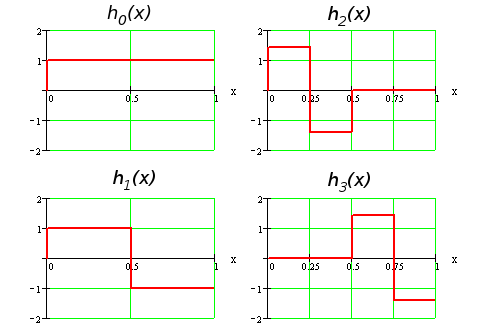
\includegraphics[width=0.95\textwidth]{../Graphics/Lectures-5-Haar_functions.png}
			\caption{Графики некоторых функций Хаара.}
		\end{subfigure}
	\end{figure}
	
	И так далее, образуя последовательность ортогональных ступенчатых функций. Любая функция, являющеаяся ступенчатой, может
	быть задана через линейную последовательность функций $h_0, \dots, h_n, \dots$.

\end{document}

    \documentclass[12pt]{article}

\usepackage[utf8]{inputenc}
\usepackage[russian]{babel}

\usepackage{amssymb}
\usepackage{amsmath}
\usepackage{amscd}
\usepackage{amsthm}
\usepackage{xcolor}

\usepackage{indentfirst}

%\usepackage{marginnote} % this is used for notes on the right margin --- \marginnote{\footnotesize txt}

\usepackage{mathtools} % for mathclap command

%\usepackage[normalem]{ulem} % for crossing text out - \sout

% Redefining \def is impossible. I tried, but it is impossible.
%\let\def_prev\def

%%%%%%%%%%%%%%%%%%%%%%%%%%%%%%%%%%%%%%%%%%%%%%%
%           MATH OPERATORS SPACING            %
%%%%%%%%%%%%%%%%%%%%%%%%%%%%%%%%%%%%%%%%%%%%%%%

\let\existstemp\exists
\let\foralltemp\forall
\renewcommand{\exists}{\: \existstemp \:}
\newcommand{\existsonly}{\: \existstemp ! \:}
\renewcommand{\forall}{\: \foralltemp \:}

%%%%%%%%%%%%%%%%%%%%%%%%%%%%%%%%%%%%%%%%%%%%%%%
%            COMMAND SHORTHANDS               %
%%%%%%%%%%%%%%%%%%%%%%%%%%%%%%%%%%%%%%%%%%%%%%%

\newcommand{\example}{{\itshape Пример. }}
\newcommand{\equals}{\Leftrightarrow}
\newcommand{\exc}{{\bfseries Упражнение. }}
\newcommand{\norm}[1]{\left\| #1 \right\|}
\newcommand{\scal}[2]{\left\langle #1, #2 \right\rangle}
\newcommand{\angular}[1]{\langle #1 \rangle}

\newcommand{\Sum}[2]{\underset{#1}{\overset{#2}{\sum}}}
\newcommand{\Int}[2]{\underset{#1}{\overset{#2}{\int}}}
\newcommand{\Ker}{\text{Ker}}

% Physicists' variant of dot product
\newcommand{\pscal}[2]{\, \langle #1 | #2 \rangle \,}
\newcommand{\bra}[1]{\, \langle #1 |}
\newcommand{\ket}[1]{| #1 \rangle \,}

\renewcommand{\leq}{\leqslant}
\renewcommand{\geq}{\geqslant}

%%%%%%%%%%%%%%%%%%%%%%%%%%%%%%%%%%%%%%%%%%%%%%%
%         THEOREM DEFINITION LINES            %
%%%%%%%%%%%%%%%%%%%%%%%%%%%%%%%%%%%%%%%%%%%%%%%

\newtheorem{lem}{Лемма}[section]
\newtheorem{note}{Замечание}[section]
\newtheorem{defi}{Определение}[section]
\newtheorem{theorem}{Теорема}[section]
\newtheorem{state}{Утверждение}[section] % statement

%%%%%%%%%%%%%%%%%%%%%%%%%%%%%%%%%%%%%%%%%%%%%%%
%             GRAPHICS INCLUSION              %
%%%%%%%%%%%%%%%%%%%%%%%%%%%%%%%%%%%%%%%%%%%%%%%

\usepackage{graphicx}

\graphicspath{{./Graphics/}}

%%%%%%%%%%%%%%%%%%%%%%%%%%%%%%%%%%%%%%%%%%%%%%%
%               DRAFT TEMPLATES               %
%%%%%%%%%%%%%%%%%%%%%%%%%%%%%%%%%%%%%%%%%%%%%%%

%\usepackage{marginnotes}
\newcommand{\todo}[1]{\marginpar{\color{red} \tiny #1}}

\begin{document}

\section{Операторы в гильбертовых пространствах}

	% Излишняя информация: и так очевидно, что многие обозначения не унифицированы.
	%Прежде чем начать изучение линейных операторов, стоит предупредить, что буквы, используемые нами для обозначения некоторых
	%классических операторов, могут не являться общепринятыми и отличаться от принятых в различной литературе по данному предмету.
	
	\begin{defi}
		Отображение $A$ из $M$ в $L$ назовём \textbf{линейным оператором}, если область определения оператора
		$D(A) \subset M$ и выполнены следующие условия:
		\begin{enumerate}
			\item $A(x + y) = Ax + Ay$
			\item $A(\alpha x) = \alpha A x$ 
		\end{enumerate}
		Обозначают $A : M \rightarrow L$.
	\end{defi}
	
	Впрочем, определение линейного оператора уже рассматривалось в курсе линейной алгебры. При рассмотрении линейных операторов в
	нашем курсе, будем предполагать, что $M$ и $L$ --- нормированные пространства. А если есть норма $\Rightarrow$ есть расстояние
	$\Rightarrow$ может быть определена непрерывность. Если $A$ непрерывно в $h_0$, пишут:
	
	$$ \forall \varepsilon > 0 \exists \delta > 0 : \forall h \: \norm{h - h_0} < \delta \Rightarrow \norm{Ah  Ah_0} 
	= \norm{A(h-h_0)} < \varepsilon $$
	Нетрудно видеть, что из непрерывности в точке следует непрерывность в нуле --- для этого нужно взять $h := h + h_0$. 
	Так же можно сделать для любой точки множества. Значит, $A$ непрерывна на всём множестве. Тогда, исходя из данного
	определения, получаем равномерную непрерывность для $A$.
	
	Приведём некоторые примеры линейных операторов:
	\begin{itemize}
		\item Тождественный оператор
		\item Нулевой оператор
		\item Оператор проектирования на замкнутое подпространство гильбертова пространства.
		\item $f(t) \rightarrow t \cdot f(t)$ в пространстве $\mathbb{L}_2 (0,1) \rightarrow \mathbb{L}_2 (0,1)$
		\item Оператор дифференцирования: $\text{\emph{D}}: \mathbb{L}_2 (0,1) \rightarrow \mathbb{L}_2 (0,1)$. Отметим также, что
		область определения этого оператора $D(\text{\emph{D}}) \neq \mathbb{L}_2 (0,1)$
		\item $f(x) \rightarrow \int_0^x f(t) dt$.
	\end{itemize}
	
	Для существования обратного оператора $A^{-1}$ нужно:
	\begin{enumerate}
		\item $A$ - инъективно.
		\item $D(A^{-1}) = $ образ прямого отображения
	\end{enumerate}
	В наших обозначениях, обратный оператор всегда определяет обратное отображение.

	\subsection{Ограниченный линейный оператор}	
	
	\begin{defi}
		Множество ограничено, если существет шар с центром в точке $O$, в котором содержится все множество.
	\end{defi}
	\begin{defi}
		Множество $M$ \textbf{ограничено}, если существет шар $B_r(a)$, в котором содержится все множество:
		$$ \exists a \in X \; \exists (r > 0) \; \forall x \in X (x \in M \Rightarrow \rho(a, x) < r) $$
	\end{defi}
	\begin{defi}
		Оператор $A: M \Rightarrow L$ называется \textbf{ограниченным}, если он переводит ограниченное множество
		в ограниченное.
	\end{defi}
	
	\begin{state}
		Линейный оператор ограничен $\equals$ он непрерывен.
	\end{state}
	\begin{proof}
		\textbf{Необходимость}. Если $A$ --- непрерывный оператор, то 
		$ \exists \delta : \norm{h} < \delta \Rightarrow \norm{Ah} < 1 $,
		откуда следует, что $\norm{h} < R$. 
		
		Рассмотрим вектор $x = \frac{\delta h}{R}$. В указанных условиях
		$\norm{x} < \frac{\delta}{R}$, откуда следует $\norm{Ax} < 1$ и, из линейности оператора и свойств нормы:

		$$\frac{\delta}{R} \cdot \norm {Ah} < 1$$
		
		Это означает, что отображение $A$ переводит все значения в шар радиуса $\frac{R}{\delta}$, значит
		$A$ --- ограниченный оператор. \\
		
		\textbf{Достаточность}. Аналогично доказательству необходимости. Если $A$ --- ограниченный оператор,
		то при $\norm{h} \leq 1$ получается $\norm{Ah} \leq R$. Возьмём шар радиуса $\frac{\varepsilon}{R}$
		и действуем так же, как в предыдущем доказательстве.
	\end{proof}
	
	\subsection{Норма линейного оператора}
	
	\begin{defi}
		\textbf{Нормой линейного оператора} $A$ называется выражение вида 
		$$\norm{A} \overset{df}{=} \underset{x \neq 0}{sup} \frac{\norm{Ax}}{\norm{x}}$$
	\end{defi}
	
	\begin{state}
		Линейный оператор ограничен $\equals$ его норма конечна.
	\end{state}
	\begin{proof}
		Распишем норму линейного оператора:
		$$
			\norm{A} \overset{df}{=} \underset{x \neq 0}{sup} \frac{\norm{Ax}}{\norm{x}} = 
			\underset{x \neq 0}{sup} \norm{A \frac{x}{\norm{x}}} =
			\underset{\norm{y} = 1}{sup} \norm{Ay} \leq
		$$
		$$
			\leq
			\underset{0 \leq \norm{y} \leq 1}{sup} \norm{Ay} \leq
			\underset{0 \leq \norm{y} \leq 1}{sup} \frac{\norm{Ay}}{\norm{y}} \leq
			\underset{y \neq 0}{sup} \frac{\norm{Ay}}{\norm{y}} =
			\norm{A}
		$$
		Так как все неравенства, приведенные здесь, были направлены в одну сторону,
		они обратятся в равенства. При этом, последнее равенство гарантирует, что
		оператор $A$ переведёт вектор $\norm{h} \leq r$ в замкнутый шар радиуса $\norm{A} \cdot r$.
		С другой стороны, при ограниченности оператора, его норма будет конечна, по приведённым
		выше равенствам.
	\end{proof}
	
	Сделаем также ещё одно замечание, исходящее из определения:
	$$ \frac{\norm{Ax}}{\norm{x}} \leq \norm{A} $$
	$$ \norm{Ax} \leq \norm{A} \cdot \norm{x} $$
	
	Мы в очередной раз что-то назвали нормой. Но {\color{gray}гуманно} верно ли это?
	
	\exc Для нормы линейного оператора выполнены все аксиомы нормы.
	% TODO: потом хотелось бы написать здесь доказательство и переписать это как "Утверждение".
	
	Также, остается упражнение по доказательству еще одного полезного свойства:
	
	\exc Доказать выполнение равенства $\norm{A} - \norm{B} \leq \norm{A-B}$.
	
	\begin{state}
		$$\norm{Ax} \leq k \norm{x} \Rightarrow \norm{A} \leq k$$
	\end{state}
	
	\begin{state}
		Для нормы композиции линейных операторов верно неравенство 
		$$\norm{A\cdot B} \leq \norm{A} \cdot \norm{B}$$
	\end{state}
	\begin{proof}
		$$ \norm{(AB)x} = \norm{A(Bx)} \leq \norm{A} \cdot \norm{Bx} \leq \norm{x} \cdot \norm{A} \cdot \norm{B} $$
		Отсюда 
		$$ \norm{AB} \leq \norm{A} \cdot \norm{B} $$
		что и требовалось доказать. \\
	\end{proof}
	
	\subsection{Оператор Гильберта-Шмидта}
	Рассмотрим пространства $\mathbb{L}_2(\mathbb{R}^n)$ и $\mathbb{L}_2(\mathbb{R}^k)$, а также функцию
	$$ k(x,y) \in \mathbb{L}_2(\mathbb{R}^{n+k}), x \in \mathbb{R}^n, y \in \mathbb{R}^k$$
	
	\begin{defi}
		\textbf{Оператором Гильберта-Шмидта} назовём оператор:
		$$ (Af)(t) \overset{df}{=} \underset{\mathbb{R}^k}{\int} k(t,y) f(y) dy $$
	\end{defi}
	
	Покажем, что функция $(Af)(t)$ определена почти для всех $t$. Пользуясь определением скалярного произведения в $\mathbb{L}_2$, 
	видим, что $\norm{(Af)(t)}^2 = (\scal{f}{k})^2 \leq \norm{f}^2 \cdot \underset{\text{на }\mathbb{R}^k}{\norm{k}^2}$
	
	$$ \norm{(Af)(t)}^2 \leq \underset{\mathbb{R}^k}{\int} |f(y)|^2 dy \cdot \underset{\mathbb{R}^k}{\int} |k(t,y)|^2 dy $$
	
	Проинтегрируем обе части выражения по множеству $\mathbb{R}^n$:
	
	$$ \Int{\mathbb{R}^n}{} \norm{(Af)(t)}^2 \, dt \leq \underset{\mathbb{R}^k}{\int} |f(y)|^2 \, dy 
	   \cdot \Int{\mathbb{R}^n}{} \Int{\mathbb{R}^k}{} |k(t,y)|^2 \, dt \, dy $$
	
	$k(t,y)$ почти всюду определена в $\mathbb{R}^k$, интегрируема
	в $\mathbb{R}^k$ по условию. Значит, по теореме Фубини можем переставить пределы интегрирования 
	и перейти к норме на $\mathbb{R}^n$.
	
	$$ \Int{\mathbb{R}^n}{} \norm{(Af)(t)}^2 \, dt \leq \norm{f}^2_{\mathbb{L}_2} \cdot \norm{k}^2_{\mathbb{L}_2} $$

	\lecture{6}

	Как известно, в конечномерном пространстве все нормы являются эквивалентными. Но это отнюдь не является верным для бесконечномерных
	пространств.
	
	\example \textit{(Неограниченного оператора)}. Оператор дифференцирования 
	$\frac{d}{dx} \mathbb{L}_2(0, 1) \rightarrow \mathbb{C}_2(0, 1)$ является неограниченным. 
	Достаточно рассмотреть $\norm{sin(nx)}_{\mathbb{L}_2} \leq 1$. При воздействии на синус оператором дифференцирования, получим
	$$|n \cdot cos(nx)| \geq n \cdot cos^2(nx) = n^2 \cdot \frac{1 + cos(2nx)}{2}$$
	Таким образом, легко увидеть неограниченность нормы $n \cdot cos(nx)$:
	\begin{align*}
		\norm{n \cdot cos(nx)}_{\mathbb{L}_2(0,1)}^2 
		&\geq \frac{n^2}{4} \Int{0}{1} \big(1 + 2 cos(2nx) + cos^2(2nx)\big) dx \geq \\
		&\geq \frac{n^2}{4} \Int{0}{1} \big(1 + 2 cos(2nx)\big) dx \geq \frac{n^2}{4} - 1
	\end{align*}
	При $n \rightarrow \infty$ этот образ не попадает в конечный шар, значит оператор $\frac{d}{dx}$ неограничен.
	
	% Доразобраться
	
	\todo{Уточнить формулировку.}
	\off{Скорее всего, здесь утверждается, что $\existsonly A_2$. Надо уточнить.}
	\begin{theorem} \label{th:limitedOperContinue}
		Рассмотрим линейный оператор $A_1 : E \rightarrow F$. Если выполнены следующие условия:
		\begin{enumerate}
			\item $F$ --- полное.
			\item $D(A_1) = E_1 \subset E_2$.
			\item $\overline{E}_1 \subset E_2$ (То есть $E_1$ плотно в $E_2$).
		\end{enumerate}
		То найдётся линейный оператор $A_2,\, D(A_2) = E_2$, такой, что: \\
		\todo{Быть может, здесь неравенство?}
		$\norm{A_2} \leq \norm{A_1}$ \\
		$A_2 \lims{E_1}{} = A_1$
	\end{theorem}
	
	\begin{proof}
		%   УБРАНО, ТАК КАК ИЗЛИШНЕ МНОГОСЛОВНО   %
		%Введём $x \in E_2, x_i \in E_1$. Пусть элементы $x_i$ образуют фундаментальную последовательность. Так как $E_1$ плотно в $E_2$,
		%то найдётся элемент $x \in E_2$, являющийся пределом последовательности $x_1, ..., x_n, ...$.
		Докажем по пунктам:
		\begin{itemize}
			\item $A_2 \lims{E_1}{} = A_1$ \\
			Положим $x_i \in E_1$, $\{x_n\}$ --- фундаментальная последовательность. Так как $E_1$ плотно в $E_2$, то
			$\lim x_n = x\in E_2$. Воздействуем на нашу последовательность оператором $A_1$.
			Последовательность $\{A_1 x_n\}$ останется фундаментальной. Так как $F$ --- полное пространство, 
			то любая фундаментальная последовательность в нём будет иметь предел:
		
			$$A_1x_n \rightarrow y \qquad y \in F$$
			Тогда, для любых $x \in E_2 \textbackslash E_1$, можно определить $A_2 x = y$. Осталось только 
			показать, что для предельных точек $A_2$ будет линейным оператором.
		
			Достаточно взять $z = \alpha x + \beta y$ и сходящуюся к нему последовательность $z_n = \alpha x_n + \beta y_n$.
			Воздействуя оператором $A_1$ на $z_n$, получаем выражение:
			$$A_1 z_n = \alpha A_1 x_n + \beta A_1 y_n$$
			В пределе, при $n \rightarrow \infty$, равенство преобразуется следующим образом:
			$$A_2 z = \alpha A_2 x + \beta A_2 y$$
			
			\off{По всей видимости, показали, что $A_2$ определяется однозначно и является линейным.}
			
			\item $\norm{A_2} \leq \norm{A_1}$ \\
			Другими словами, ограниченность оператора $A_1$ влечёт ограниченность оператора $A_2$. Рассмотрим следующее 
			неравенство:
			$$\norm{A_1 x_n} \leq \norm{A_1} \cdot \norm{x_n}$$
			В пределе $A_1 x_n \underset{n \rightarrow \infty}{\rightarrow} A_2 x$. Тогда
		
			$$\norm{A_2 x} \leq \norm{A_1} \cdot \norm{x}$$
		
			То есть $\norm{A_2} \leq \norm{A_1}$. С другой стороны 
			$\norm{A_2} = \underset{x\neq 0}{\sup} \frac{\norm{A_2x}}{\norm{x}} \geq \norm{A_1}$
			Таким образом, $\norm{A_1} = \norm{A_2}$.
		\end{itemize}
	\end{proof}
	
	Введём определение предела последовательности оператора. Стоит отметить, что в различной литературе данное определение может вводиться
	по-разному.
	
	\begin{defi}
		$A$ является \textbf{пределом} $A_n$, если:
		
		$$\forall x \in E, A_n x \underset{n \rightarrow \infty}{\rightarrow} A x$$
	\end{defi}
	В нормированных пространствах вводится еще один 
	важный термин:
	
	\begin{defi}
		Если для линейного оператора $A$ и последовательности линейных операторов $A_n$ определено соотношение:
		$$\norm{A_n - A} \rightarrow 0$$
		то $A_n$ \textbf{равномерно сходится} к $A$, что обозначается как $A_n \rightrightarrows A$.
	\end{defi}
	
	Легко показать, что равномерная сходимость всегда влечёт обычную. Действительно, рассмотрим
	$$\norm{A_n x - A x} \leq \norm{A_n - A} \cdot \norm{x} \rightarrow 0$$
	Отсюда следует $\forall x, A_n x \rightarrow A x$, что является определением сходимости линейных операторов.
	%\begin{state}
	%	Равномерная сходимость линейных операторов влечёт обычную.
	%\end{state}
	
	В приведённых выше рассуждениях есть одна неочевидная деталь --- предел последовательности элементов не обязательно должен лежать
	в том же множестве, что и элементы последовательности. Является ли $A$, как предел $A_n$ линейным оператором?
	
	\begin{state}
		Предел последовательности линейных операторов является линейным оператором.
	\end{state}
	\begin{proof}
		Проверим, обладает ли $A$ свойствами линейного оператора. Рассмотрим вектор $z = \alpha x + \beta y$. Тогда, пользуясь линейностью
		операторов из последовательности $A_n$:
		$$ A_n \cdot z \rightarrow A \cdot z $$
		$$ \alpha A_n x + \beta A_n y \rightarrow \alpha A x + \beta A y $$
		Значит, верно равенство $A(\alpha x + \beta y) = \alpha A x + \beta A y$ и $A$ является линейным оператором.
	\end{proof}
	
	Определить ограниченность оператора $A$, исходя из свойств последовательности $A_n$ намного сложнее, но легко установим следующий
	факт:
	\begin{state}
		Если $A_n \rightarrow A$ и $\forall n, \norm{A_n} \leq C$, где $C$ --- некоторая константа, то оператор $A$ является ограниченным.
	\end{state} 
	\begin{proof}
		Очевидно. {\color{gray}Sorry, но я и так умаялся предыдущее доказательство писать, а оно тоже очевидное.}
	\end{proof}

	\example $P_n : l_2 \rightarrow l_2$ --- оператор проектирования на n-мерное подпространство.
	$$P_n : (x_1, \dots , x_n, x_{n+1}, \dots) \longmapsto (x_1, \dots, x_n, 0, 0, 0, \dots)$$
	Рассматривая свойства пространства $l_2$, легко понять, что $P_n \rightarrow I$. Действительно, так как $x_n$ --- элементы 
	сходящегося ряда, то норма <<хвоста>> этого ряда будет стремиться к нулю.
	%\marginnote{\footnotesize I --- тождественный оператор}[-1.5cm]
	Но, в то же время, равномерной сходимости не достигается: $\norm{P_n - I} = 1$. Следовательно, обычная сходимость не влечёт
	равномерную.
	
	\exc Пусть $A_n \rightrightarrows A, B_n \rightrightarrows B$. Доказать $A_n B_n \rightrightarrows A B$. 
	(Разумеется, доказывается данное утверждение в предположении, что композиция $A B$ существует, то есть совпадают область определения
	A и множество значений B.)
	
	\begin{state}
		Рассмотрим последовательность $A_n : E \rightarrow F$. Утверждается, что, если $F$ --- полное, то пространство 
		ограниченных линейных операторов $\{A_n\}$ образует полное нормированное пространство.
	\end{state}
	\begin{proof}
		Возьмём $A_n$ --- фундаментальную последовательность, тогда $\norm{A_n - A_m} \rightarrow 0$, отсюда следует, что 
		$A_n \cdot x$ --- фундаментальная последовательность и, так как $F$ --- полное множество, она имеет предел, который
		мы обозначим за $A \cdot x$ ($\forall x A_n \cdot x \rightarrow A \cdot x$).
		
		\textbf{Линейность.} Ранее уже было доказано, что предел последовательности линейных операторов также является линейным
		оператором.
		
		\textbf{Ограниченность.} Так как последовательность является фундаментальной, можем ограничить норму разности её элементов 
		с достаточно большими номерами константой.
		$$\forall n,m > N,\,\,\norm{A_n - A_m} \leq 1$$
		Тогда, применяя неравенство треугольника, легко приходим к доказательству ограниченности оператора:
		$$\norm{A_n} \leq 1 + \norm{A_m}$$
		
		\textbf{Равномерная сходимость.} По определению фундаментальной последовательности:
		$$
			\norm{A_n - A_m} \rightarrow 0 \overset{df}{\equals} 
			\forall \varepsilon > 0\, \exists N_0\, \forall m, n \geq N_0 \:\: \norm{A_n - A_m} < \varepsilon
		$$
		В силу $A_n \rightrightarrows A$, получаем, в таких же обозначениях:
		$$ \norm{A_n - A} \leq \varepsilon $$
		Данное неравенство при $\varepsilon \rightarrow 0$ является определением равномерной сходимости.
		
		Таким образом, $\{A_n\}$ обладает всеми свойствами, нужными для того, чтобы пространство являлось полным, что и требовалось 
		доказать.
	\end{proof}
	
	\begin{defi}
		Если для полного пространства $F$ и операторов $A_n : E \rightarrow F$ имеет место предельное соотношение
		$$\Sum{n=1}{N} A_n \underset{N \rightarrow \infty}{\rightarrow} A,$$
		то оператор $A = \Sum{n=1}{\infty} A_n$ называют \textbf{операторным рядом}.
	\end{defi}
	
	Определим для подобного ряда критерий Коши (критерий сходимости фундаментальной последовательности):
	$$\forall \varepsilon > 0 \exists N(\varepsilon) m > n > N(\varepsilon) \norm{ \Sum{n}{m} A_i } < \varepsilon$$
	
	Операторный ряд является одним из способов построения функции от операторов. Но данным способом могут быть выражены только 
	аналитические функции.
	
	\example Пусть $A$ --- ограниченный линейный оператор. Тогда ряд 
	$$\Sum{n = 0}{\infty} \frac{A^n}{n!}$$
	сходится, так как $\norm{A^n} \leq \norm{A}^n$, а ряд $\Sum{n=0}{\infty} \frac{\norm{A}^n}{n!}$ ничем не отличается от ряда
	$\Sum{n=0}{\infty} \frac{t^n}{n!}$, обладающего радиусом сходимости $R = \infty$.
	
	\subsection{Обратный оператор}
	
	Чтобы существовало обратное отображение $A^{-1}$, необходима инъективность оператора $A$. Более формально это записывается так: \\
	Пусть $E : A \rightarrow F$ и $A$ --- инъективен $\Rightarrow \exists A^{-1}, D(A^{-1}) = Im(A)$.
	
	\begin{state}
		$A^{-1}$ аддитивен и линеен.
	\end{state}
	\begin{proof}
		\textbf{Аддитивность.} Рассмотрим вектора $y \in Im(A), z \in Im(A)$, тогда по линейности $A$, $y + z \in Im(A)$.
		Определим вектор $x$:
		$$x = A^{-1}(y + z) - A^{-1} y - A^{-1} z$$
		Воздействуем на него оператором A, учитывая, что $A A^{-1} = I$.
		$$Ax = I(y + z) - I y - I z = 0$$
		Таким образом, из линейности оператора $A$, $x = 0$, что доказывает аддитивность обратного оператора.
		
		\textbf{Однородность.} Опять же, рассмотрим $y \in Im(A)$ и определим вектор $x$:
		$$ x = A^{-1}(\lambda y) - \lambda A^{-1} y $$
		$$ Ax = \lambda y - \lambda y = 0 $$
		Следовательно, $x = 0$, поэтому $A^{-1}$ однородно.
		
		Доказаны аддитивность и однородность $\Rightarrow$ оператор $A^{-1}$ линеен.
	\end{proof}
	
	Ограниченность оператора $A$ отнюдь не влечёт ограниченность $A^{-1}$.
	
	\begin{theorem}
		(Без доказательства) Если $A$ --- линеен, ограничен и отображает полное нормированное пространство на полное нормированное
		пространство, то $\exists A^{-1}$ --- линейный и ограниченный оператор.
	\end{theorem}
	
	Пусть $A$ --- линейный оператор и $$\exists m > 0 : \forall x \norm {Ax} \geq m \cdot \norm{x}$$
	Это будет означать, что $A$ --- инъективный оператор, так как
	$$\norm{A(x-y)} \geq m \cdot \norm{x - y}$$
	Из этого неравенства следует, что, если $Ax = Ay$, то $x = y$. И, разумеется, инъективность оператора будет означать его
	обратимость.
	
	В таких условиях, оператор $A^{-1}$ будет ограниченным:
	$$ x = A^{-1} y $$
	$$ \norm{A^{-1} y} \leq \frac{1}{m} \norm{y} $$
	И это, в силу определения нормы оператора, означает $$\norm{A} \leq \frac{1}{m}$$
	
	\begin{theorem}
		Пусть $F$ --- полное пространство, $A : F \rightarrow F$ --- линейный оператор, $\norm{A} \leq 1$.
		Тогда оператор $I_F - A$ является обратимым, причём обратный оператор определяется как:
		$$
			(I_F - A)^{-1} = \Sum{0}{\infty} A^n
		$$
	\end{theorem}
	Стоит отметить, что ряд $\Sum{0}{\infty} A^n$ будет сходиться, так как $\norm{A} \leq 1$. Более того, сумма этого ряда определяется
	как сумма бесконечно убывающей геометрической прогрессии.
	\begin{proof}
		Умножим $(I_F - A)$ на частичную сумму ряда $\Sum{0}{N} A^n$:
		$$ (\Sum{0}{N} A^n ) \cdot (I_F - A) = I_F - A^{N+1} \rightarrow I_F $$
		Взяв $N \rightarrow \infty$ превратим предел в равенство; умножим обе части уравнения на $(I_F - A)^{-1}$. Получаем
		$$ \Sum{0}{\infty} A^n = (I_F - A)^{-1} $$
		что совпадает с формулой, указанной в теореме.
	\end{proof}
	
	\begin{state}
		A --- обратим, $\Delta$ --- ограниченный оператор, $\norm{\Delta} \leq \frac{1}{\norm{A^{-1}}}$, тогда оператор 
		$A + \Delta$ будет обратимым.
	\end{state}
	\begin{proof}
		Вынесем $A$ за скобки:
		$$ A + \Delta = A \cdot \underbrace{(I + A^{-1} \cdot \Delta)}_
		   { \mathclap{\text{Обратимо по предыдущей теореме.}} } 
		$$
	\end{proof}
	
	\subsection{Спектр линейного оператора}
	
	Рассмотрим $A : F \rightarrow F$:%, $F$ --- плотное пространство.
	$$(A - \lambda \cdot I) = \lambda \cdot (\frac{A}{\lambda	} - I)$$
	Как видно из ранее приведённых теорем, оператор $(A - \lambda \cdot I)$ будет обратимым при достаточно больших значениях $\lambda$.
	
	Запишем все группы $\lambda$, определяемые свойствами оператора $(A - \lambda \cdot I)$
	
	\begin{center}
		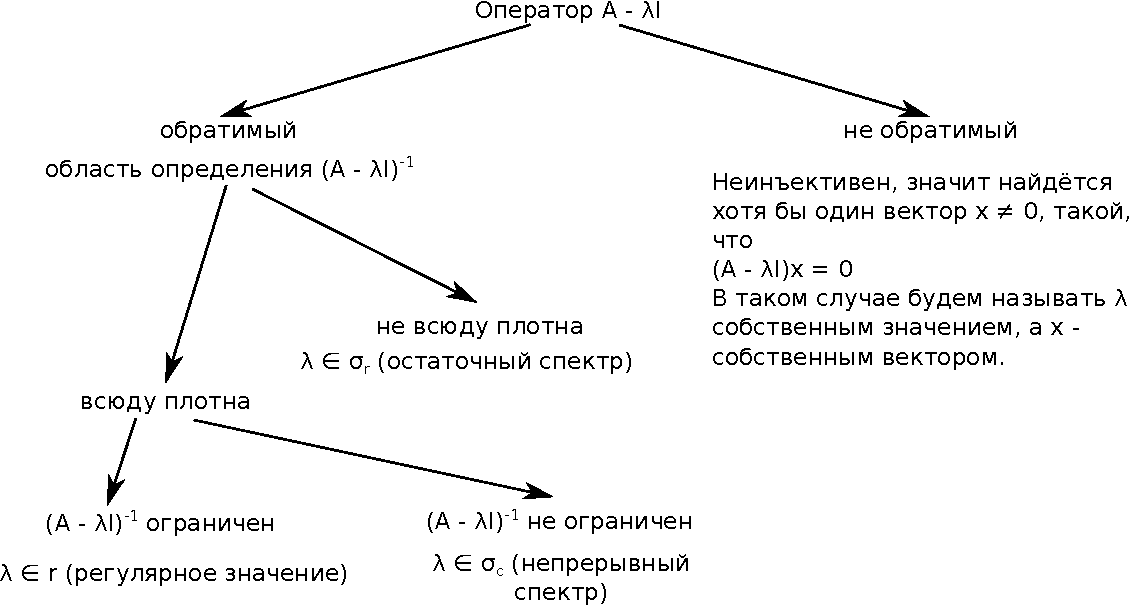
\includegraphics[width=1.0\linewidth]{../Graphics/Lectures-6-spectrum_scheme.pdf}\\
	\end{center}
	
	Для каждого $\lambda \in r(A)$ определяется ограниченный, с всюду плотной областью определения оператор
	$$ R_{\lambda} = (A - \lambda I)^{-1}$$
	Где $R_{\lambda}$ называется \textbf{резольвентным оператором}. \\
	Также отметим равенство, верное для любого линейного оператора:
	$$
		\overbrace{r(A)}^{ \mathclap{\text{Регулярные значения $A$}} } \cup 
		\underbrace{\sigma_1 (A) \cup \sigma_2 (A) \cup \sigma_3 (A)}_{\text{Спектр $A$}} = 
		r(A) \cup \sigma(A) = \mathbb{C}
	$$

	\lecture{7}

	% В конспекте упущено упоминание того, что было в прошлой лекции.

	%\subsection{Спектр и регулярные значения линейного оператора}
	
	На прошлой лекции был рассмотрен оператор $(A - \lambda I)$, и классификация значений $\lambda$, определяющаяся свойствами этого 
	оператора. Для удобства, в дальнейшем будем использовать обозначение $A_{\lambda}$.
	
	\begin{state}
		Множество регулярных значений $r(A)$ оператора $A$ является открытым.
	\end{state}
	\begin{proof}
		Ранее было доказано, что оператор $(A + \Delta)$ обратим, если $\norm{\Delta} \leq \frac{1}{\norm{A^{-1}}}$ 
		и $A$ является обратимым оператором. Тогда, если $\lambda \in r(A)$, то оператор
		$$ (A - \lambda I) - \mu I $$
		является обратимым для малых $\mu$. Этим доказывается открытость множества $r(A)$.
	\end{proof}
	С другой стороны, для любого линейного оператора верно
	$$
		\overbrace{r(A)}^{ \mathclap{\text{Регулярные значения $A$}} } \cup 
		\underbrace{\sigma_1 (A) \cup \sigma_2 (A) \cup \sigma_3 (A)}_{\text{Спектр $A$}} = 
		r(A) \cup \sigma(A) = \mathbb{C}
	$$
	Данное равенство означает, что, в силу открытости $r(A)$, \textbf{спектр линейного оператора --- замкнутое множество}.
	
	\subsection*
	{
		Сопряжённые гильбертовы пространства. \\
		Основная\footnote{В рамках нашего курса.} теорема гильбертова пространства.
	}
	
	\begin{defi}
		Пусть $E$ --- банахово пространство. Тогда $E'$ будем называть 
		\textbf{пространством непрерывных линейных функционалов из $E$ в $\mathbb{C}$} 
		или \textbf{пространством, сопряжённым к $E$}.
	\end{defi}
	
	Данное определение очень похоже на определение обобщённых функций, введённых в предыдущем курсе функционального анализа. 
	Единственным отличием является то, что теперь функционалы задаются в нормированном пространстве, в отличие от
	обобщённых функций, где топология задавалась исключительно понятием сходимости
	\footnote
	{
		Строго говоря, топология пространства обобщённых функций также может определяться множеством 
		полунорм --- норм, которые могут равняться нулю на ненулевых элементах. Но эта информация выходит
		за рамки данного курса.
	}
	.
	
	Как и для линейных операторов, линейный функционал непрерывен тогда и только тогда, когда он ограничен. Единственное отличие
	между ними заключается в том, что линейные функционалы обладают фиксированным множеством прибытия.
	
	Преимущественно будем использовать $H'$ --- пространство, сопряжённое гильбертову.
	
	Рассмотрим линейный функционал $l: H \rightarrow \mathbb{C}$. Для него определено понятие ядра:
	$$\Ker(l) = \{ h \in H | l \angular{h} = 0\}$$
	В общем случае непрерывного линейного функционала, ядро обладает следующими свойствами:
	\begin{itemize}
		\item $\Ker$ --- не пустое множество. \\
		(В силу линейности в нём обязательно лежит $h = 0$)
		\item $\Ker$ --- линейное подпространство. \\
		(В силу линейности функционала)
		\item $\Ker$ --- замкнутое подпространство. \\
		(Пусть $x_n \in \Ker(l)$, $x_n \rightarrow x_0 \Rightarrow l\angular{x_n} \rightarrow l\angular{x_0}$)
	\end{itemize}
	
	\exc Доказать, что если ядро линейного функционала $f$ замкнуто, то $f$ ограничен.
	
	% TODO: Разобрать, как поставить, чтобы была не теорема 4.1, а теорема Рисса.
	\begin{theorem} 
		Пусть $l: H \rightarrow \mathbb{C}$ --- линейный ограниченнный функционал, тогда
		\begin{enumerate}
			\item $\existsonly h_l \in H$, такой, что 
			$$\forall h \in H, l \angular{h} = \scal{h}{h_l}$$
			\item $\forall g \in H$, формула (markme!) определяет линейный непрерывный функционал
			$$f\angular{h} \rightarrow \mathbb{C}$$
			$$f\angular{h} = \scal{h}{g}$$
		\end{enumerate}
	\end{theorem}
	\begin{proof}
		Докажем по порядку приведённые пункты теоремы:
		\begin{enumerate}
			\item Обозначим $G = \Ker(l)$. В таком случае, возможны два варианта:
			\begin{enumerate}
				\item Ядро совпадает с гильбертовым пространством: $(G = H)$. \\
				Данное равенство будет означать, что любой вектор пространства обращается функционалом в ноль.
				Следовательно, $h_l = 0$ будет единственным подходящим решением.
				\item Ядро не совпадает с гильбертовым пространством: $G \neq H$. \\
				Так как $G$ --- замкнутое подпространство, то его ортогональное дополнение $G^{\perp} \neq \{0\}$
				
				Тогда можно взять вектор $h_0 \in G^{\perp}, h_0 \neq 0$. Взяв произвольный $h \in H$, рассмотрим вектор
				\begin{equation} \label{eq:RissVector}
					(l\angular{h}) h_0 - (l\angular{h_0}) h
				\end{equation}
				Несложно показать, что вектор \eqref{eq:RissVector} лежит в G. Действительно,
				$$
					l\angular{(l\angular{h}) h_0 - (l\angular{h_0}) h} 
					= l\angular{h}l\angular{h_0} - l\angular{h_0}l\angular{h} = 0
				$$
				Теперь рассмотрим скалярное произведение векторов \eqref{eq:RissVector} и $h_0$:
				$$
					(l\angular{h}) \cdot \norm{h_0}^2 - (l\angular{h_0}) \cdot \scal{h}{h_0} = 0
				$$
				Откуда в результате нехитрых преобразований получается 
				\begin{equation} \label{eq:hlvector}
					h_l = \frac{\overline{l\angular{h_0}}}{\norm{h_0}^2} \cdot h_0
				\end{equation}
			\end{enumerate}
			Докажем единственность полученного $h_l$. Предположим, что это не так и существуют два вектора $h'$ и $h''$, таких, что 
			$$l\angular{h} = \scal{h}{h'} = \scal{h}{h''}$$
			Тогда будет верно
			\begin{eqnarray*}
				\scal{h}{h'} = \scal{h}{h''} \\
				\scal{h}{(h' - h'')} = 0
			\end{eqnarray*}
			Так как данное равенство верно для любых $h$, возьмём $h = h' - h''$. Получим $\norm{h'-h''}^2 = 0$, откуда следует
			$h' = h''$, что и требовалось доказать.
			
			{\footnotesize
				Единственность $h_l$ позволяет судить о размерности $G^{\perp}$.
				Так как \eqref{eq:hlvector} выполнено для всех $h_0 \in G^{\perp}$, вектор $h_l$ параллелен всем $h_0$, 
				что возможно лишь при $\dim{G^{\perp}} = 1$ ($\dim{G^{\perp}} \neq 0$ по предположению доказательства).
			}
			
			\item Рассмотрим функцию $f$, такую, что $f(h) = \scal{h}{g}$. В силу свойств скалярного произведения, 
			$f(h)$ --- линейный функционал, который, в силу неравенства Шварца, будет ограниченным:
			\begin{equation} \label{eq:BoundedProof}
				|f(h)| \leq \norm{h} \cdot \norm{g} \Rightarrow \norm{f} \leq \norm{g}
			\end{equation}
			Подставим $h = g$ в функцию $f(h)$. Получим
			$$|f(g)| = \norm{g}^2$$
			Так как норма оператора, определяется как $\sup \frac{f(h)}{\norm{h}}$, то 
			$$\norm{f} \geq \norm{g}$$
			Рассматривая данное неравенство вместе с первым неравенством из \eqref{eq:BoundedProof}, получаем 
			$$ \norm{f} = \norm{g} $$
			
			Или, в обозначениях предыдущего пункта, $\norm{h_l} = \norm{l}$.
			
			{\footnotesize
				При этом, из $\dim{G^{\perp}} \leq 1$, получим $f(h) = C(h) \cdot \norm{h}^2$, где $C(h)$ --- коэффициент из 
				\eqref{eq:hlvector}. В результате, линейный функционал для любого вектора ограничен как 
				$|f(h)| \leq C \cdot \norm{h^2}$
			}
		\end{enumerate}
	\end{proof}
	
	\begin{note}
		Теорема Рисса устанавливает биекцию $H' \leftrightarrow H$.
	\end{note}
	\begin{proof}
		Рассмотрим формулу $l_1\angular{h} = \scal{h}{h_{l_1}}, h \in H$. Для неё верны следующие
		свойства:
		\begin{itemize}
			\item Оператору $l_1 + l_2$ соответствует вектор $h_{l_1+l_2}$.
			\item Для $\alpha l_1, \alpha \in \mathbb{C}$ $h_{\alpha l_1} = \bar{\alpha} h_l$
		\end{itemize}
	\end{proof}
	
	Введя второе сопряжённое пространство $H''$, увидим следующую связь:
	$$H'' \leftrightarrow H' \leftrightarrow H$$
	При этом, здесь $\leftrightarrow$ обозначает эрмитов изоморфизм, когда 
	$h_{\alpha l} = \bar{\alpha} h_l$. % Кривовато выводит, надо будет подумать над правильной вёрсткой.
	Видим, что $H$ и $H''$ связаны обычным изоморфизмом, то есть $h_{\alpha l} = \alpha h_l$.
	% Гильбертов также называется сопряженно линейным, обычный --- канонический.
	
	\subsection{Бра- и кет-векторы.}
	Теорема Рисса отождествляет линейный ограниченный функционал с линейными вектороами гильбертова пространства.
	Но мы привыкли к префиксной записи (а здесь $h_l$, заменяющий функционал, пишется справа), поэтому у физиков
	скалярное произведение линейно по второму аргументу. На текущий и следующий разделы мы тоже <<перейдём в эту веру>>.
	
	$$\scal{f}{g} \overset{df}{=} \pscal{g}{f}$$
	Которое будем называть физическим скалярным произведением, линейным по $g$. Но мы пойдём дальше --- представив
	$\pscal{g}{f} = \bra{g} \ket{f}$, разорвём скалярное произведение. Таким образом, приходим к следующему формализму: \\
	\begin{tabular}{l c r}
		$\bra{g}$ & --- & бра-вектор \\
		$\ket{f}$ & --- & кет-вектор \\
	\end{tabular}
	(от английского \textit{bracket} --- скобки)
	
	Авторство данного формализма принадлежит Дираку, который ввёл её для описания квантовых состояний.
	
	Пусть $e_n$ --- гильбертов базис, тогда каждый вектор совпадает с суммой своего ряда Фурье:
	$$ \forall h,\quad h = \sum \alpha_n e_n,\: \alpha_n = \scal{h}{e_n} $$
	Для гильбертова базиса, запишем сначала кет-вектор, потом бра-вектор:
	$$ \ket{e_n} \bra{e_n} $$
	$$ \sum \ket{e_n} \pscal{e_n}{h_n} = \sum \ket{e_n} \alpha_n = h $$
	Так как подобное преобразование переводит $h$ в $h$, результат очевиден:
	$$ \sum \ket{e_n} \bra{e_n} = I_H $$
	
	\subsection{Операторная функция Грина}
	
	Рассмотрим линейный оператор $A : H \rightarrow H$ с собственными числами $\lambda_i$ и собственными векторами $e_i$,
	$$A e_i = \lambda_i e_i$$
	Причём $\{e_i\}$ --- гильбертов базис в $H$.
	
	Теперь рассмотрим $\lambda \neq \lambda_i$ и решим уравнение
	$$ Ax - \lambda x = y $$
	Кет-вектор $\ket{x}$ может быть записан как сумма ряда Фурье:
	$$ \ket{x} = \sum x_n \ket{e_n} $$
	Рассмотрим $A \ket{x} = \sum \lambda_n x_b \ket{e_n}$. Вычтем $\lambda \ket{x}$ из каждой стороны:
	\begin{equation} \label{ketEq}
		A\ket{x} - \lambda\ket{x} = \sum (\lambda_n - \lambda) \cdot x_ \ket{e_n} = \ket{y}
	\end{equation}
	
	Домножим \eqref{ketEq} на бра-вектор $\bra{e_m}$ слева. Тогда, так как $\{e_i\}$ --- гильбертов базис,
	то $(\lambda_n - \lambda) x_n = \pscal{e_m}{y}$.
	$$ x_m = \frac{1}{\lambda_m - \lambda} \cdot \scal{e_m}{y} $$
	Умножая полученное выражение на $\ket{e_m}$, получаем
	$$ \sum_n x_n \ket{e_m} = \sum_m \frac{\ket{e_m}}{\lambda_m - \lambda} \pscal{e_m}{y} $$
	Таким образом, получили выражение исходного вектора через результат оператора:
	$$ \ket{x} = \sum_m \frac{\ket{e_m} \bra{e_m}}{\lambda_m - \lambda} \ket{y} $$
	\begin{equation} \label{greenFunction}
		A^{-1}_{\lambda} = \sum_m \frac{\ket{e_m} \bra{e_m}}{\lambda_m - \lambda}
	\end{equation}
	Равенство \eqref{greenFunction} определяет резоленту и называется \textbf{операторной функцией Грина}.
	
	Выводя данную функцию, мы поступали как физики: не проверяли законность деления и суммирования. Но главное одно:
	результат получен.
	
	\subsection{Сопряжённые операторы}
	Рассмотрим $A: E \rightarrow F$, пусть $f\in F'$ --- линейный ограниченный функционал.
	В таком случае виден функционал $f\angular{A} \in E'$.
	
	\begin{defi} \label{def:adjointOp}
		Для линейного оператора $A: G \rightarrow F$, оператор \\$A^{*}: F' \rightarrow G'$ 
		называется \textbf{сопряжённым оператором}, если он выполняет отображение $f \mapsto g$,
		где $f \in F'$ и $g \in G'$ --- линейные функционалы, и $\forall h \in G, \: g\angular{h} = f\angular{Ah}$
	\end{defi}
	
	Тогда рассмотрим линейный ограниченный оператор $A: H_1 \rightarrow H_2 $, 
	где $H_1, H_2$ --- гильбертовы пространства. Тогда, по теореме Рисса, можем ввести
	непрерывный линейный функционал 
	$$l_2 \in H_2', \: l_2 = \scal{\:}{h_{l_2}}$$
	В таком случае, действием такого функционала на вектор $h_1 \in H_1$ будет
	$$l_2 \angular{h_1} = \scal{A h_1}{h_{l_2}}$$
	Поставим вектору $h_{l_2} \in H_2$ вектор $h_{l_1} \in H_1$, то есть
	$$ l_2 \angular{h_1} = \scal{h_1}{h_{l_1}} = \scal{h_1}{A^{*} h_{l_2}}$$
	
	По определению сопряжённого оператора, для любых $h_1 \in H_1$, $h_2 \in H_2$, будет выполняться равевнство
	\begin{equation} \label{eq:adjointOp}
		\scal{A h_1}{h_2} = \scal{h_1}{A^{*} h_2}
	\end{equation}
	
	{ \color{gray}
		Если на экзамене про сопряжённый оператор будет сказано только \eqref{eq:adjointOp}, полным <<криминалом>> это не будет.
		Тем не менее, для ответа на отличную оценку желательно сказать определение (\ref{def:adjointOp}).
	}
	%%% То, что я не знаю куда запихать:
	% Гильбертов базис, в данном курсе является ортонормированной системой 
	% векоторов, которая полна.
	% В гильбертовом базисе разложение вектора по базису --- сумма ряда, в силу бесконечномерности.
	% Гильбертов базис не во всех книгах является ортонормированным.

	\lecture{8}

	В ходе прошлой лекции была доказана теорема Рисса, дающая представление о том, как выглядит функционал в гильбертовом пространстве.
	
	{\color{gray}
		Здесь следует повторная формулировка теоремы Рисса.
	}
	
	Пусть существует функционал $f \in H_2'$. Тогда, по теореме Рисса, ему соответствует вектор $h_f \in H_2$, такой, что 
	$$\forall h \in H_2, \: f(h) = \scal{h}{h_f}$$
	Определим линейный оператор $A : H_1 \rightarrow H_2$. Для $x \in H_1$: 
	$$f(Ax) = \scal{Ax}{h_f}$$
	По теореме Рисса, найдётся единственный вектор $h_g$, такой, что 
	$$f(Ax) = g(x) = \scal{x}{h_g}$$
	И векторы $h_f$ и $h_g$ будут связаны соотношением:
	$$h_g = A^{*}h_f$$
	Таким образом, вводится понятие \textbf{сопряжённого оператора}.

	% Коряво, стоит потом глянуть в литературе.
	Теорема Рисса также приводит нас к доказательству ещё одного важного свойства:
	\begin{state}
		%Пусть функционал $f_1: L \rightarrow \mathbb{C}$ линеен, ограничен и его область определения $D(f_1) = L$,
		%причём $L \neq H$ --- всему гильбертову пространству. Тогда найдётся линейный ограниченный функционал 
		%$f: H \rightarrow \mathbb{C}$, определённый на всём пространстве и $f|_{L} = f_1$.
		Пусть функционал $f$ линеен и ограничен. Если область определения этого функционала $D(f) \subset H$, 
		где $H$ --- гильбертово пространство, то функционал $f$ можно расширить на всё пространство $H$.
	\end{state}
	\begin{proof}
		Ранее было доказано, что линейный ограниченный оператор можно продолжить на замыкание его области определения 
		(Теорема (\ref{th:limitedOperContinue})). Тогда, даже если $\overline{D(f)} \neq H$, всё равно $\overline{D(f)}$ --- гильбертово 
		пространство.
		А это значит, что, по теореме Рисса, мы можем сопоставить ему вектор $h_f \in \overline{D(f)} \subset H$, такой, что 
		$f(h) = \scal{h}{h_f}$. Но, так как $h_f \in H$, то $\scal{h}{h_f}$ определено на всём пространстве $H$. \\
	\end{proof}
	
	Благодаря этому утверждению, в дальнейшем функционалы можно считать определёнными на всём гильбертовом пространстве.
	
	\subsubsection{Свойства сопряжённого оператора}
	
	\begin{enumerate}
		\item Линейность
		\begin{align*}
			\underline{ \scal{h_1}{A^{*}\angular{\alpha h + \beta g}} } &= \scal{Ah_1}{\alpha h + \beta g} = 
			\bar{\alpha}\scal{Ah_1}{h} \bar{\beta}\scal{Ah_1}{g} = \\
			&= \scal{h_1}{\alpha A^{*} h} + \scal{h_1}{\beta A^{*} g} = 
			\underline{ \scal{h_1}{\alpha A^{*} h + \beta A^{*} g} }
		\end{align*}
		Так как подчёркнутые выражения равны для любых $h_1$, будет выполнено равенство
		$$A^{*}\angular{\alpha h + \beta g} = \alpha A^{*} h + \beta A^{*} g$$
		
		\item Ограниченность \label{bounded}
		
		Рассмотрим скалярное произведение $\scal{h}{A^{*}g}$: 
		$$\scal{h}{A^{*}g} = \scal{Ah}{g} \leq \norm{Ah}\cdot\norm{g} \leq \norm{A}\cdot\norm{h}\cdot\norm{g}$$
		Теперь, поставим $h = A^{*}g$:
		\begin{gather*}
			\norm{A^{*}g}^2 \leq \norm{A}\cdot\norm{A^{*}g}\cdot\norm{g} \\
			\norm{A^{*}g} \leq \norm{A}\cdot\norm{g} \\
			\dfrac{\norm{A^{*}g}}{\norm{g}} \leq \norm{A}
		\end{gather*}
		Вспомним определение нормы оператора: $\norm{A^{*}} = \underset{g \neq 0}{\sup} \frac{\norm{A^{*}g}}{\norm{g}}$. Тогда очевидно
		$\norm{A^{*}} \leq \norm{A}$.
		
		\item $(\alpha A + \beta B)^{*} = (\bar{\alpha}A^{*} + \bar{\beta}B^{*})$ \label{conjlin}
		\begin{align*}
			\scal{(\alpha A + \beta B)h}{g} &= \scal{h}{(\alpha A + \beta B)^{*}g} \\
			\scal{(\alpha A + \beta B)h}{g} &= \alpha\scal{Ah}{g} + \beta\scal{Bh}{g} 
			= \alpha\scal{h}{A^{*}g} + \beta \scal{h}{B^{*}g} = \\
			&= \scal{h}{(\bar{\alpha}A^{*} + \bar{\beta}B^{*})g}
		\end{align*}
		Таким образом, $\forall h\: \scal{h}{(\alpha A + \beta B)^{*}g} = \scal{h}{(\bar{\alpha}A^{*} + \bar{\beta}B^{*})g}$, 
		следовательно $(\alpha A + \beta B)^{*} = (\bar{\alpha}A^{*} + \bar{\beta}B^{*})$ \\
		
		\item $(BA)^{*} = A^{*}B^{*}$
		\todo{Использовать \textbf{tikz-cd}, в нём лучше такие вещи делать.}
		$$
		\begin{CD}
			\scal{BAh}{g} @. = @. \scal{h}{(BA^{*})g} \\
				@| \\
			\scal{Ah}{B^{*}g} @. = @. \scal{h}{A^{*}B^{*}g}
		\end{CD}
		$$
		
		Отсюда $\scal{h}{A^{*}B^{*}g} = \scal{h}{(BA^{*})g}$ и $(BA^{*}) = A^{*}B^{*}$.
		
		{\Large(}Это свойство доказывает $(A^n)^{*} = (A^{*})^n,\, n \in \mathbb{N}$. ($B=A^{n-1}$){\Large)} \\
		
		\item $I^{*} = I$
		$$
		\left.
		\begin{CD}
			\scal{Ih}{g} @. = @. \scal{h}{I^{*}g} \\
				@| \\
			\scal{h}{g} @. = @. \scal{h}{Ig}
		\end{CD}
		\right\} \Rightarrow I = I^{*}
		$$
		
		\item $(A^{*})^{*} = A$ \label{doubleconj}
		
		Для оператора $A: H_1 \rightarrow H_2$, рассмотрим $h \in H_1$, $g \in H_2$:
		$$
			\scal{g}{(A^{*})^{*}h} = \scal{A^{*}g}{h} = \overline{\scal{h}{A^{*}g}} = 
			\overline{\scal{Ah}{g}} = \scal{g}{Ah}
		$$
		Таким образом, $\forall g,h \: \scal{g}{(A^{*})^{*}h} = \scal{g}{Ah} \Rightarrow (A^{*})^{*} = A$
		
		\item $\norm{A} = \norm{A^{*}}$
		
		Очевидно по свойствам (\ref{bounded}) и (\ref{doubleconj}):
		
		$$
		\left.
		\begin{aligned}
			\norm{A^{*}} &\leq \norm{A} \\
			\norm{A} &\leq \norm{A^{*}}
		\end{aligned}
		\right\}
		\Rightarrow \norm{A} = \norm{A^{*}}
		$$
		
		\item Если матрица $A$ обратима, то $(A^{-1})^{*} = (A^{*})^{-1}$.
		
		\exc Доказать это свойство. \\
		{\Large(}Это также автоматически докажет $(A^n)^{*} = (A^{*})^n,\, n \in \mathbb{Z}${\Large)}
	\end{enumerate}
	
	\subsubsection{Самосопряжённый оператор}
	
	\begin{defi}
		Оператор $A : H \rightarrow H$ называется \textbf{самосопряжённым}, если $\forall h,\, g \in H$ выполнено выражение
		$$\scal{Ah}{g} = \scal{h}{Ag}$$
	\end{defi}
	
	\example Если $\exists H_1 \subset H$, то любой вектор $h$ представим как $h = g+f$, $g \in H_1$, $f\perp H_1$.
	Рассмотрим оператор проецирования на $H_1$: $P_{H_1}h = g$. Тогда выполнены следующие равенства:
	$$\scal{P_{H_1}h_1}{h_2} = \scal{h_1}{h_2} = \scal{g_1}{g_2} = \scal{g_1}{P_{H_1}h_2} = \scal{h_1}{P_{H_1}h_2}$$
	Из этой последоватльности равенств следует самосопряжённость оператора $P_{H_1}$.
	
	Для самосопряжённых операторов $A : H \rightarrow H$, $B : H \rightarrow H$ и чисел $\alpha,\, \beta \in \mathbb{R}$ верны следующие
	свойства:
	\begin{enumerate}
		\item $\alpha A + \beta B$ --- самосопряжённый оператор.

		Очевидно из свойства (\ref{conjlin}) сопряжённого оператора.
		
		\item $AB = BA$ $\Rightarrow$ $AB$ --- самосопряжённый оператор.
		
		\todo{А почему тогда только стрелка вправо?}

		На самом деле, два этих утверждения равносильны.
		
		\item $\dfrac{AB - BA}{i}$ --- самосопряжённый.
		
		{\color{gray}
		Доказано на семинаре.
		}
	\end{enumerate}
	Также, для любого ограниченного оператора $A: H \rightarrow H$ верно:
	\begin{enumerate}
		\item[4.] $A+A^{*}$ --- самосопряжённый
		\item[5.] $i(A-A^{*})$ --- самосопряжённый
	\end{enumerate}
	
	\subsubsection{Собственные значения самосопряжённого оператора}
	
	\begin{state} \label{st:realeigenvalues}
		Собственные значения для самосопряжённого оператора обязательно вещественны.
	\end{state}
	\begin{proof}
		Рассмотрим собственное значение $\lambda$ и соответствующий ему собственный вектор $e_{\lambda}$:
		\begin{gather*}
			Ae_{\lambda} = \lambda e_{\lambda} \\
			\begin{CD}
				\scal{Ae_{\lambda}}{e_{\lambda}} @.=@. \scal{\lambda e_{\lambda}}{e_{\lambda}} = \lambda \norm{e_{\lambda}}^2 \\
				@| \\
				\scal{e_{\lambda}}{Ae_{\lambda}} @.=@. \scal{e_{\lambda}}{\lambda e_{\lambda}} = \bar{\lambda} \norm{e_{\lambda}}^2 
			\end{CD}
		\end{gather*}
		Так как $\norm{e_{\lambda}} \neq 0$, то $\lambda = \bar{\lambda}$.
	\end{proof}
	\exc Доказать, что для $A = A^{*}$ весь его спектр $\sigma(A) \subset \mathbb{R}$.
	
	\begin{note}
		Собственные вектора самосопряжённого оператора, соответствующие разным собственным значениям, ортогональны.
	\end{note}
	\begin{proof} % или не было.
		Возьмём $\lambda \neq \mu$, причём $\lambda,\, \mu \in \sigma_d(A)$.
		$$
			\begin{CD}
				\scal{Ae_{\lambda}}{e_{\mu}} @.=@. \lambda\scal{e_{\lambda}}{e_{\mu}} \\
				@| \\
				\scal{e_{\lambda}}{Ae_{\mu}} @.=@. \scal{e_{\lambda}}{\mu e_{\mu}} @.=@. \mu\scal{e_{\lambda}}{e_{\mu}}
			\end{CD}
		$$
		Так как $\lambda \neq \mu$, то $\scal{e_{\lambda}}{e_{\mu}} = 0$.
	\end{proof}
	
	\subsubsection{Квадратичная форма оператора}
	\begin{defi}
		Выражение вида $\scal{Ah}{h}$ называется \textbf{квадратичной формой оператора}.
	\end{defi}
	
	\begin{state}
		$$\scal{Ah}{h} = \scal{h}{Ah} = \overline{\scal{Ah}{h}}$$
		Отсюда естественным образом следует $\scal{Ah}{h} \in \mathbb{R}$.
	\end{state}
	
	Стоит также отметить, что $|\scal{Ah}{h}| \leq \norm{A} \cdot \norm{h}^2$ по неравенству Шварца.
	
	Далее в доказательствах будут использоваться два числа:
	\begin{equation} \label{eq:mAndM}
		%\left\{
		\begin{aligned}
			m &= \underset{\norm{x} = 1}{\inf} \scal{Ax}{x} \\
			M &= \underset{\norm{x} = 1}{\sup} \scal{Ax}{x}
		\end{aligned}
		%\right.
	\end{equation}
	
	\begin{state}
		Если $A$ --- самосопряжённый оператор, то $\norm{A} = \max(|m|, |M|)$. 
		(Норма оператора $A$ равняется супремуму модуля скалярного призведения на единичной сфере)
	\end{state}
	\begin{proof}
		Введём 
		$$C = \max(|m|, |M|) = \underset{\norm{x} = 1}{\sup} |\!\scal{Ax}{x}\!|$$
		Из неравенства Шварца, $C \leq \norm{A} \cdot (1)^2 = \norm{A}$.
		Введём вектор $z \neq 0$ и обозначим соответствующие ему параметры ($\lambda$ --- число, $u$ --вектор):
		\begin{gather*}
			\lambda = \left(\frac{\norm{Az}}{\norm{z}}\right)^{\tfrac{1}{2}} \\
			u = \frac{1}{\lambda}(Az)
		\end{gather*}
		
		Рассмотрим $\norm{Az}^2$:
		\begin{equation} \label{eq:scalprod}
			\norm{Az}^2 = {\color{gray} \lambda\lambda^{-1}} \scal{Az}{Az} = \scal{A \lambda z}{u}
		\end{equation}
		
		Проведём некоторые промежуточные вычисления:
		\begin{equation*}
		\begin{split}
			\scal{A(\lambda z + u)}{\lambda z + u} - &\scal{A(\lambda z - u)}{\lambda z - u} = \\
			  = &{\color{red}\scal{A \lambda z}{\lambda z}} + \scal{A\lambda z}{u} + \scal{Au}{\lambda z} + {\color{blue}\scal{Au}{u}} \\
			  - &{\color{red}\scal{A \lambda z}{\lambda z}} + \scal{A\lambda z}{u} + \scal{Au}{\lambda z} - {\color{blue}\scal{Au}{u}}
		\end{split}
		\end{equation*}
		
		\todo{В другом учебнике в итоге оставалась только Re от результата}
		Выделенные одинаковыми цветами слагаемые уходят. Тогда, учитывая $A~=~A^{*}$ и 
		$\scal{Au}{\lambda z} = \scal{A\lambda z}{u}$, получим:
		\begin{equation} \label{eq:scalproddiff}
		\begin{split}
			\scal{A(\lambda z + u)}{\lambda z + u} - &\scal{A(\lambda z + u)}{\lambda z - u} = \\
			 &= 2 \cdot \left(\scal{A\lambda z}{u} + \scal{Au}{\lambda z}\right) = \\
			 &= 4 \cdot \scal{A\lambda z}{u}
		\end{split}
		\end{equation}
		
		Вернёмся к выражению (\ref{eq:scalprod}):
		\begin{equation*}
		\begin{split}
			\scal{A\lambda z}{u} 
			&= \frac{1}{4} \Big(\!\scal{A(\lambda z + u)}{\lambda z + u} - \scal{A(\lambda z - u)}{\lambda z - u}\!\Big) \leq \\
			&\leq \underbrace{\frac{C}{4} \left( \norm{\lambda z + u}^2 + \norm{\lambda z - u}^2 \right)}_{\text{<<Кусок>> тождества 
			параллелограмма}} = \frac{C}{2} \left(\lambda^2 \norm{z}^2 + \norm{u}^2\right) = \\
			&= \frac{C}{2} \left(\norm{Az}\cdot\norm{z} + \norm{Az}\cdot\norm{z}\right) = C\cdot\norm{Az}\cdot\norm{z}
		\end{split}
		\end{equation*}
		Возвращаясь к началу этой цепочки равенств и неравенств, видно:
		\begin{align*}	
			\norm{Az}^2 &\leq C\cdot\norm{Az}\cdot\norm{z} \\
			\norm{A} &\leq C
		\end{align*}
	\end{proof}
	
	\begin{theorem}
		(О регулярных значениях самосопряжённого оператора) Пусть $A: H \rightarrow H$ --- линейный оператор, 
		$A_{\lambda} = A - \lambda I$. Тогда верно следующее:
		$$\lambda \in r_{A}(z) \Leftrightarrow \exists C > 0,\, \forall x \in H,\, \norm{A_{\lambda}x} \geq C\cdot\norm{x}$$
	\end{theorem}
	\begin{proof}
		\todo{Плохо понимаю свои записи. Возможны ошибки в доказательстве.}
		\textbf{Достаточность}: 
		Если $\lambda$ --- регулярное значение, то обратный оператор ограничен:
		$$
		\begin{CD}
			\norm{A_{\lambda}^{-1}y} @.\leq m\cdot\norm{y} \\
			\parallel \\		
			\norm{x} @.\leq m\cdot\norm{y},\,
		\end{CD}
		$$
		%{\color{gray}\left(m = \underset{y\neq0}{\sup}\dfrac{\norm{x}}{\norm{y}}\right)}
		
		С другой стороны, $\norm{A_{\lambda}x} = \norm{y}$, значит
		$$\norm{A_{\lambda}x} = \norm{y}$$
		Следовательно, $\norm{A_{\lambda}x}\geq\frac{1}{m}\cdot\norm{x}$ и условия теоремы будут выполнены, если взять
		$C = \frac{1}{m}$.
		
		\textbf{Необходимость}: 
		По условию теоремы, выполнено следующее неравенство:
		$$\norm{A_{\lambda}x} \geq C\cdot\norm{x}$$
		
		Введём линейное пространство $L = \{ h|h=A_{\lambda}x\}$ Если $\lambda \in r_A$, то область определения
		$A_{\lambda}^{-1}$ всюду плотна. Предположим, что это не так. Пусть $L$ не 
		является всюду плотным пространством $\left(\overline{L}\neq H\right)$.
		
		Это будет означать, что ортогональное дополнение к $L$ будет содержать ненулевой вектор:
		$$x_0 \in L^{\perp} \qquad x_0 \neq 0$$
		
		Из ортогональности $x_0$ следует:
		$$\forall x\in L,\, \scal{x_0}{Ax - \lambda x} = 0$$
		Преобразуем данное уравнение:
		\begin{gather*}
			\scal{x_0}{Ax - \lambda x} = 0 \\
			\scal{Ax_0 - \bar{\lambda} x_0}{x} = 0 \\
		\end{gather*}
		Это значит, что $x_0$ --- собственный вектор оператора $A$, с соответствующим ему собственным значением $\bar{\lambda}$.
		К тому же, для самосопряжённого оператора $A$ выполняется утверждение (\ref{st:realeigenvalues}), то есть 
		$\bar{\lambda} = \lambda$. Перепишем скалярное произведение с учётом этого:
		\begin{gather*}
			\scal{Ax_0 - \lambda x_0}{x} = 0 \\
			\scal{A_{\lambda} x_0}{x} = 0
		\end{gather*}
		Но по условию теоремы $\norm{A_{\lambda}x_0} \geq C\cdot\norm{x_0}$. Так как скалярное произведение, 
		написанное выше, равняется нулю $\forall x$, то условие выполнится только при $x_0 = 0$. 
		
		Поэтому ортогональное дополнение $L^{\perp} = \{0\}$, что даёт всюду плотную область определения оператора $A_{\lambda}$.
	\end{proof}
	
	Доказав условие, равносильное принадлежности $\lambda$ к регулярным значениям, можно инвертировать его и посмотреть,
	как выглядит спектр самосопряжённого оператора%\footnote{Ну хоть одним глазком.} 
	(ведь $\sigma_A = \mathbb{C} \,\textbackslash\, r_A$).
	
	$$\lambda \in \sigma_A \Leftrightarrow \forall C > 0,\, \exists x \in H,\, \norm{A_{\lambda}x} < C\cdot\norm{x}$$
	
	Или, разделив обе части неравенства на $\norm{x}$:
	$$\norm{A_{\lambda} \dfrac{h}{\norm{h}}} < C$$
	
	А это будет означать, что найдётся такая последовательность векторов $\{x_n\}$, что:
	$$
		\left.
		\begin{aligned}
			\norm{x_n} = 1 \\
			\norm{A_{\lambda}x_n} \rightarrow 0
			%\norm{A_{\lambda}x_n} \underset{n \rightarrow \infty}{\rightarrow} 0
		\end{aligned}
		\right\}
		\Leftrightarrow
		\lambda \in \sigma_A
	$$

	\lecture{9}

	Факты, доказанные на прошлой лекции, послужат основой для доказательства теорем этой лекции.
	Повторно выпишем равносильные утверждения для принадлежности $\lambda$ к регулярным значениям и к спектру.
	
	$$A:H \rightarrow H \text{--- самосопряжённый.}$$
	\begin{align}
		\lambda \in R_A       &\equals \exists C > 0, \forall h \norm{A_{\lambda}h} \geq C\norm{h} \label{eq:regCrit}\\
		\lambda \in \sigma(A) &\equals \exists\{x_n\}, \norm{x_n} = 1, A_{\lambda}x_n \rightarrow 0 \label{eq:specCrit}
	\end{align}
	
	\begin{state}
		Любое $\lambda$, которое не является вещественным, является регулярным значением для самосопряжённого оператора.
		$$\lambda = \alpha + i\beta,\, \beta \neq 0 \Rightarrow \lambda \in R_A$$
	\end{state}
	\begin{proof}
		Рассмотрим два скалярных произведения:
		$$\scal{A_{\lambda}x}{x} = \scal{Ax}{x} - \lambda\scal{x}{x}$$
		$$\scal{x}{A_{\lambda}x} = \scal{x}{Ax} - \scal{x}{\lambda x} =
		\underbrace{\scal{Ax}{x}}_{\mathclap{\text{Из самосопряжённости A}}} - \bar\lambda\scal{x}{x}$$
		
		Вычитая одно уравнение из другого, получим:
		$$-2i\beta\norm{x}^2 = \scal{A_{\lambda}x}{x} - \scal{x}{A_{\lambda}x}$$
		
		Возьмём модуль от обеих частей уравнения. Используя факт, что модуль разности не превосходит суммы модулей и неравенство Шварца, 
		прийдём к неравенству, доказывающему теорему:
		$$2\beta\norm{x}^2 = |\!\scal{A_{\lambda}x}{x} - \scal{x}{A_{\lambda}x}\!| \leq |\!\scal{A_{\lambda}x}{x}\!| + |\!\scal{x}
		{A_{\lambda}x}\!| \leq 2\norm{A_{\lambda}x}\cdot\norm{x}$$
		
		\todo{Быть может, лучше говорить <<критерий регулярности>>?}
		Теперь, то, что $\lambda \in R_A$ очевидно: нужно в равносильном утверждении (\ref{eq:regCrit}) взять $C = \beta$. \\
	\end{proof}
	
	В частности, это утверждение означает, что для самосопряжённого оператора $A$, $\sigma(A)\subset\mathbb{R}$. Тогда имеет смысл
	следующая теорема: (можем определить верхнюю и нижнюю грани)
	
	\begin{theorem}
		Для самосопряжённого оператора $A$ выполнено $\sigma(A) \subset [m;M]$, где $m$ и $M$ были приведены в 
		прошлой лекции (см. (\ref{eq:mAndM})).
	\end{theorem}
	\begin{proof}
		\todo{Аналогично ли?}
		Докажем ограниченность справа. Слева производится аналогично.	
	
		Положим $\lambda = M + d$, где $d > 0$.
		$$\scal{A_{\lambda}x}{x} = \scal{Ax}{x} - \lambda\norm{x}^2 \leq M \norm{x}^2 - \lambda\norm{x}^2 = -d\norm{x}^2$$
		
		Из свойств нормы и условий теоремы ясно, что $-d\norm{x}^2$ --- отрицательное число. В таком случае, при взятии модуля
		от обеих частей неравенства, знак неравенства изменится на противоположный.

		$$\mod{\scal{A_{\lambda}x}{x}} \geq d\cdot\norm{x}^2$$
		
		Отсюда, зная $\norm{A_{\lambda}x}\cdot\norm{x} \geq \mod{\scal{A_{\lambda}x}{x}}$, получаем неравенство
		
		$$\norm{A_{\lambda}x} \geq d\cdot\norm{x}$$
		
		Значит, $\forall d > 0:\: \lambda \in R_A$, в силу (\ref{eq:regCrit}), если выбрать $C~=~d$.
	\end{proof}
	
	Сделаем некоторые важные замечания относительно спектра самосопряжённого оператора. Пусть $A$ --- самосопряжённый. Из свойств
	самосопряжённого оператора, $(-A)$ также является самосопряжённым. Из определения $A_{\lambda} \overset{df}{=} A - \lambda I$ 
	очевидно, что
	$$\lambda \in \sigma(A) \equals (-\lambda) \in \sigma(-A)$$
	Следовательно $\sigma(-A) \subset [-M, -m]$
	
	Рассмотрим спектр оператора $A_{\mu} = A - \mu I$, $\mu \in \mathbb{R}$. Тогда $A = A^* \Rightarrow A_{\mu} = A_{\mu}^*$ 
	(так как $-\mu I$ тоже самосопряжённый для $\mu\in\mathbb{R}$) и видно, что $\sigma(A_{\mu}) \subset[m-\mu,M-\mu]$. Значит,
	сдвигом можно выбрать новые $m'$, $M'$, такие, что $0\leq m' \leq M'$.
	
	Благодаря этим выкладкам, можно воспользоваться теоремой о норме самосопряжённого оператора.
	
	\begin{theorem}
		(О норме самосопряжённого оператора)
		Если $A$ --- самосопряжённый, $0 \leq m \leq M$ (Для любого самосопряжённого оператора можно добиться выполения этого свойства),
		$M \in \sigma(A)$, то $\norm{A} = M$.
	\end{theorem}
	\begin{proof}
		Из условий теоремы и из равносильного утверждения (\ref{eq:specCrit}) следует, что
		$$\exists \{x_n\},\, \norm{x_n} = 1,\, \scal{Ax_n}{x_n} \rightarrow M$$
		\todo{Разбить выкладки на несколько частей с промежуточными пояснениями.}
		Рассмотрим $\norm{A_Mx_n}^2$:
		\begin{equation*}
		\begin{split}
			\norm{A_Mx_n}^2 = \scal{Ax_n - Mx_n}{Ax_n - Mx_n} = \\
			\norm{Ax_n}^2 + M^2\norm{x_n}^2 - 2M\scal{Ax_n}{x_n} 
			\overset{\mathclap{\text{Так как }\norm{x_n}=1}}{\leq} \\
			\leq 2M(M-\underbrace{\scal{Ax_n}{x_n}}_{\mathclap{\rightarrow 0 \text{ по (\ref{eq:specCrit})}}}) 
			\leq M^2\norm{x_n}^2 = M^2
		\end{split}
		\end{equation*}
	\end{proof}
	
	Развернув доказательство в другую сторону, получим, что $m$ --- тоже точка спектра.
	
	\subsection{Инвариантное пространство линейного оператора.}
	\begin{defi}
		\todo{Должен ли $A$ быть линейным? (Я почти уверен, что нет.}
		Пусть определён оператор $A: H \rightarrow H$. $L \subset H$ называется \textbf{инвариантным подпространством}
		оператора $A$, если 
		$$\forall h \in L,\, Ah \in L$$
	\end{defi}
	
	\begin{state}
		$L$ --- инвариантное подпространство $\Rightarrow$ $\overline L$ тоже инвариантно.
	\end{state}
	\begin{theorem}
		Пусть $A$ --- линейный ограниченный оператор. Тогда, если $L$ --- инвариантное подпространство оператора $A$, то 
		$L^{\perp}$ --- инвариантное подпространство для $A^*$.
	\end{theorem}
	Так как $A^{**} = A$, теорема верна в обе стороны. Также, если $A$ --- самосопряжённый, то как $L$, так и 
	$L^{\perp}$ будут его инвариантными подпространствами ($A^* = A$).
	\begin{proof}
		Положим $x \in L$,$y \in L^{\perp}$.
		$$\scal{x}{y} = 0$$
		Но $L$ --- инвариантное подпространство. Значит, можем записать
		$$
		\begin{CD}
			\scal{Ax}{y} @. = 0 \\
			\parallel \\
			\scal{x}{A^*y}
		\end{CD}
		$$
		Таким образом, $\forall x \in L$,$y \in L^{\perp}: \scal{x}{A^*y} = 0$. Тогда $A^*y \in L^{\perp}$, то есть
		$L^{\perp}$~является инвариантным подпространством $A^*$.
	\end{proof}
	
	Рассмотрим самосопряжённый оператор $A:H\rightarrow H$, где $H$ --- гильбертово пространство. Пусть $L$ --- инвариантное 
	подпространство оператора $A$. Тогда, как уже было замечено, $L^{\perp}$ тоже будет инваринантным подпространством.
	
	\todo{Ссылка!}
	Так как $L$ и $L^{\perp}$ --- замкнутые подпространства $H$, они тоже будут гильбертовыми. Поэтому, ограничив $A$ на $L$ или 
	$L^{\perp}$, операторы $A_L$ и $A_{L^{\perp}}$ останутся ограниченными и самосопряжёнными. Тогда можем 
	рассмотреть следующее утверждение:
	\begin{state}
		$\sigma(A) = \sigma(A_L) \cup \sigma(A_{L^{\perp}})$.
	\end{state}
	\begin{proof}
		Пусть в спектре $A_L$ или $A_{L^{\perp}}$ находится собственное число. Для самосопряжённого оператора верно свойство 
		(\ref{eq:specCrit}), то есть найдётся последовательность $\{x_n\}$, $\norm{x_n} = 1$, такая, что 
		$\norm{A_{\lambda}x_n}~\rightarrow~0$. Тогда, так как $\norm{A_{L\lambda}}\leq\norm{A_{\lambda}}$, будет гарантироваться,
		что 
		$$\sigma(A) \subset \big(\sigma(A_L) \cup \sigma(A_{L^{\perp}})\big)$$
		
		Осталось доказать "$\supset$". Рассмотрим $\lambda \notin \sigma(A_L) \cup \sigma(A_{L^{\perp}})$, то есть
		$$
		\left.
		\begin{aligned}
			&\lambda \in R(A_L) \\
			&\lambda \in R(A_{L^{\perp}})
		\end{aligned}
		\right\}
		\Rightarrow \exists C_1 > 0,\, C_2 > 0:\:
		\left\{
		\begin{aligned}
			&\forall x \in L, &\norm{A_{L\lambda}} &\geq C_1\norm{x} \\
			&\forall y \in L^{\perp}, &\norm{A_{L^{\perp}}} &\geq C_2\norm{y}
		\end{aligned}
		\right.
		$$
		
		Тогда возьмём $h \in H = L \oplus L^{\perp}$, где $h = x+y$. Тогда 
		$$\norm{A_{\lambda}h}^2 = \norm{A_{\lambda}x + A_{\lambda}y}^2 
		\underset{\mathclap{\text{(Из ортогональности)}}}{=} \norm{A_{\lambda}x}^2 + \norm{A_{\lambda}y}^2 \geq
		C_1^2\norm{x}^2 + C_2^2\norm{x}^2$$
		Взяв $C = \min(C_1,\,C_2)$, получится
		\begin{gather*}
			\norm{A_{\lambda}h}^2 \geq C^2\norm{h}^2
		\end{gather*}
		
		А это значит, что $\lambda \notin \sigma(A)$ при $\lambda \notin \sigma(A_L) \cup \sigma(A_{L^{\perp}})$. Тогда
		$$\sigma(A) \supset \big(\sigma(A_L) \cup \sigma(A_{L^{\perp}})\big)$$
		
		Таким образом, получили совпадение этих двух множеств, что и требовалось доказать.
	\end{proof}
	
	\subsection{Компактные операторы}
	
	Для определения компактного множества мы будем использовать понятие секвенциальной компактности:
	\begin{defi}
		$K \subset M$ --- \textbf{компактное множество}, если из любой его последовательности можно выделить подпоследовательность,
		которая
		\begin{itemize}
			\item Сходится.
			\item Лежит в $K$.
		\end{itemize}
	\end{defi}
	
	В курсе математического анализа имела место теорема:
	
	\begin{theorem}
		В конечномерном пространстве компактность $\equals$ замкнутости и ограниченности.
	\end{theorem}
	
	В общем случае, равносильность не достигается.
	
	\begin{theorem}
		Компактность $\Rightarrow$ замкнутость и ограниченность.
	\end{theorem}
	\begin{proof}
		\textbf{Замкнутость.} По определению компакта, получим, что любая последовательность из 
		компактного множества, которая имеет предел, лежит в нём. Значит, это множество содержит все свои предельные точки, то есть 
		является замкнутым.
		
		\textbf{Ограниченность.} Пусть найдётся компактное, но не ограниченное множество. Ограниченность означает, что всё множество
		лежит внутри некоторого шара. Следовательно, какого бы радиуса мы не брали шар, всегда найдутся точки вне его. Тогда
		найдётся последовательность, не являющаяся фундаментальной. Следовательно, из такой последовательности не получится выделить
		сходящуюся подпоследовательность --- противоречие с компактностью. Таким образом, компактное множество обязано быть ограниченным.
	\end{proof}
	
	\example Замкнутое и ограниченное, но не компактное множество: \\
	Последовательность $e_n$ (ортонормированных векторов) в единичном шаре в пространстве $l_2$. Такое множество ограниченно, 
	замкнуто, но не является компактным.
	
	\begin{defi}
		Множество $K$ называется \textbf{предкомпактным}, если $\overline{K}$ --- компактно.
	\end{defi}
	
	\example В $\mathbb{R}^n$ любое ограниченное множество предкомпактно.
	
	\example Любой компакт предкомпактен.
	
	\begin{note}
		Предкомпактное множество ограниченно.
	\end{note}
	
	\begin{defi}
		\todo{Точно ли $F$ --- полное?}
		Линейный оператор $A:E \rightarrow F$ (где $F$ --- полное) называется \textbf{компактным} или 
		\textbf{вполне непрерывным}, если он переводит любое ограниченное множество в предкомпактное.
	\end{defi}
	
	Удобно также иметь эквивалентное определение: из образа любой ограниченной последовательности в $E$ можно выбрать 
	фундаментальную (или сходящуюся) подпоследовательность.
	
	\subsubsection{Свойства компактного оператора}
	\begin{enumerate}
		\item $A$ --- компактный оператор $\Rightarrow$ $A$ --- ограниченный.		
		\item $A, B$ --- компактные операторы $\Rightarrow$ $\alpha A + \beta B$ --- компактный оператор.		
		\item Если $A$ --- ограниченный линейный оператор и множество прибытия конечномерно, то $A$ --- компактный. \label{compArea}
		\item Пусть $A$ --- компактный оператор, $B$ и $C$ --- ограниченные операторы, тогда: \label{compCompos}
			\begin{itemize}
				\item $AB$ --- компактный оператор.
				\item $CA$ --- компактный оператор.
			\end{itemize}
		
			Если оператор $C$ ограничен, то он непрерывен, то есть переводит сходящуюся последовательность 
			в сходящуюся. Компактность оператора $A$ означает, что из образа любой ограниченной 
			последовательности можно выделить сходящуюся, как было определено выше.
		
			Тогда компактность $AB$ и $CA$ доказывается следующими утверждениями:
			\begin{itemize}
				\item $B$ переводит ограниченную последовательность в ограниченную.
				\item $C$ переводит сходящуюся последовательность в сходящуюся.
			\end{itemize}		
		\item Тождественный оператор $I:E\rightarrow E$ компактен, если $E$ --- конечномерно.
		\item Если $A:E \rightarrow E$ --- компактный оператор, $dim(E) = \infty$, то $A^{-1}$ не может быть ограниченным. \\

			$A A^{-1} = I$, но для бесконечномерного $E$, $I$ не является компактным оператором. Значит, 
			из свойства \ref{compCompos} $A^{-1}$ не может быть ограниченным.
		\item $A_n$ --- компактный оператор, тогда, если $A_n:H_1 \rightarrow H_2$, $\norm{A_n - A} \rightarrow~0$, то 
		оператор $A$ --- компактный. \label{compLim}
		
		Пусть $\{x_n\}$ --- ограниченная последовательность. Нужно выделить из неё подпоследовательность, которую оператор $A$ 
		переведёт в фундаментальную. Выпишем эту подпоследовательность:
		$$x_1^1,\,x_2^1,\,x_3^1,\dots$$
		Эта последовательность тоже будет ограниченной. Из последовательности $\{x^1_n\}$ можно выделить подпоследовательность 
		$\{x^2_n\}$ для $A_2$. Для $A_k$ получится последовательность $\{x^k_n\}$. Покажем, что оператор $A$ переведёт 
		последовательность
		$$x^1_1,\,x^2_2,\,\dots,\,x^k_k,\dots$$
		в фундаментальную:
		\begin{align*}
			\norm{Ax_n^n - Ax_m^m} = \norm{Ax_n^n - A_kx^n_n + A_kx_n^n + A_kx_n^n - A_kx_m^m + A_kx_m^m - Ax_m^m} \leq \\
			\begin{aligned}
				&\leq \norm{(A-A_k)x_n^n} &+ &\norm{A_k(x_n^n - x_m^m)} &+ &\norm{(A_k - A)x_m^m} \leq \\
				&\leq \norm{A-A_k}\cdot\norm{x_n^n} &+ &\norm{A_k(x_n^n - x_m^m)} &+ &\norm{A_k - A} \cdot\norm{x_m^m}
			\end{aligned}
		\end{align*}
		
		Выберем $k$ таким образом, что первое и третье слагаемые в сумме были меньше $\frac{\varepsilon}{2}$. Тогда 
		$$\dots < \frac{\varepsilon}{2} + \norm{A_k(x_n^n - x_m^m)}$$
		$A_k x_n^n$ и $A_k x_m^m$ сходятся к одному и тому же пределу, значит при достаточно больших $n$ и $m$ можем выбрать
		$\norm{A_k(x_n^n - x_m^m)} < \frac{\varepsilon}{2}$. Тогда
		$$\norm{Ax_n^n - Ax_m^m} < \varepsilon$$
		Это означает, что из образа любой ограниченной последовательности (для оператора $A$) можно выделить фундаментальную.
		
		Таким образом, последовательность компактных операторов имеет своим пределом компактный оператор.
	\end{enumerate}

	\lecture{10}

	На прошлой лекции доказали, что тождественный оператор может быть компактен, только если область его прибытия конечномерна.
	
	Подобным способом докажем ещё одно утверждение.
	
	Пусть $A: H \rightarrow H$ --- компактный оператор. Введём $L$ --- совокупность собственных векторов 
	оператора $A$, соответствующих собственным значениям $\mod{\lambda} \geq \alpha > 0$ 
	($L$ --- ортонормированная система).
	\begin{state} \label{st:limLambda}	
		$L$ может содержать только конечное число {\color{gray}линейно независимых} векторов.		
		{\color{gray} То есть размерность $L$ конечна.}
	\end{state}
	\begin{proof}
		Пусть таких векторов найдётся бесконечно много.
		\begin{gather*}
		 	e_1      ,\, \dots,\, e_n      ,\, \dots \\
			\lambda_1,\, \dots,\, \lambda_n,\, \dots
		\end{gather*}
		Но эта последовательность ограничена, то есть можно выделить подпоследовательность, которую $A$ переведёт в фундаментальную.
		
		\begin{equation} \label{eq:limDimL}
			\norm{Ae_i - Ae_j}^2 = \norm{\lambda_ie_i - \lambda_je_j}^2 = \norm{\lambda_i}^2 + \norm{\lambda_j}^2 \geq 2\alpha^2
		\end{equation}
		
		Расстояние между всеми элементами образа последовательности ограничено снизу. Значит, фундаментальную последовательность
		выделить не получится. \color{gray}(Действительно, при $\varepsilon < \sqrt{2}\alpha$, выражение (\ref{eq:limDimL}) будет 
		противоречить определению фундаментальной последовательности)
	\end{proof}
	
	\todo{Используется ли это где-нибудь?}
	Введём множество $N_{\lambda}$, которое определяется следующим образом:
	$$N_{\lambda} = \{0\} \cup \{\text{собственные вектора $A$, соответствующие $\lambda$}\}$$
	
	\begin{note}
		Если $A$ --- компактный и $\lambda \neq 0$, то $\dim N_{\lambda} < \infty$.
	\end{note}
	\begin{note}
		Если $A$ --- компактный и самосопряжённый, то число его собственных векторов конечно.
	\end{note}
	
	\begin{theorem}
		Пусть $A: H \rightarrow H$ --- компактный самосопряжённый оператор. Тогда имеет место следующее утверждение:
		$$\lambda \neq 0 \& \lambda \in \sigma(A) \Rightarrow \lambda \in \sigma_d $$
	\end{theorem}
	\begin{proof}
		Пусть $\lambda \neq 0,\, \lambda \in \sigma(A)$. Тогда, по свойству (\label{eq:specCrit}) найдётся последовательность 
		векторов $\{x_n\}$, такая, что:
		
		$$\norm{x_n} = 1,\, A_{\lambda}x_n \rightarrow 0$$
		
		Используем компактность оператора $A$. Так как $\{x_n\}$ --- ограниченная последовательность ($\norm{x_n} = 1$), то
		мы можем выбрать последовательность $\{x_{n_k}\}$, которую $A$ переведёт в фундаментальную. 
		Положим $Ax_{n_k}\rightarrow y_0$. При этом, так как $\{x_{n_k}\}$ --- подпоследовательность $\{x_{n}\}$, 
		сохранится свойство $Ax_{n_k} \rightarrow 0$.
		$$
		\begin{CD}
			A_{\lambda}x_{n_k} @.=@. Ax_{n_k} @.-@. \lambda x_{n_k} \\
			@VVV @. @VVV @. @VVV \\
			0 @.@. y_0 @.@. ?
		\end{CD}
		$$
		
		Отсюда очевидно следует, что $\lambda x_{n_k} \rightarrow y_0$. Тогда, для второго предела получаем (при $\lambda \neq 0$)
		$$A\dfrac{y_0}{\lambda} = y_0 \Rightarrow Ay_0 = \lambda y_0$$
		
		То есть $y_0$ --- собственный вектор и тогда $\lambda \in \sigma_d(A)$.
	\end{proof}
	
	Пусть $A$ --- компактный, самосопряжённый оператор. Рассмотрим точки его спектра, с выколотой окрестностью нуля. 
	По утверждению (\ref{st:limLambda}), найдётся только конечное число таких точек. Если на всём множестве их бесконечно много, 
	то их число будет расти по мере сужения окрестности. Но это число всё время будет конечным. Значит, только ноль может быть
	предельной точкой. Тогда эти точки можно упорядочить:
	\todo{Картинка.}
	\begin{gather*}
		0 < \dots \leq \lambda_3 \leq \lambda_2 \leq \lambda_1 \\
		\lambda_{-1} \leq \lambda_{-2} \leq \dots < 0
	\end{gather*}
	
	\todo{Оставить этот абзац?}
	{\color{gray}Чтобы найти максимальное собственное значение $\lambda_1$, берутся все одномерные подпространства в $L$. 
	Рассматривается ортогональное дополнение к этим подпространствам и из супремумов квадратичной формы на
	этих ортогональных дополнениях берётся точная нижняя грань.}
	
	Как приближённо найти $\lambda_1$? Как было доказано ранее, $\lambda_1 = M$. Процесс поиска сводится к поиску 
	$\underset{x\neq0}{\sup}{\frac{\norm{Ax}}{\norm{x}}}$.
	
	\subsection{Альтернатива Фредгольма}
	
	\begin{theorem}
		(Альтернатива Фредгольма) Рассмотрим компактный оператор $A: E\rightarrow E$, где $E$ --- банахово 
		пространство и следующие уравнения:
		\begin{align}
			Ax - x &= z   \tag{но} \label{eq:fred1} \\
			Ax - x &= 0   \tag{о} \label{eq:fred2} \\
			A^*y - y &= 0 \tag{со} \label{eq:fred3}
		\end{align}
		
		Тогда возможны два варианта:
		\begin{enumerate}
			\item Однородные уравнения (\ref{eq:fred2}) и (\ref{eq:fred3}) имеют нулевые решения. \label{prop:fred1}\\
			Тогда (\ref{eq:fred1}) имеет решение при любой правой части.
			
			\item Однородное уравнение (\ref{eq:fred2}) имеет ненулевое решение. \label{prop:fred2}\\
			Тогда размерности пространств решений (\ref{eq:fred2}) и (\ref{eq:fred3}) совпадают,
			а уравнение (\ref{eq:fred1}) имеет решение, если его правая часть ортогональна 
			пространству решений (\ref{eq:fred3}).
		\end{enumerate}
	\end{theorem}
	Здесь мы приведём только доказательство данной теоремы для гильбертовых пространств, причём только ту её 
	часть, которая не зависит от компактности оператора $A$. (То есть только пункт (\ref{prop:fred2}))
	\begin{proof}
		Пусть $f$ --- решение уравнения (\ref{eq:fred3}), то есть $A^*f - f = 0$ или, что то же самое, 
		$(A^* - I)f = 0$. Так как $(A^* - I): H \rightarrow H$, можем рассмотреть скалярное произведение:
		
		\begin{align*}
			\forall h \in H \qquad &\scal{h}{(A^*-I)f} = 0 \\
			                       &\scal{(A-I)h}{f} = 0
		\end{align*}
		
		Таким образом, получаем, что образ оператора $(A-I)$, ортогонален $f$. Значит, ортогональность 
		правой части является необходимым условием для существования решения.
		
		Развернув данное доказательство, можно получить, что $f$ --- решение (\ref{eq:fred3}).
	\end{proof}
	
	\subsection{Теорема Гильберта-Шмидта}
	\begin{theorem}
		(Гильберта-Шмидта) (О существовании {\color{gray}собственного} базиса
		/диагонализируемости компактного самосопряжённого оператора)
		
		Если оператор $A : H \rightarrow H$ --- компактный и самосопряжённый, то в $H$ существует гильбертов 
		базис, состоящий только из собственных векторов оператора $A$.
	\end{theorem}
	Ранее, когда рассматривался формализм Дирака (бра- и кет-векторы), требовался гильбертов базис собственных
	векторов. Эта теорема позволяет показать, когда такой базис существует.
	\begin{proof}
		\todo{Всё равно расписать.}
		Если $\norm{A} = 0$, доказательство тривиально.
		
		\todo{Выписать пояснение из тетради}
		Положим $\norm{A} \neq 0 \Rightarrow \exists \lambda_1$ --- собственное значение и соответствующий ему 
		собственный вектор $e_{\lambda_1}$, такой, что $\mod{\lambda_1} = \norm{A}$.
		
		Рассмотрим $\{e_{\lambda_1}\} = L_1$ --- инвариантное подпространство, тогда $L_1^{\perp} = H_1$ --- тоже инвариантное 
		подпространство. Оператор $A_2 = A|_{H_2}$ тоже будет компактным и самосопряжённым. Поэтому так же найдётся
		$\lambda_2,\, \norm{A_2} = \mod{\lambda_2} \leq \mod{\lambda_1}$
		
		Далее рассматриваем $L_2 = \{e_{\lambda_2}\} \cup \{e_{\lambda_1}\}$ и $H_3 = L_2^{\perp}$. Продолжая этот 
		процесс, получим такие соотношения между множествами:
		
		\begin{gather*}
			L_1 \subset L_2 \subset L_3 \dots \\
			H \supset H_2 \supset H_3 \dots
		\end{gather*}
		
		Подобный цикл вложений может либо оказаться конечным, либо окажется так, что эта процедура никогда не закончится.

		\begin{itemize}
		\item Пусть на какой-то итерации данная процедура закончится, то есть $\exists H_n:\: H \supset H_2 \supset \dots \supset H_n$,
			где $L_1 \subset L_2 \dots \subset L_n$. Так как процедура закончилась, то $A|_{H_n}$ --- нулевой оператор (<<разобрали>>
			все $\lambda \neq 0$). Учитывая, что $H_i$ выбирались как ортогональные дополнения, получили $H = L_n \oplus H_n$. 
			Взяв из $L_n$ любой ортонормированный базис, получаем базис во всём гильбертовом пространстве.
		
		\item Пусть этот алгоритм никогда не закончится
			\footnote
			{
				\\
				Проклятый, вечный, грузный, ледяной; \\
				Всегда такой же, он всё так же длится.
			}.
			Тогда найдётся ортогональная последовательность собственных векторов. Соответствующие им $\mod{\lambda_n}$ 
			формируют монотонную последовательность {\color{gray}(мы пронумеровали их в порядке убывания)}, поэтому 
			$\mod{\lambda_n} \rightarrow 0$. При этом 
			$\norm{A_m} \geq \norm{A_{m+1}}$. В множестве $\overline{L}_n$ собственные вектора $\{e_{\lambda_i}\}$ 
			формируют гильбертов базис, при этом $\overline{L}_n$ --- инвариантное подпространство оператора
			$A$ (Так как $A$ ограничен $\equals$ непрерывен). Введём $L_{\infty}$ --- объединение 
			замыканий всех $L_i$. Тогда получаем, что
			$$L_1 \subset L_2 \subset \dots \subset L_n \subset \dots \subset L_{\infty}$$
			Так как $A$ --- самосопряжённый оператор, то $L^{\perp}_{\infty} = H_{\infty}$ --- тоже инвариантное 
			подпространство. Поймём, что $A_{H_{\infty}}$ --- нулевой оператор. Пусть это не так. Тогда существует
			собственный вектор с соответствующим ему собственным значением $\lambda \neq 0$. Но все
			$\lambda_i \neq 0$ уже использованы. Значит, $A_{H_{\infty}}$ --- нулевой оператор.
			
			Тогда $H = L_{\infty} \oplus L^{\perp}_{\infty}$, где $H_{\infty} = L^{\perp}_{\infty}$ состоит только
			из собственных векторов, соответствующих $\lambda = 0$.
		\end{itemize}
	\end{proof}
	
	Как можно было ожидать, оператор Гильберта-Шмидта имеет отношение к теореме Гильберта-Шмидта.
	
	\begin{state}
		Оператор Гильберта-Шмидта компактен.
	\end{state}
	\begin{proof}
		В любом пространстве $\mathbb{L}_2(\mathbb{R}^n)$ найдётся счётный гильбертов базис 
		(тем самым, это сепарабельные пространства).
		
		\vspace{2pt}\hrule\vspace{2pt}
		
		\todo{Вставить материал с семинара + пояснения}
		
		\opt{
		Поясним: мы знаем, что в пространстве $\mathbb{L}_2(\mathbb{R})$ есть гильбертов базис $\{e^{inx}\}$.
		{\color{gray} Здесь нужно ещё добавить пояснений, но у меня они ужасно записаны}
		Тогда, в случае $\mathbb{R}^2$ достаточно рассмотреть функцию $\psi_n(x,y) = \varphi_n(x) \overline{\varphi_n}(y)$.
		Понятно, что такие функции будут ортогональны. Для $\mathbb{R}^3$ можно перенумеровать эти функции каким-нибудь образом
		и снова получить счётный ортонормированный базис.\opt
		}
		
		\vspace{2pt}\hrule\vspace{2pt}
		
		Рассмотрим случай $n=1$, хотя, как сказано выше, теорема выполнена $\forall n$. 
		%\todo{Точно ли это? Или я неправильно понял?}
		%{\color{gray}(С физиков это будет спрашиваться)}
		$$(Af)(x) = \int_{\mathbb{R}} k(x,t) f(t) dt$$
		
		Знаем, что $\norm{A} \leq \norm{k}_{\mathbb{L}_2(\mathbb{R}^2)}$
		
		Возьмём базис в $\mathbb{L}_2$: $\varphi_n(x)\overline{\varphi_m}(t)$.
		
		Тогда функция $k(x,t)$ может быть представлена рядом Фурье:
		$$k(x,t) = \sum_{n,m}^{\infty}\lambda_{n,m}\varphi_n(x)\overline{\varphi}_m(t)$$
		
		Можем записать это как сходимость по норме к сумме $N$ слагаемых ряда Фурье при $N \rightarrow \infty$:
		\begin{equation} \label{eq:partialFourierSum}
			\norm{k(x,t) - \sum_{n,m\leq N}\lambda_{n,m}\varphi_n(x)\overline{\varphi}_m(t)} \rightarrow 0
		\end{equation}
		
		Рассмотрим оператор Гильберта-Шмидта $A_N$ с ядром $k_N$.
		\begin{gather}
			k_N(x,t) = \sum_{m,n \leq N} \lambda_{n,m} \varphi_n(x)\overline{\varphi}_m(t) \\
			(A_Nf)(x) = \int_{\mathbb{R}} k_N(x,t) f(t) dt
		\end{gather}
		
		Образ $A_N$ попадает в $\left\{\sum_1^N \alpha_i \varphi_i \right\} \Rightarrow$ образ оператора $A_N$ 
		конечномерен. Тогда, так как оператор $A_N$ --- ограничен, он компактен по свойству (\ref{compArea}) компактного оператора.
		С другой стороны, из (\ref{eq:partialFourierSum}) $A_N \rightrightarrows A$. Тогда, по свойству (\ref{compLim}), оператор
		$A$ тоже будет компактным.
	\end{proof}

\end{document}

    \documentclass[12pt]{article}

\usepackage[utf8]{inputenc}
\usepackage[russian]{babel}

\usepackage{amssymb}
\usepackage{amsmath}
\usepackage{amscd}
\usepackage{amsthm}
\usepackage{xcolor}

\usepackage{indentfirst}

%\usepackage{marginnote} % this is used for notes on the right margin --- \marginnote{\footnotesize txt}

\usepackage{mathtools} % for mathclap command

%\usepackage[normalem]{ulem} % for crossing text out - \sout

% Redefining \def is impossible. I tried, but it is impossible.
%\let\def_prev\def

%%%%%%%%%%%%%%%%%%%%%%%%%%%%%%%%%%%%%%%%%%%%%%%
%           MATH OPERATORS SPACING            %
%%%%%%%%%%%%%%%%%%%%%%%%%%%%%%%%%%%%%%%%%%%%%%%

\let\existstemp\exists
\let\foralltemp\forall
\renewcommand{\exists}{\: \existstemp \:}
\newcommand{\existsonly}{\: \existstemp ! \:}
\renewcommand{\forall}{\: \foralltemp \:}

%%%%%%%%%%%%%%%%%%%%%%%%%%%%%%%%%%%%%%%%%%%%%%%
%            COMMAND SHORTHANDS               %
%%%%%%%%%%%%%%%%%%%%%%%%%%%%%%%%%%%%%%%%%%%%%%%

\newcommand{\example}{{\itshape Пример. }}
\newcommand{\equals}{\Leftrightarrow}
\newcommand{\exc}{{\bfseries Упражнение. }}
\newcommand{\norm}[1]{\left\| #1 \right\|}
\newcommand{\scal}[2]{\left\langle #1, #2 \right\rangle}
\newcommand{\angular}[1]{\langle #1 \rangle}

\newcommand{\Sum}[2]{\underset{#1}{\overset{#2}{\sum}}}
\newcommand{\Int}[2]{\underset{#1}{\overset{#2}{\int}}}
\newcommand{\Ker}{\text{Ker}}

% Physicists' variant of dot product
\newcommand{\pscal}[2]{\, \langle #1 | #2 \rangle \,}
\newcommand{\bra}[1]{\, \langle #1 |}
\newcommand{\ket}[1]{| #1 \rangle \,}

\renewcommand{\leq}{\leqslant}
\renewcommand{\geq}{\geqslant}

%%%%%%%%%%%%%%%%%%%%%%%%%%%%%%%%%%%%%%%%%%%%%%%
%         THEOREM DEFINITION LINES            %
%%%%%%%%%%%%%%%%%%%%%%%%%%%%%%%%%%%%%%%%%%%%%%%

\newtheorem{lem}{Лемма}[section]
\newtheorem{note}{Замечание}[section]
\newtheorem{defi}{Определение}[section]
\newtheorem{theorem}{Теорема}[section]
\newtheorem{state}{Утверждение}[section] % statement

%%%%%%%%%%%%%%%%%%%%%%%%%%%%%%%%%%%%%%%%%%%%%%%
%             GRAPHICS INCLUSION              %
%%%%%%%%%%%%%%%%%%%%%%%%%%%%%%%%%%%%%%%%%%%%%%%

\usepackage{graphicx}

\graphicspath{{./Graphics/}}

%%%%%%%%%%%%%%%%%%%%%%%%%%%%%%%%%%%%%%%%%%%%%%%
%               DRAFT TEMPLATES               %
%%%%%%%%%%%%%%%%%%%%%%%%%%%%%%%%%%%%%%%%%%%%%%%

%\usepackage{marginnotes}
\newcommand{\todo}[1]{\marginpar{\color{red} \tiny #1}}

\begin{document}

\section{Интегральные уравнения}

	\todo{Неясно, адекватно ли говорить здесь <<в связи>>...}
	Далее некоторая часть нашего курса будет посвящена решению интегральных уравнений. В связи с этим введём несколько определений:
	
	\begin{defi}
		\textbf{Уравнениями Фредгольма} называются следующие уравнения:
		\begin{align*}
			&(Ax)(t) + f(t) = 0 &\qquad &\text{Уравнение Фредгольма I рода} \\
			&(Ax)(t) + f(t) = x(t) &\qquad &\text{Уравнение Фредгольма II рода}
		\end{align*}
	\end{defi}
	
	\todo{Здесь было ещё одно утверждение, которое желательно уточнить.}
	% $t > x,\, k(x,t) = 0$
	Преимущественно мы будем рассматривать ситуацию 
	$$\int_a^b \supp k(x,t) \subset [a,b]^2$$
	Что означает
	$$A_k: \mathbb{L}_2(a,b) \rightarrow \mathbb{L}_2(a,b)$$
	
	Зачастую будет рассматриваться \textbf{уравнение Вольт\'eра} II рода:
	$$\int_a^t k(t,u) x(u) du + f(t) = x(t)$$
	Это уравнение, как будет доказано на следующей лекции, является частным случаем уравения Фредгольма 
	II рода. Это уравнение рассматривается отдельно, так как для него доказаны существование и единственность
	решения.

	\lecture{11}

	{\footnotesize
		Несколько слов о теореме Фредгольма. В нашем курсе, она доказывается для гильбертовых пространств.
		В общем же случае, при формулировке для банаховых пространств, не получится использовать понятие
		ортогональности --- в банаховом пространстве не обязательно есть скалярное произведение. \par
		
		Но, строго говоря, был не доказан ещё один факт. В рассматриваемой нами теореме Фредгольма 
		для гильбертовых пространств $\Im(I - A)^{\perp} = \Ker(I - A^*)$. Известно, что $\Ker(I-A^*)$ 
		замкнуто. Таким образом, требуется также доказать замкнутость образа $(I-A)$. (Для компактного
		оператора это верно, так что всё в порядке)
	}
	
	Рассмотрим следующее уравнение:
	
	\begin{equation*}	
		\mu \underbrace{\int_a^b k(t,s) x(s)\,ds}_{(Ax)(t)} + f(t) = x(t) \\		
	\end{equation*}
	\begin{equation}
		(I - \mu A)x = f \label{eq:smallParam}
	\end{equation}
	
	По теореме, рассматриваемой ранее, для $\mu \leq \frac{1}{\norm{A}}$, уравнение (\ref{eq:smallParam}) будет разрешимо.
	
	\begin{defi}
		Пусть $M$ --- полное метрическое пространство. Отображение $G: M\rightarrow M$ называется \textbf{сжимающим}, если
		$$\exists 0 < C < 1 \: \forall x_1,x_2 \in M\!\!:\: \rho(g(x_1), g(x_2)) \leq C\cdot\rho(x_1,x_2)$$
	\end{defi}
	
	\begin{theorem} \label{th:CompFunc}
		Пусть $G$ --- сжимающее отображение. Тогда оно имеет единственную \textbf{неподвижную точку} $x_0$, где $g(x_0) = x_0$.
	\end{theorem}
	
	\begin{proof}
		\textbf{Единственность}: предположим, что таких точек найдётся две: $\tilde{x}$ и $\bar{x}$. Рассмотрим 
		расстояние между образами этих точек.
		
		\begin{align*}
			\rho(g(\tilde{x})&, g(\bar{x})) \leq C \cdot \rho(\tilde{x}, \bar{x}) \\
			&\parallel \\
			\rho(&\tilde{x}, \bar{x})
		\end{align*}
		
		Тогда получается $C \geq 1$, что противоречит определению сжимающего отображения. Следовательно, если такая точка есть, она
		будет единственной.
		
		\textbf{Существование}: Рассмотрим последовательность 
		$$x_1, g(x_1) = x_2, g(x_2) = x_3, \ldots$$
		Тогда $\rho(x_{n+1},x_{n+2}) \leq C \cdot \rho(x_n, x_{n+1})$. Для точек $x{n+k}$ и $x{n+k+1}$ получим
		
		\begin{align*}
			\rho(x_{n+k},x_{n+k+1}) &\leq \rho(x_n, x_{n+1}) \cdot C^k \\
			\rho(x_{n+k},x_{n+1}) &\leq \underbracket{\rho(x_n, x_{n+1})}_{\leq \rho(x_1, x_2)\cdot C^{n-1}} 
			\cdot \underbracket{(1 + C + \ldots + C^k)}_{\leq \frac{1	}{1-C}} \\
			\rho(x_{n+k},x_{n+1}) &\leq \dfrac{\rho(x_1, x_2)\cdot C^{n-1}}{1-C}
		\end{align*}
		
		Расстояние между элементами последовательности постоянно уменьшается. Значит, для любого $\varepsilon > 0$, мы 
		всегда можем выбрать $n_0$, при котором $\rho(x_n, x_m) < \varepsilon$, для $n,m > n_0$. Значит, последовательность
		$\{x_n\}$ фундаментальна. Так как пространство, которое мы рассматриваем, полное, она будет иметь предел.		
		$$\underset{n \rightarrow \infty}{\lim} x_n = x_0$$		
		Непрерывность $g(\ldots)$ означает, что 
		$$\underset{n \rightarrow \infty}{\lim} g(x_n) = g(x_0)$$
		
		Таким образом, $g(x_0) = x_0$ --- стационарная точка и она существует для любого сжимающего отображения.
	\end{proof}
	
	Какое же отношение эти сжимающие отображения имеют к уравнению (\ref{eq:smallParam}) с малым параметром? 
	Сейчас мы это узнаем. Введём 
	\begin{equation}
		g\big(x(t)\big) = \big((\mu A)x\big)(t) + f(t) \label{eq:compactingFunction}
	\end{equation}
	
	Поймём, что $g(x)$ --- сжимающее отображение.
	
	$$\norm{g(x_1) - g(x_2)} = \norm{\mu A(x_1 - x_2)} \leq \mod{\mu} \norm{A} \cdot \norm{x_1 - x_2}$$
	
	Следовательно, $g(x)$ будем являться сжимающим отображением при $\mu \leq \frac{1}{\norm{A}}$. При этом
	неподвижная точка $g(x_0) = x_0$ будет являться решением уравнения (\ref{eq:smallParam}).
	
	\begin{defi}
		Число $\mu$, при которых опертаор $(I - \mu A)$ не обратим, называются \textbf{собственным числом
		интегрального оператора}.
	\end{defi}
	
	В частности, <<по вине>> этого определения теорема Гильберта-Шмидта для интегральных операторов формируется
	чуть-чуть по-другому.
	
	Если определена композиция операторов Гильберта-Шмидта (получится повторный интеграл, который надо будет 
	свести к двойному) тоже является оператором Гильбрета-Шмидта и ядро композиции операторов выражается 
	через ядра этих операторов. Тогда, если $A$ --- оператор Гильберта-Шмидта, то $A^n$ тоже будет являться
	таковым.
	
	\begin{defi}
		Пусть $A$ --- оператор Гильберта-Шмидта. Тогда ядро оператора $A^n$ называется \textbf{повторным ядром}.
	\end{defi}
	
	{\footnotesize
	Формула повторного ядра будет получена на семинаре. Кстати говоря, в книге Александрова <<Интегральные уравнения>>
	приведена запись резольвентного ядра. Если исправить в ней некую ошибку, эта запись может оказаться крайне полезной
	в решении семестровых заданий.\par
	}
	
	Рассмотрим последовательность для отображения (\ref{eq:compactingFunction}), подобную последовательности
	из теоремы (\ref{th:CompFunc}) о стационарной точке для сжимающего отображения.
	
	$$0, \underbrace{f}_{g(0)}, \underbrace{\mu Af + f}_{g(f)}, \ldots, f + \sum_{n=1}^N \mu^nA^nf \rightarrow \sum_0^{\infty} \mu^nA^n f$$
	Эта последовательность очень пригодится нам в доказательстве следующей теоремы.	
	
	\begin{theorem}
		(О существовании и единственности решения уравнения Вольтера)
		Уравнение Вольтера
		$$x(t) = \underbrace{\int_a^t k(t,s) x(s) \, ds}_{(Ax)(t)} + f(t) \qquad t\in [a,b]$$
		имеет единственное решение, которое может быть найдено методом последовательных приближений.
	\end{theorem}		
	
	\begin{proof}
		Рассмотрим ряд ($I + A + A^2 + \ldots$). Если взять первые $n$ слагаемых этого ряда и умножить их на $(I - A)$, 
		получим следующее выражение:
		$$(I-A) \cdot \sum_{k=0}^n A^k = I - A + A - A^2 + A^2 - A^3 \pm\ldots = I - A^n$$
		
		\todo{Точно ли $-1$-ая степень?}
		Значит, если этот ряд сходится, то он будет сходиться к $(I - A)^{-1}$. Но сходимость не доказана.
		
		Оператор $(Ax)(t)$ можно рассматривать как скалярное произведение в $\mathbb{L}_2$. Тогда, из неравенства Шварца:
		$$\mod{(Ax)(t)}^2 \leq 
		  \int_a^t \mod{k(t,s)}^2 \,ds \cdot \int_a^t \mod{x(s)}^2 \,ds \leq \ldots$$
		  
		Сделаем предположение, сильно упрощающее доказательство теоремы. Пусть ядро оператора $A$ 
		ограничено: $\mod{k(t,s)} \leq M$. Продолжим цепочку неравенств:
		
		$$\ldots \leq M^2(t-a) \int_a^b \mod{x(s)}^2 \,ds = M^2(t-a)\norm{x}^2$$
		
		Таким образом, оператор $A$ ограничен. Рассмотрим теперь $A^2$.
		
		\begin{align*}
			{(A^2x)(t)}^2 = \mod{\int_a^t k(t,s)(Ax)(s) \,ds} \leq M^2(t-a)\int_a^t\mod{(Ax)(s)}^2\,ds \leq \\ 
			\leq M^2(t-a)\int_a^tM^2(s-a)\norm{x}^2 \,ds = M^4 \norm{x}^2 \frac{(t-a)^2}{2}(t-a)
		\end{align*}
		
		Таким образом, $A^2$ --- тоже ограниченный оператор. Применяя подобные рассуждения для $A^3$, получаем:
		
		$$\mod{(A^3x)(t)}^2 \leq M^6 \frac{(t-a)^5}{8}\norm{x}^2 $$
		И, наконец, получаем формулу для $A^n$:
		$$\mod{(A^nx)(t)}^2 \leq M^{2n} \frac{(t-a)^{2n-1}}{(2(n-1))!!}\norm{x}^2 $$
		
		Теперь можно легко показать, что выполнено необходимое условие сходимости ряда 
		($\underset{n\rightarrow\infty}{\lim} a_n = 0$):
		$$\norm{A^nx}^2 = \int_a^b \mod{(A^nx)(t)}^2 \,dt \leq \norm{x}^2 M^{2n} \frac{(b-a)^{2n}}{(2n)!!}$$
		$$\norm{A^n} = \frac{\norm{A^nx}}{\norm{x}} \leq 
		  \left( M^n\cdot\frac{(b-a)}{\sqrt{2}}\right)^n \frac{1}{\sqrt{n!}} \rightarrow 0$$
		  
		Так как $\norm{A^n} \rightarrow 0$, то $\exists n_0,\,\norm{A^{n_0}} < \frac{1}{2}$. Тогда
		$$\norm{I + A + \ldots + A^n + \ldots} \leq 1 + \norm{A} + \ldots + \norm{A^n} + \ldots$$
		
		Рассмотрим несколько частичных сумм этого ряда:
		\begin{align*}
			1 + \underset{< \frac{1}{2}}{\norm{A^{n_0}}} + \underset{< \frac{1}{4}}{\norm{A^{2n_0}}} + \ldots &\leq 2 \\
			A + \underset{< \frac{1}{2}\norm{A}}{\norm{A^{n_0+1}}} 
			+ \underset{< \frac{1}{4}\norm{A}}{\norm{A^{2n_0+1}}} + \ldots &\leq 2 \norm{A} \\
			A^2 + \underset{< \frac{1}{2}\norm{A^2}}{\norm{A^{n_0+2}}} 
			+ \underset{< \frac{1}{4}\norm{A^2}}{\norm{A^{2n_0+2}}} + \ldots &\leq 2 \norm{A^2} \\
		\end{align*}
		Следовательно, норма этого ряда не превышает конечной суммы ограниченных слагаемых:
		$$\norm{I + A + A^2 + \ldots} \leq 2\cdot\sum_{k=0}^n\norm{A^k} \qquad n_0 < \infty$$
	\end{proof}

\end{document}

    \documentclass[12pt]{article}

\usepackage[utf8]{inputenc}
\usepackage[russian]{babel}

\usepackage{amssymb}
\usepackage{amsmath}
\usepackage{amscd}
\usepackage{amsthm}
\usepackage{xcolor}

\usepackage{indentfirst}

%\usepackage{marginnote} % this is used for notes on the right margin --- \marginnote{\footnotesize txt}

\usepackage{mathtools} % for mathclap command

%\usepackage[normalem]{ulem} % for crossing text out - \sout

% Redefining \def is impossible. I tried, but it is impossible.
%\let\def_prev\def

%%%%%%%%%%%%%%%%%%%%%%%%%%%%%%%%%%%%%%%%%%%%%%%
%           MATH OPERATORS SPACING            %
%%%%%%%%%%%%%%%%%%%%%%%%%%%%%%%%%%%%%%%%%%%%%%%

\let\existstemp\exists
\let\foralltemp\forall
\renewcommand{\exists}{\: \existstemp \:}
\newcommand{\existsonly}{\: \existstemp ! \:}
\renewcommand{\forall}{\: \foralltemp \:}

%%%%%%%%%%%%%%%%%%%%%%%%%%%%%%%%%%%%%%%%%%%%%%%
%            COMMAND SHORTHANDS               %
%%%%%%%%%%%%%%%%%%%%%%%%%%%%%%%%%%%%%%%%%%%%%%%

\newcommand{\example}{{\itshape Пример. }}
\newcommand{\equals}{\Leftrightarrow}
\newcommand{\exc}{{\bfseries Упражнение. }}
\newcommand{\norm}[1]{\left\| #1 \right\|}
\newcommand{\scal}[2]{\left\langle #1, #2 \right\rangle}
\newcommand{\angular}[1]{\langle #1 \rangle}

\newcommand{\Sum}[2]{\underset{#1}{\overset{#2}{\sum}}}
\newcommand{\Int}[2]{\underset{#1}{\overset{#2}{\int}}}
\newcommand{\Ker}{\text{Ker}}

% Physicists' variant of dot product
\newcommand{\pscal}[2]{\, \langle #1 | #2 \rangle \,}
\newcommand{\bra}[1]{\, \langle #1 |}
\newcommand{\ket}[1]{| #1 \rangle \,}

\renewcommand{\leq}{\leqslant}
\renewcommand{\geq}{\geqslant}

%%%%%%%%%%%%%%%%%%%%%%%%%%%%%%%%%%%%%%%%%%%%%%%
%         THEOREM DEFINITION LINES            %
%%%%%%%%%%%%%%%%%%%%%%%%%%%%%%%%%%%%%%%%%%%%%%%

\newtheorem{lem}{Лемма}[section]
\newtheorem{note}{Замечание}[section]
\newtheorem{defi}{Определение}[section]
\newtheorem{theorem}{Теорема}[section]
\newtheorem{state}{Утверждение}[section] % statement

%%%%%%%%%%%%%%%%%%%%%%%%%%%%%%%%%%%%%%%%%%%%%%%
%             GRAPHICS INCLUSION              %
%%%%%%%%%%%%%%%%%%%%%%%%%%%%%%%%%%%%%%%%%%%%%%%

\usepackage{graphicx}

\graphicspath{{./Graphics/}}

%%%%%%%%%%%%%%%%%%%%%%%%%%%%%%%%%%%%%%%%%%%%%%%
%               DRAFT TEMPLATES               %
%%%%%%%%%%%%%%%%%%%%%%%%%%%%%%%%%%%%%%%%%%%%%%%

%\usepackage{marginnotes}
\newcommand{\todo}[1]{\marginpar{\color{red} \tiny #1}}

\begin{document}

\section{Вариационное исчисление}

	\subsection{Примеры задач вариационного исчисления}

	Прежде чем приступать к описанию методов вариационного исчисления, приведём несколько классических
	задачек, некоторые из которых мы в последствии решим.

		\subsubsection{Задача о брахистохроне}

			Рассмотрим следующую задачу: в плоскости $Oxy$ заданы две точки, требуется найти гладкую кривую, 
			по которой груз под действием силы тяжести спустится без трения за минимальное время. Эта кривая
			называется \textbf{кривой наименьшего спуска} (или \textbf{брахистохроной}).

			\todo{Картинка}

			Применим к системе закон сохранения энергии:

			\begin{align*}
				&mgy = \frac{mv^2}{2} \\
				&\begin{CD}
					v @.=@. \sqrt{2gy} @.\\
					\vspace{-27pt}\\
					\parallel @. @. @. \\
					\vspace{-27pt}\\
					\frac{dS}{dt} @. @. @.
				\end{CD}
			\end{align*}

			Где $S$ --- пройденный путь. Так как в рассматриваемой задаче искомой критерием является время,
			запишем $$\frac{dt}{dS} = \frac{1}{\sqrt{2gy}}$$

			Элемент длина дуги, описываемой функцией $y(x)$, вычисляется как:

			$$dS = \sqrt{1 + y'^2} dx$$

			То есть $\frac{dS}{dx} = \sqrt{1 + y'^2}$, откуда следует, что:
			$$\frac{dt}{dx} = \frac{dt}{dS} \frac{dS}{dx} \qquad\Rightarrow\qquad 
				T[y] = \int_0^{x_1} \frac{\sqrt{1+y'^2}}{\sqrt{2gy}} \, dx$$

			Задача поиска кривой наименьшего спуска свелась к \textit{задаче поиска минимума функционала
			$T[y]$}. Функция $y(x)$, минимизирующая $T[y]$, и будет описывать искомую кривую.

		\subsubsection{Задача о поверхность вращения минимальной площади}

			Из курса математического анализа вы знаете формулу для площади поверхности вращения, образованной
			кривой $y(x)$ на промежутке $[x_1, x_2]$:

				$$S[y] = 2 \pi \int_{x_1}^{x^2} y \sqrt{1+y'(x)^2} dx$$

			Это тоже функционал, у которого можно найти минимум. Это же в свою очередь означает, что можно
			найти поверхность наименьшей площади между двумя плоскостями: $x=x_1$ и $x=x_2$.

		\subsubsection{Изопериметрическая задача}

			\todo{Картинка}
	
			\todo{Бред же написан}

			Среди всех кривых, соединяющих две фиксированных точки, найти такую, которая имеет наименьшую
			площадь. Опять же, получится
	
			$$I[y] = \int_{x_0}^{x_1} y\sqrt{1 + y'^2}\,dx \qquad \left\{
			\begin{aligned}
				y(x_0) = y_0 \\
				y(x_1) = y_1
			\end{aligned}
			\right.$$
	
	\subsection{Простейшая задача вариационного исчисления}
	
		Рассмотрим функционал
 
		$$I[y] = \int_{x_0}^{x_1} F(x,y,y') \,dx \qquad \left\{
		\begin{aligned}
			y(x_0) = y_0 \\
			y(x_1) = y_1
		\end{aligned}
		\right. ~ ,$$
	
		где $F\in C^2$ (дважды гладкая).

		\begin{defi}
			Функция $y(x)$ называется \textbf{допустимой}, если $y$ удовлетворяет граничным условиям и
			$\forall x\, (x, y, y')\in D(F)$ .
		\end{defi}

		\todo{Есть ли способ поиска решения в $C^1$?}

		Стоит заметить, что по изначальной постановке задачи, $y \in C^1$, но предполагаемый способ решения
		даст только $y \in C^2$. Таким образом, какие-нибудь решения могут потеряться. 

		Для поиска экстремума функционала нам требуется ввести его определение. Вспомним определение экстремума функции (для определённости максимума) в точке $x=x_0$:

			$$\forall x \exists \delta: |x - x_0| < \delta \Rightarrow y(x_0) \geq y(x)$$

		Мы можем ввести определение по аналогии, но стоит вопрос в том, какую норму для функций $y(x)$ выбрать (в случае экстремума функции берётся <<норма>> от $x$ --- а это попросту модуль). Выбор стоит между $C$-нормой и $C^1$-нормой.

		В случае выбора $C$-нормы такой экстремум называется \textbf{строгим}. При выборе же $C^1$-нормы экстремум называется \textbf{слабым}. Мы рассматриваем функционалы на гладких функциях $y(x)$, поэтому дальнейшие рассуждения будут вестись только для слабых экстремумов, поскольку это проще и удобнее.

		В таком случае определение для экстремумов принимает вид:

		\begin{defi}
			$y_0(x)$ называется локальным максимумом функционала $I[y]$, если:
			$$\forall y \exists \delta: \norm{y - y_0}_{C^1} < \delta \Rightarrow I[y_0] \geq I[y]]$$
		\end{defi}

		\begin{defi}
			$y_0(x)$ называется локальным минимумом функционала $I[y]$, если:
			$$\forall y \exists \delta: \norm{y - y_0}_{C^1} < \delta \Rightarrow I[y_0] \leq I[y]]$$
		\end{defi}

		\lecture{12}
	
		\subsubsection{Уравнение Эйлера}
	
			Как было замечено ранее, нашей задачей будет поиск локальных экстремумов этого функционала. В 
			курсе математического анализа необходимым условием локального экстремума было равенство нулю
			частных производных или, другими словами, равенство нулю производной по всем касательным в данной
			точке.
	
			Здесь будет использоваться похожее условие. Пусть функция $y(x)$ является экстремумом 
			рассматриваемого нами функционала $I[y]$. Вместо касательного вектора мы рассмотрим
			функцию $h(x)$, такую, что
			$$h \in C^{\infty} \qquad \supp(h) \subset (x_0, x_1)$$
	
			\todo{Почему она будет допустимой?}
			Тогда, если $y(x)$ --- допустимая функция, то при достаточно малых $\varepsilon$,
			$y(x) + \varepsilon h(x)$ тоже будет допустимой.
			
			Также введём функцию $J(\varepsilon) = I(y + \varepsilon h(x))$:

			$$J(\varepsilon) = \int_{x_0}^{x_1} F(x, y(x) + \varepsilon h(x), y'(x) + \varepsilon h'(x))\,dx$$

			Обозначим для функции $F$ её частные производные как $F_x, F_y, F_{y'}$. Стоит отметить, что
			частная производная берётся в предположении независимости переменной дифференцирования от
			остальных переменных функции.

			Тогда производная функции $J(\varepsilon)$ примет вид:
	
			$$J'(\varepsilon)\lims{\varepsilon = 0}{} = \int_{x_0}^{x_1} \Big( F_{y}h(x) - F_{y'}h'(x) \Big)\,dx$$
	
			Проинтегрируем второе слагаемое в подынтегральном выражении по частям. Здесь мы делаем ранее
			упомянутое отклонение от постановки задачи: потребуется, чтобы функция $F \in C^2$, а не $C^1$.

			$$\int_{x_0}^{x_1} F_{y'}h'(x) \,dx = \off{F_{y'}h(x) \lims{x_0}{x_1}} - \int_{x_0}^{x_1} h(x)(\frac{d}{dx} F_y)\,dx$$

			$$J'(\varepsilon)\lims{\varepsilon = 0}{} = \int_{x_0}^{x_1}h(x)\cdot(F_y - \frac{d}{dx}F_{y'}) \,dx$$

			\todo{Почему бы не просто лемму Лагранжа?}

			Из теории обобщённых функций известно, что, если регулярная обобщённая функция $f$ порождена
			непрерывной и $\forall h\:\scal{F}{h}~=~0$, то $f = 0$. Таким образом, из условия $J' = 0$
			получаем \textbf{уравнение Эйлера}:

			\begin{equation} \label{eq:Euler}
				F_y - \frac{d}{dx}F_{y'} = 0 
			\end{equation}
	
			Равенство нулю уравнения (\ref{eq:Euler}) в точности совпадает с условием равенства нулю
			производной по всем касательным векторам.
	
			\begin{defi}
				Функция $f(x) \in C^2$, которая является решением уравнения уравнения Эйлера, называется
				\textbf{экстремалью}.
				функционала $I[y]$.
			\end{defi}
			
			\opt{
				Обратите внимание, что уравнение Эйлера --- это лишь необходимое условие локального
				экстремума функционала $I[y]$. Экстремали являются функциями подозрительными на экстремум, но
				могут не являться экстремума. Для дальнейшего изучения требуются достаточные условия, что
				находится за рамками нашего курса.
			}

			Рассмотрим три ситуации, когда уравнение (\ref{eq:Euler}) допускает понижение порядка:

			\begin{enumerate}
				\item $F(x,y,y') = F(x,y)  \Rightarrow \mathbf{F_y = 0}$
				\item $F(x,y,y') = F(x,y') \Rightarrow \mathbf{F_{y'} = C}$
				\item $F(x,y,y') = F(y,y') \Rightarrow \mathbf{y'F_{y'} - F = C}$

					Такое уравнение возникает в задаче нахождения минимальной поверхности вращения. Здесь
					понижение порядка не столь тривиально.

					Рассмотрим функцию $(y'F_{y'} - F)$. Продифференцируем её по $x$:
					$$\frac{d}{dx}(y'F_{y'} - F) =
			  			\off{y''F_{y'}} + y'(\frac{d}{dx}F_{y'}) - F_yy' - \off{F_{y'}y''} = 
			  			y'(\frac{d}{dx}F_{y'} - F_y)$$

					В скобках стоит уравнение Эйлера. Тогда, если $y$ --- экстремаль, то это выражение равно
					нулю и уравнение получается более простое:

					$$\mathbf{y'F_{y'} - F = C}$$
			\end{enumerate}

	\subsection{Решение задачи о брахистохроне}

		Теперь у нас есть вся необходимая теория для решения задачи о брахистохроне --- кривой наискорейшего
		спуска.

		$$I[y] = \int_0^{x_1} \frac{\sqrt{1+y'^2}}{\sqrt{y}} \,dx$$

		Как видим, в данной задаче $F$ не зависит явно от $x$. Значит, выполняется случай (3).

		$$y'\frac{y'}{\sqrt{y(1+y'^2)}} - \frac{\sqrt{1+y'^2}}{\sqrt{y}} = C$$
		$$\frac{1}{\sqrt{y(1+y'^2)}} = C$$
		$$y(1+y'^2) = C_1$$

		Здесь и далее наиболее частым приёмом для решения дифференциальных уравнений является введение параметра:

		$$y' = ctg(v)$$
		$$y = C_1 \sin^2(v) = \frac{C_1}{2}(1 - \cos(2v))$$

		Осталось найти $x = x(v)$, и решение будет получено.

		$$\frac{dx}{dv} = \frac{dy}{dv} \frac{1}{y'} = 
			\frac{C_1\sin(2v)}{ctg(v)} = \frac{2C_1 \sin^2(v)\cos(v)}{\cos(v)} = C_1\big(1 - cos(2v)\big)$$

		Интегрируя данное уравнение по $v$, получаем $x(v)$:

		$$x(v) = C_1\left(v - \frac{\sin(2v)}{2}\right) + C_2$$
	
		Получаем параметризованное решение уравнения:

		\begin{align*}
				x = \frac{C_1}{2} \big(t - \sin(t)\big) + C_2 \\
				y = \frac{C_1}{2} \big(1 - \cos(t)\big)
		\end{align*}
	
		Из начальных условий $x(t=0) = 0$, откуда следует, что $C_2 = 0$.

		Получаем окончательный ответ на задачу о брахистохроне:

		\todo{Другая картинка}

		\begin{figure}[H]
			\begin{subfigure}[c]{0.5\textwidth}
			\begin{align*}
					x = C \big(t - \sin(t)\big) \\
					y = C \big(1 - \cos(t)\big)
			\end{align*}		
			\end{subfigure}
			~
			\begin{subfigure}[c]{0.5\textwidth}
					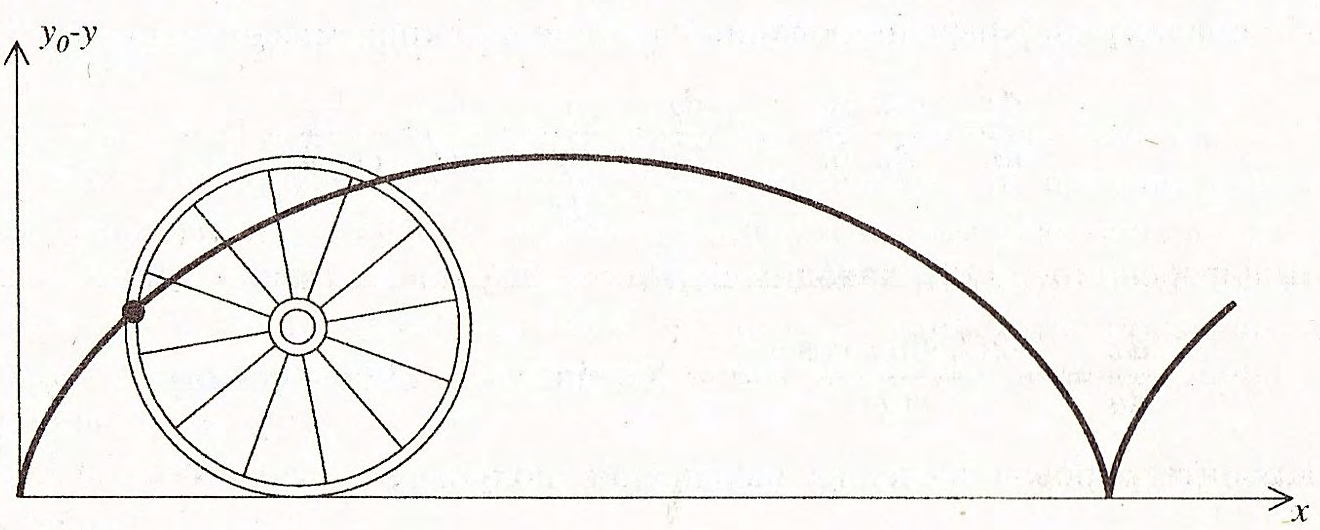
\includegraphics[width=0.8\textwidth]{../Graphics/Lectures-12-cycloid.png}
					\caption{\footnotesize Циклоида \copyvar{С. 22.}}
			\end{subfigure}
		\end{figure}
	
		Видим, что кривой наименьшего спуска является циклоида.

	\subsection{Более сложные задачи}

		Для решения некоторых задач вариационного исчисления может потребоваться большее число функций или
		независимых переменных. К примеру, задача нахождения геодезической кривой, в которой требуется найти
		$x(t), y(t), z(t)$, которые определяют кратчайший путь между двумя точками на поверхности трёхмерной
		фигуры.

		Рассмотрим подобные случаи.

		\subsubsection{Задача с несколькими функциями}

			Итак, если есть несколько функций $y$:
			$$F = F(x, y_1, y_1', y_2, y_2',\ldots)$$

			Тогда просто записывается система уравнений Эйлера:
			$$\left\{
			\begin{aligned}
				F_{y_1} - \frac{d}{dx}F_{y_1'} = 0 \\
				\dots\\
				F_{y_n} - \frac{d}{dx}F_{y_n'} = 0
			\end{aligned}
			\right.$$

		\subsubsection{Задача с производными высоких порядков}

			Рассмотрим случай, когда появляются производные более высоких порядков. 
			$$F = F(x, y, y', \ldots, y^{(k)})$$
			
			Как и раньше, введём функцию $J(\varepsilon) = I[y + \varepsilon h]$. $J'(\varepsilon)$. Её
			производная запишется следующим образом:

			$$J'(\varepsilon)\lims{\varepsilon = 0}{} = \int_{x_0}^{x_1} (F_y h(x) + F_{y'}h'(x) 
			+ F_{y''}h''(x) + \ldots + F_{y^{(k)}}h^{(k)})\,dx$$

			Первое слагаемое ранее уже интегрировали по частям: 
			$$\int_{x_0}^{x_1} F_{y'}h'(x)\,dx~=~-~\int_{x_0}^{x_1} h(x)\left(\frac{d}{dx} F_{y'}\right)\,dx$$

			Рассмотрим таким же образом следующее слагаемое:

			$$\int_{x_0}^{x_1} F_{y''}h'' \,dx = \off{h'(x)F_{y''}\lims{x_0}{x_1}} - \int_{x_0}^{x_1} h'(x)\frac{d}{dx}F_{y''} \,dx
	  		= \off{-h(x)\frac{d}{dx} F_{y''}\lims{x_0}{x_1}} + \int_{x_0}^{x_1} h(x) \frac{d^2}{dx^2}F_{y''} \,dx$$

			Как и ранее, выделенные серым слагаемые равняются нулю из-за того, что функции $h^{(k)}(x)$ равны
			нулю на краях отрезка $[x_0, x_1]$.

			Преобразовав все слагаемые таким образом, перепишем $J'(\varepsilon)$:
			$$\int_{x_0}^{x_1} h(x)
				\underbrace{\left(F_y - \frac{d}{dx}F_{y'} + \frac{d^2}{dx^2}F_{y''} - 
				\ldots + (-1)^k\frac{d^k}{dx^k}F_{y^{(k)}}\right)}_{f(x, y, \ldots, y^{(k)})} \,dx$$

			Так же как и раньше, необходимым условием будет являться выполнение уравнения $f = 0$.
	
			\begin{equation} \label{eq:EulerPoisson}
				F_y - \frac{d}{dx}F_{y'} + \frac{d^2}{dx^2}F_{y''} - 
				\ldots + (-1)^k\frac{d^k}{dx^k}F_{y^{(k)}} = 0
			\end{equation}
	
			Уравнение (\ref{eq:EulerPoisson}) называется \textbf{уравнением Эйлера-Пуассона}.

		\subsubsection{Задача с несколькими независимыми переменными}

			Осталось рассмотреть ситуацию, когда возникает несколько независимых переменных. Тогда рассмотрим
			функцию $z = z(x,y)$ и функционал:

			$$I[z] = \underset{D\hspace{10pt}}{\iint} F(x, y, z, z'_x, z'_y) \,dxdy$$
	
			Здесь мы снова введём $h \in C^{\infty}$, $\supp(h) \subset D$, где $D$ --- открытая область.
			Также введём $J(\varepsilon) = I[z + \varepsilon h]$ и снова запишем её производную:

			$$J'(\varepsilon)\lims{\varepsilon = 0}{} = 
	  		\underset{D\hspace{10pt}}{\iint} (F_zh + \underline{F_{z'_x}h'_x} + \underline{F_{z'_y}h'_y}) \,dxdy$$

			Чтобы получить уравнение на экстремали, нужно получить $h(x)$ вместо её производных в
			подчёркнутых слагаемых.
	
			\begin{align*}
				\frac{d}{dx}(h F_{z'_x}) = \underline{h'_xF_{z'_x}} + h\frac{d}{dx}F_{z'_x} \\
				\frac{d}{dy}(h F_{z'_y}) = \underline{h'_yF_{z'_y}} + h\frac{d}{dy}F_{z'_y}
			\end{align*}

			Перепишем $J(\varepsilon)$, выразив подчёркнутые слагаемые:
	
			$$
				J'(\varepsilon)\lims{\varepsilon = 0}{} = 
				\underset{D\hspace{10pt}}{\iint} \left( h\cdot\left(F_z - \frac{d}{dy}F_{z'_y} - \frac{d}{dx}F_{z'_x}\right) \right) \,dxdy
				+ \underset{D\hspace{10pt}}{\iint} \left(\frac{d}{dx}(hF_{z'_x}) + \frac{d}{dy}(hF_{z'_y}) \right) \,dxdy
			$$

			Второй интеграл может быть преобразован по теореме Стокса из векторного анализа. В двумерном случае (часто называемом формулой Грина):

			$\iint_{D} (P\,dx + Q\,dy) = \oint_{\partial D} (Q_x - P_y) dx dy$.

			Отсюда получаем:

			$$
				J'(\varepsilon)\lims{\varepsilon = 0}{} = 
				\underset{D\hspace{10pt}}{\iint} \left( h\cdot\left(F_z - \frac{d}{dy}F_{z'_y} - \frac{d}{dx}F_{z'_x}\right) \right) \,dxdy
				+ \underbracket{\underset{\partial D}{\oint} \left(hF_{z'_x}\,dy + hF_{z'_y}\,dx \right)}_{=0}
			$$

			Второй интеграл равняется нулю, так как функция $h(x, y)\lims{\partial D}{} \equiv 0$ потому что $\supp(h) \subset D$.

			Полученное уравнение
			$$F_z - \frac{d}{dy}F_{z'_y} - \frac{d}{dx}F_{z'_x} = 0$$
			называется \textbf{уравнением Эйлера-Остроградского}.

			\example{Интеграл Дирихле}. Рассмотрим функционал вида 
	
				$$I[z] = \iint\limits_D (z_x'^2 + z_y'^2)^2 \,dxdy$$
	
				Рассматриваемый интеграл называется интегралом Дирихле. Получим выражение для экстремалей
				функционала $I[z]$.
	
				$$\off{F_z} - \frac{d}{dy} F_{z'_y} - \frac{d}{dx} F_{z'_x} = 0$$
				$$-\frac{d}{dy} 2z'_y - \frac{d}{dx} 2z'_x = 0$$
				$$z''_{yy} + z''_{xx} = 0$$
	
				Таким образом, экстремалями этого функционала являются гармонические функции.

		\subsubsection{Задача с незакреплёнными концом. Условие трансверсальности}

			$$I[y] = \int_{x_0}^{x_1} F(x, y, y')dx \qquad y(x_0) = y_0$$
	
			\begin{figure}
				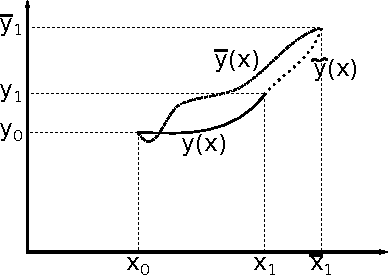
\includegraphics[width=0.8\textwidth]{./../Graphics/Lectures-12-unknowntask.pdf}
			\end{figure}
	
			Продолжим функцию $y(x)$ так, чтобы её продолжение $\tilde{y}(x) \in C^1$.
	
			Введём $\rho(y, \tilde{y}) = \norm{y - \tilde{y}} + \sqrt{(x_1 - \bar{x_1})^2 + (y_1 - \bar{y_1})^2}$. Назовём $\rho$ расстоянием между двумя этими функциями.

			Для дальнейших вычислений введём следующие обозначения:
	
			$$
				\left\{
				\begin{aligned}
					h(x) = \overline{y} - y \\
					\delta x = \overline{x_1} - x_1
					\delta y = \overline{y}(x_1) - y(x_1)
				\end{aligned}
				\right.
			$$

			$$I[\overline{y}] - I[y] = 
	  			\underbracket{\int_{x_0}^{x_1} (F(x, y + h, y' + h') - F(x, y, y')) \,dx}_{I_1} +
	  			\underbracket{\int_{\overline{x}_0}^{\overline{x}_1} F(x, \overline{y}, \overline{y}') \,dx}_{I_2}$$
	  
			В подынтегральном выражении для $I_2$ стоит непрерывная функция. Значит, можем воспользоваться
			теоремой о среднем.
	
			\opt{
				\begin{theorem*}
					Пусть функция f(x) непрерывна на $[x_1, \overline{x}_1]$, тогда 
					$\exists x_C\in[x_1,\overline{x}_1]\;\;
					\int\limits_{x_1}^{\overline{x}_1}f(x)dx = f(x_C)(\overline{x}_1 - x_1)$.
				\end{theorem*}
			}
	
			Положим некоторое значение $x_C \in [x_0, x_1]$. Тогда 
			$$I_2 = \delta x_1 F(x, \overline{y}, \overline{y}')\lims{x = x_C}{} 
			= \delta x_1 F\big(x_1, \overline{y}(x_1), \overline{y}'(x_1)\big) + o(\delta x_1)$$
	
			Приращение интеграла $I_1$ можно записать по формуле Тейлора:
			$$f(x + h) = f(x) + df(x) \angular{h} + o(\mod{h})$$
			Таким образом, 
			$$I_1 = \int_{x_0}{x_1} (F_yh - F_{y'}h') \,dx + o\big(\rho(y, \overline{y})\big)$$
	
			$o(\ldots)$ ушло из подынтегрального выражения, так как интеграл берётся по конечному промежутку,
			а умножение $o(\ldots)$ на константу ничего не меняет. Итак, интегрируем второго слагаемое по
			частям:
	
			$$I_1 = \int_{x_0}{x_1} h\cdot(F_y - \frac{d}{dx}F_{y'}) \,dx + hF_{y'}\lims{x_0}{x_1} + o(\ldots) = \int_{x_0}^{x_1} h\cdot(F_y - \frac{d}{dx}F_{y'}) \,dx + h(x_1) F_{y'}\lims{x = x_1}{}$$

			\lecture{13}

			Отсюда получаем:

			$$\Delta I = \int_{x_0}^{x_1} (F_y - \frac{d}{dx} F_{y'})h(x)\,dx + h(x_1)F_{y'}\lims{x=x_1}{} + 
	  		F\lims{x=x_1}{}\cdot \delta x_1 + o(\rho(y,\tilde{y}))$$

			Преобразуем $h(x_1)$. Как было записано ранее, $h(x_1) = \bar{y}(x_1) - y(x_1)$:

			$$\bar{y}(\bar{x}_1) - \bar{y}(x_1) = y'(x_1 + \theta \delta x_1)\cdot \delta x_1 
			= y'(x_1) \delta x_1 + o(\rho(y, \bar{y}))$$

			Тогда сможем выразить $\bar{y}$ через $y$:
			$$h(x_1) = \bar{y}(x_1) - y(x_1) = \underbracket{\bar{y}(\bar{x}_1) - y(x_1)}_{\delta y_1}
	  		- y'(x_1)\delta x_1 + o(\rho(y, \bar{y}))$$

			\begin{align*}
				\Delta I = \int_{x_0}^{x_1} \left(F_y - \frac{d}{dx}F_{y'}\right)h(x)\,dx
				+ \delta x_1\cdot(F - y'F_{y'}) \lims{x=x_1}{}
				+ \delta y_1 \cdot F_{y'}\lims{x=x_1}{}
			\end{align*}

			В вариационном исчислении величина $\Delta I$ зачастую называется вариацией функционала (по
			аналогии с дифференциалом функции). Необходимым условием экстремума будет $\Delta I = 0$. Таким
			образом, приходим к следующим уравнениям:

			\begin{equation}
				\label{eq:preTraversal}
				\begin{cases}
				&F_y - \frac{d}{dx} F_{y'} = 0 \\
				&(F - y'F_{y'})\lims{x = x_1}{} \delta x_1 + F_{y'} \lims{x=x_1}{}\delta y_1 = 0
				\end{cases} 
			\end{equation}

			\off{(Без доказательства)} Если решать задачу где и левый конец функции тоже не закреплён, то
			$\Delta I$ запишется как:
			\begin{align*}
				\Delta I = \int_{x_0}^{x_1} (F_y - \frac{d}{dx}F_{y'})h(x)\,dx~+~ 
				\delta x\cdot(F - y'F_{y'})\lims{x = x_0}{x = x_1}~+~ \\
				~+~\delta y_1 \cdot F_{y'} \lims{x=x_1}{}-~\delta y_0 \cdot F_{y'} \lims{x=x_0}{}
			\end{align*}

			\opt{\off{Популярными граничными условиями являются $F_{y'}\lims{x=x_0}{}=F_{y'}\lims{x=x_1}{}=0$}}

			\todo{Картинка}
			Если задать, что правый конец экстремали лежит на некоторой функции $\psi(x)$:
			$$\delta y_1 = \psi'(x_1) \delta x_1 + o(\delta x_1)$$

			Тогда условие (\ref{eq:preTraversal}) перепишется как:
			$$
				\begin{cases}
					&F_y - \frac{d}{dx} F_{y'} = 0 \\
					&\delta x_1 \cdot (F - y'F_{y'} + \psi' F_{y'})\lims{x=x_1}{} + o(\delta x_1) = 0
				\end{cases} 
			$$

			Уравнение
			\begin{equation}
				\label{eq:traversal}
				(F - y' F_{y'} + \psi' F_{y'})\lims{x=x_1}{} = 0
			\end{equation}
			называется \textbf{условием трансверсальности}.

			Рассмотрим частный случай, когда функция $F$ имеет вид $F(x, y, y') = f(x,y) \sqrt{1+y'^2}$.
			Подставляя $F$ в \ref{eq:traversal}, получаем:

			$$
				\left( f \sqrt{1+y'^2} - y' f \frac{y'}{\sqrt{1+y'^2}} + \psi' f \frac{y'}{\sqrt{1+y'^2}} \right) \lims{x=x_1}{}
			$$

			После простых преобразований получаем упрощённое условие трансверсальности:

			$$\left( \psi' y' \right) \lims{x=x_1}{} = -1$$

			Производные от функций можно трактовать как коэффициент наклона касательной в точке $x=x_1$, а равенство их произведения $-1$ означает перпендикулярность этих касательных. Таким образом, в случае, если $F(x, y, y') = f(x,y) \sqrt{1+y'^2}$, то оптимальным путём будет тот, который придёт в точку $x=x_1$ перпендикулярно функции $\psi(x)$.

	\subsection{Решение изопериметрической задачи}

		\todo{перепроверить, местами чушь написана}

		Пусть даны функции 
		$$x(t),\qquad y(t)$$
		с заданными граничными условиями:
		$$x(t_0) = x(t_1) = x_0 \qquad y(t_0) = y(t_1) = y_0$$

		Задача --- максимизировать площадь $S[x,y] = \int_{t_0}^{t_1}x(t)y'(t) dt$ при условии, что периметр
		$l[x,y] = \int_{t_0}^{t_1} \sqrt{\dot{x}^2(t) + \dot{y}^2(t)}\,dt$ фиксирован.

		В более общей формулировке задача звучит так: найти минимум функционала
		$I[y] = \int_{x_0}^{x_1} F(x,y,y')\,dx$, если несколько функционалов того же вида постоянны
		$J_k[y] = \int_{x_0}^{x_1} G_k(x,y,y')\,dx = C_k$. (Если считать $G_k$ дельта-функцией, то граничные
		условия тоже можно записать в таком виде.)

		Для нахождения экстремума в многомерном случае в курсе математического анализа рассматривается
		равенство нулю скалярного произведения градиента на касательную к многообразию. Нужно, чтобы
		производная вдоль любого вектора, касательного к поверхности,

		\begin{equation}g_i(x) = C_i, \qquad g_1\ldots g_m \label{eq:Surface}\end{equation}

		равнялась нулю. В выбранной точке $x$ касательное пространство является ортогональным дополнением
		к $m$ градиентам из (\ref{eq:Surface}). Следовательно, обязательным образом
		
		$$\nabla f = \sum_i \lambda_i \nabla g_i \quad \Rightarrow \quad f = \sum_i \lambda_i g_i$$

		С этими утверждениями из математического анализа вы уже знакомы. Теперь рассмотрим, как они
		применяются в нашей задаче. Нужно, чтобы вариация функционалов $J_k$ равнялась нулю:
		$\delta J_k = 0$.

		На каждое $G_k$ получается уравнение
		$$\int_{x_0}^{x_1} \left(\underline{G_{k_y} - \frac{d}{dx}G_{k_{y'}}}\right) h(x)\,dx = 0$$	
		где подчёркнутое выражение играет роль градиента. Таким образом,
		$$\delta I = \int_{x_0}^{x_1} \left(F - \frac{d}{dx}F_{y'}\right)h(x) \,dx 
	  	= \int_{x_0}^{x_1} \left(\sum_i \left(\lambda_i G_{i_y} - \frac{d}{dx}G_{i_{y'}} \right)\right)h(x) 			\,dx$$
	  
		Таким образом, должно выполняться условие
		\todo{Наверное, здесь должно быть $h(x)$}
		$$\int_{x_0}^{x_1} \left(F - \sum_i \lambda_i G_i\right) \,dx = 0$$

		Ничего не мешает нам считать, что $F(\ldots) = G_0$, тогда $\lambda_0 = 1$. Так как 
		$F$ и $G_i$ --- функции одинакового вида, можно внести $F$ в граничные условия и решать
		задачу для какого-нибудь $G_i$. Эти высказывания формируют \textbf{принцип взаимности}.

		\off{Таким образом, изопериметрическая задача равносильна нахождению минимального периметра при 
		фиксированной площади.}

	\subsection{Нахождение геодезических кривых}

		\begin{defi}
			\textbf{Геодезическая кривая} --- кратчайшая кривая, соединяющая две точки на поверхности.
		\end{defi}

		Не будем приводить здесь доказательства рассматриваемого метода, просто представим его <<рецепт>>.

		В качестве примера рассмотрим задачу о нахождении геодезических кривых на поверхности сферы.
		Рассматривается функционал следующего вида:
		$$I[x] = \int_{t_0}^{t_1} F(t,x,\dot{x})\,dt \qquad x \in \mathbb{R}^n$$

		То есть существует $n$ функций, описывающих путь по искомой кривой. В исходной задаче такой
		функционал равен $F(t,x,\dot{x}) = \sqrt{\dot{x}^2 + \dot{y}^2 + \dot{z}^2}$, то есть длине
		пути.

		Потребуется ввести граничные условия, ограничивающие область поиска:
		\begin{equation} \label{eq:GeodSurface}
			g_i(t, x, \dot{x}) = 0 \qquad i = 1,\ldots k \qquad
			\begin{aligned}
				x(t_0) = x_0 \\
				x(t_1) = x_1
			\end{aligned}
		\end{equation}

		Рассмотрим ещё один функционал:

		\todo{Здесь, видимо, тоже должно быть $h(x)$}
		$$J[x] = \int_{t_0}^{t_1} \left(F(t,x,\dot{x}) + \sum_{i=1}^k \lambda_i(t) g_i(t)\right)\,dt$$

		Сделаем важное предположение: для $F(\ldots)$, экстремали функционала $I[x]$, обязятельно найдётся
		$k$ функций $\lambda_i(t)$, таких, что решение будет представляться экстремалями функционала $J[x]$.
		При этом, $\lambda_i(t)$ находятся из уравнения Эйлера и граничных условий (\ref{eq:GeodSurface}).

	\subsection{Уравнение колебаний струны}

		\todo{Добавить из семинаров поиск уравнения колебания струны!}

\end{document}

\end{document}
